\documentclass[a4paper,11pt]{article}
	
\usepackage[english]{babel}
\usepackage{soul}
\usepackage{mathtools}
\usepackage{amssymb,amsmath,amsfonts}
\usepackage[utf8]{inputenc}
\usepackage{graphicx}
\usepackage{geometry}
\usepackage{float}
\usepackage{csquotes}
\PassOptionsToPackage{hyphens}{url}\usepackage{hyperref}
\usepackage{fancyhdr}
\usepackage{gensymb}
\usepackage{hhline}
\usepackage{siunitx}
\usepackage[table,dvipsnames]{xcolor}
\usepackage[export]{adjustbox}
\usepackage[nottoc,numbib]{tocbibind}
\usepackage[super,comma]{natbib}
\usepackage{titling}
\usepackage[italian]{datetime}
%\usepackage{subfigure}
\usepackage{subcaption}
\usepackage{cancel}
\usepackage{comment}
\definecolor{blunipi}{RGB}{0,111,141}
     \usepackage{verbatim}
     \usepackage{pdflscape}
     \usepackage{booktabs}
\usepackage{multirow}
\usepackage{bigstrut}
\usepackage{wrapfig}


\newcommand\eqeg{\stackrel{\mathclap{\normalfont\mbox{e.g.}}}{=}}
\newcommand{\charactercount}[1]{
\immediate\write18{
expr `texcount -1 -sum -merge #1.tex` + `texcount -1 -sum -merge -char #1.tex` - 1 
> chars.txt
}\input{chars.txt}}




%\captionsetup[figure]{labelformat=empty}

%\renewcommand{\today}{\thisdayofweekname\ \theday\ \monthname\ \the\year}

\geometry{a4paper, left=20mm, right=20mm, top=25mm, bottom=25mm}

\title{Telco Costumer Churn analysis} 
\author{Intorduction to Machine Learning}
\date{\today}

\pagestyle{empty}
%\lfoot{Tesi di Laurea in Fisica}
%\rfoot{Giulio Cordova} 

\begin{document}
    \newgeometry{left=20mm, right=15mm, top=12mm, bottom=10mm}
    %\begin{titlepage}
        \thispagestyle{empty}
        \begin{figure}
            
\includegraphics[width=60mm,right]{./1 logo.png}
        \end{figure}
        \vspace*{-38mm}\hspace{-6mm}\textbf{\textcolor{blunipi}{\large{Scuola Normale Superiore}}}\\\\
        \hspace{-2mm}\textcolor{blunipi}{\large{Classe di Scienze}}
        
        \vspace{15mm}
        \begin{center}
            \textcolor{blunipi}{\huge{\textbf{\thetitle}}}\\\vspace*{7mm}
        \textcolor{blunipi}{\theauthor}\\\vspace*{10mm}
            \textcolor{blunipi}{\thedate}\\\vspace*{10mm}
            
            %Forse i margini dovrebbero andare un po' più stretti
            \begin{tabular}{rl}
                \textbf{Author:} 
                & Giulio Cordova \\ 
                & \\
                & \texttt{giulio.cordova@sns.it}\\\\
                
                %\textbf{Relatore:} 
                %& Giovanni Punzi \\
                %& \texttt{paulo.azzurri@cern.ch}\\\\
                
            \end{tabular}
            \vspace*{5mm}
\end{center}
\tableofcontents
    \restoregeometry
    \setcounter{page}{1}
\pagestyle{plain}
\section{Data Understanding \& Preparation}
The \textit{Telco Customer Churn} dataset includes 7043 customer records and 21 variables, covering demographics, service subscriptions, contract details, and churn status (i.e., whether the customer left in the last month). The features can be grouped into four categories:

\begin{itemize}
\item \textbf{Demographics:} \texttt{gender}, \texttt{SeniorCitizen}, \texttt{Partner}, and \texttt{Dependents}. Most are categorical (\texttt{Yes}/\texttt{No}); \texttt{SeniorCitizen} is binary (0/1).
\sloppy
\item \textbf{Contract Details:} \texttt{tenure} (subscription duration), \texttt{Contract}, \texttt{PaperlessBilling}, and \texttt{PaymentMethod}. \texttt{Contract} and \texttt{PaymentMethod} are multi-category variables, while \texttt{PaperlessBilling} is boolean.

\item \textbf{Subscribed Services:} Indicators for phone, internet, and additional services (e.g., \texttt{OnlineSecurity}, \texttt{StreamingTV}). Most of these are categorical but can be interpreted as boolean. Several variables also include the redundant category \texttt{No internet service}, repeated across all add-on features.

\item \textbf{Target:} \texttt{Churn}, a binary categorical variable indicating customer loss.
\end{itemize}

After loading the CSV file, columns and data types were reviewed. The \texttt{TotalCharges} column, although numerical by nature, was initially read as an object due to malformed entries. After coercing it to a numeric type, 11 missing values were identified and dropped, given their limited number. Additionally, 22 duplicate rows were found and removed.

Many categorical features in the dataset are binary in nature and were therefore converted to boolean variables. A dedicated routine was implemented to automate this process and ensure consistency. In particular, the variables \texttt{PhoneService}, \texttt{MultipleLines}, \texttt{OnlineSecurity}, \texttt{OnlineBackup}, \texttt{TechSupport}, \texttt{StreamingTV}, \texttt{StreamingMovies}, and \texttt{DeviceProtection} were converted into boolean form. For these, the special values \texttt{No phone service} or \texttt{No internet service} were interpreted as \texttt{False}, since the presence of phone or internet service is already captured by other variables. The variable \texttt{gender} was transformed into a new binary feature named \texttt{IsMale}, equal to \texttt{True} if the customer is male, and \texttt{False} otherwise. Multi-category features like \texttt{Contract}, \texttt{InternetService}, and \texttt{PaymentMethod} were one-hot encoded.

Numerical variables were scaled to [0, 1] using MinMaxScaler. This normalization was important for correlation analysis, dimensionality reduction, and clustering.

Correlation analysis was conducted using Pearson correlation. The results confirmed intuitive relationships: \texttt{TotalCharges} is positively correlated with both \texttt{tenure} and \texttt{MonthlyCharges}; customers with additional services such as \texttt{StreamingTV}, \texttt{StreamingMovies}, or \texttt{Fiber optic} tend to pay higher monthly charges. Regarding the target variable \texttt{Churn}, it showed positive correlation with \texttt{Month-to-month} contracts, \texttt{Fiber optic} internet, and \texttt{Electronic check} payments, while it was negatively correlated with \texttt{tenure} and \texttt{Two year} contracts.

As a final step, Principal Component Analysis (PCA) was applied to the standardized numerical dataset to investigate its internal structure and to reduce its dimensionality. Importantly, the target variable \texttt{Churn} was excluded from this analysis, as this dataset will be used for clustering analysis and a goal of clustering is to uncover natural groupings in the data independent of the known labels. The PCA revealed that the first 21 princiapl components (PCs) accounted for more than 99\% of the total variance, indicating that the remaining components contributed negligibly to the overall information content. This strong compression is largely due to redundancy among features—\texttt{TotalCharges}, for example, is a linear combination of \texttt{tenure} and \texttt{MonthlyCharges}. Based on this insight, the dataset was projected onto the first 21 PCs and this reduced representation was saved for use in subsequent clustering experiments.

% Example for including a figure:
% \begin{figure}[h]
% \centering
% \includegraphics[width=0.7\linewidth]{pca_plot.png}
% \caption{Projection of the dataset onto the first two PCA components.}
% \end{figure}
\section{Clustering}
The dataset used for clustering is the PCA-transformed version described earlier, which retains 21 PCs to reduce dimensionality and eliminate redundancy among the original features. In this representation, all variables are continuous numerical values, and no longer boolean or categorical.

\subsection{K-Means}
To determine the optimal number of clusters $K$, the K-Means algorithm was run for values of $K$ ranging from 2 to 50. The Elbow Method was then applied, revealing a clear inflection point at $K = 6$, which was chosen as the final number of clusters.

Clusters were visualized through pairwise projections of the first three principal components, with a 3D scatter plot of the first three PCs also available in the notebook.

\begin{figure}[h]
\centering
\begin{subfigure}{0.32\linewidth}
    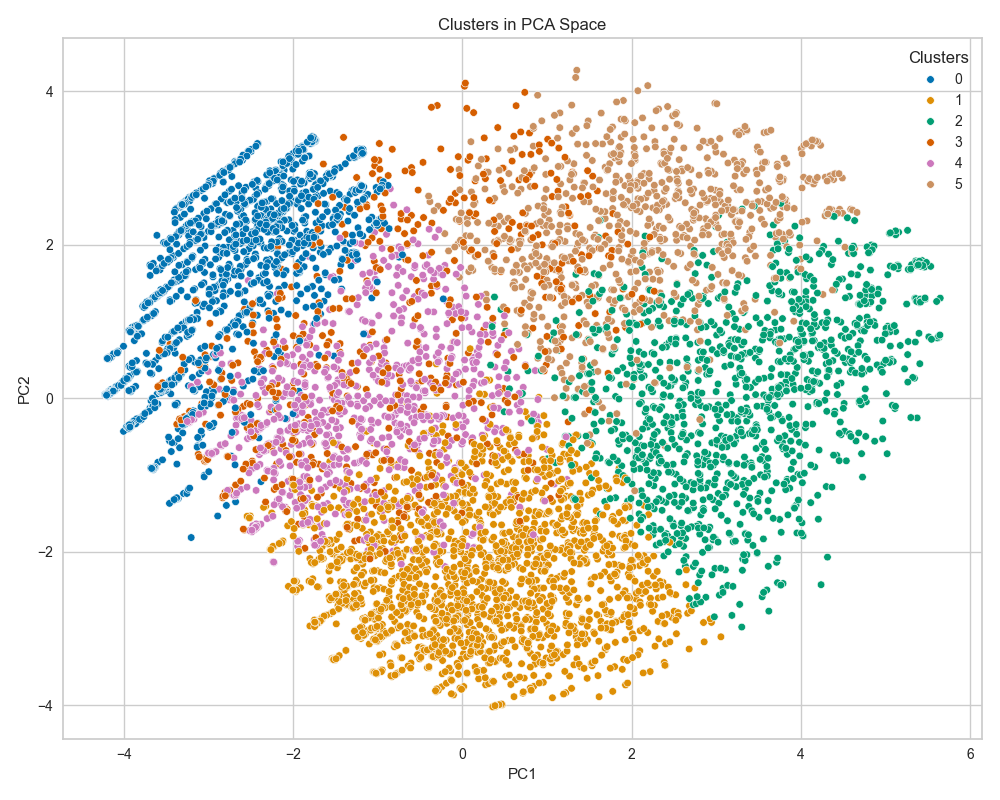
\includegraphics[width=\textwidth]{figures/clustering/6-means_pca_12.png}
    \caption{Projection in PC1-PC2 Plane}
    \label{fig:cluster_12}
\end{subfigure}
\hfill
\begin{subfigure}{0.32\linewidth}
    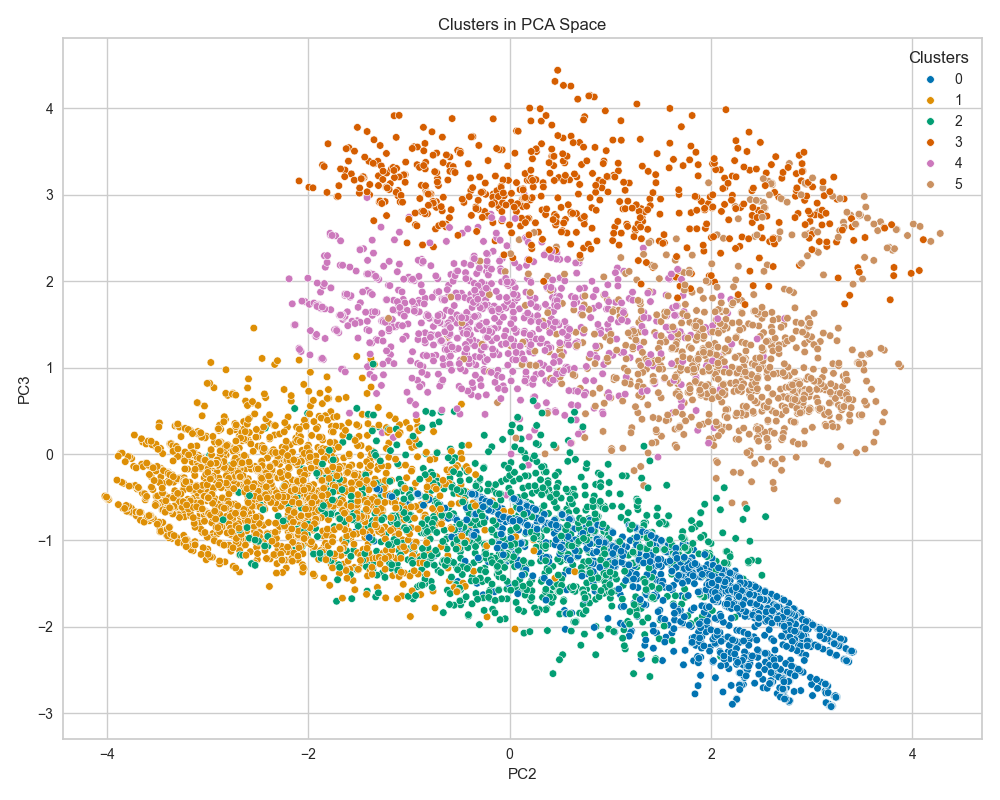
\includegraphics[width=\textwidth]{figures/clustering/6-means_pca_23.png}
    \caption{Projection in PC2-PC3 Plane}
    \label{fig:cluster_23}
\end{subfigure}
\hfill
\begin{subfigure}{0.32\linewidth}
    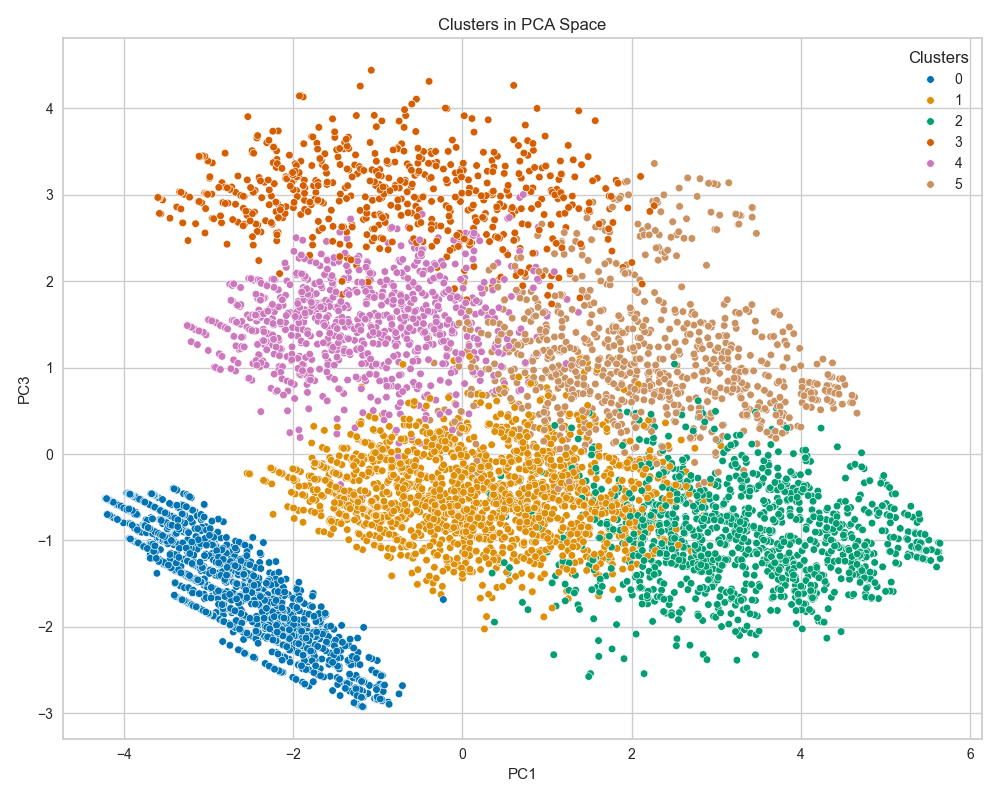
\includegraphics[width=\textwidth]{figures/clustering/6-means_pca_13.png}
    \caption{Projection in PC1-PC3 Plane}
    \label{fig:cluster_13}
\end{subfigure}
\caption{Color-coded clusters found with 6-Means clustering in the PCA space}
\label{fig:clusters_pca}
\end{figure}


For each cluster, I analysed the distribution of the original features and produced summary bar plots like the one shown in Figure~\ref{fig:cluster_5}. In these plots, features are ordered by the variance of their mean values across all clusters, helping to highlight which variables are most informative in differentiating between groups.
\begin{figure}[h]
\centering
\begin{subfigure}{\linewidth}
    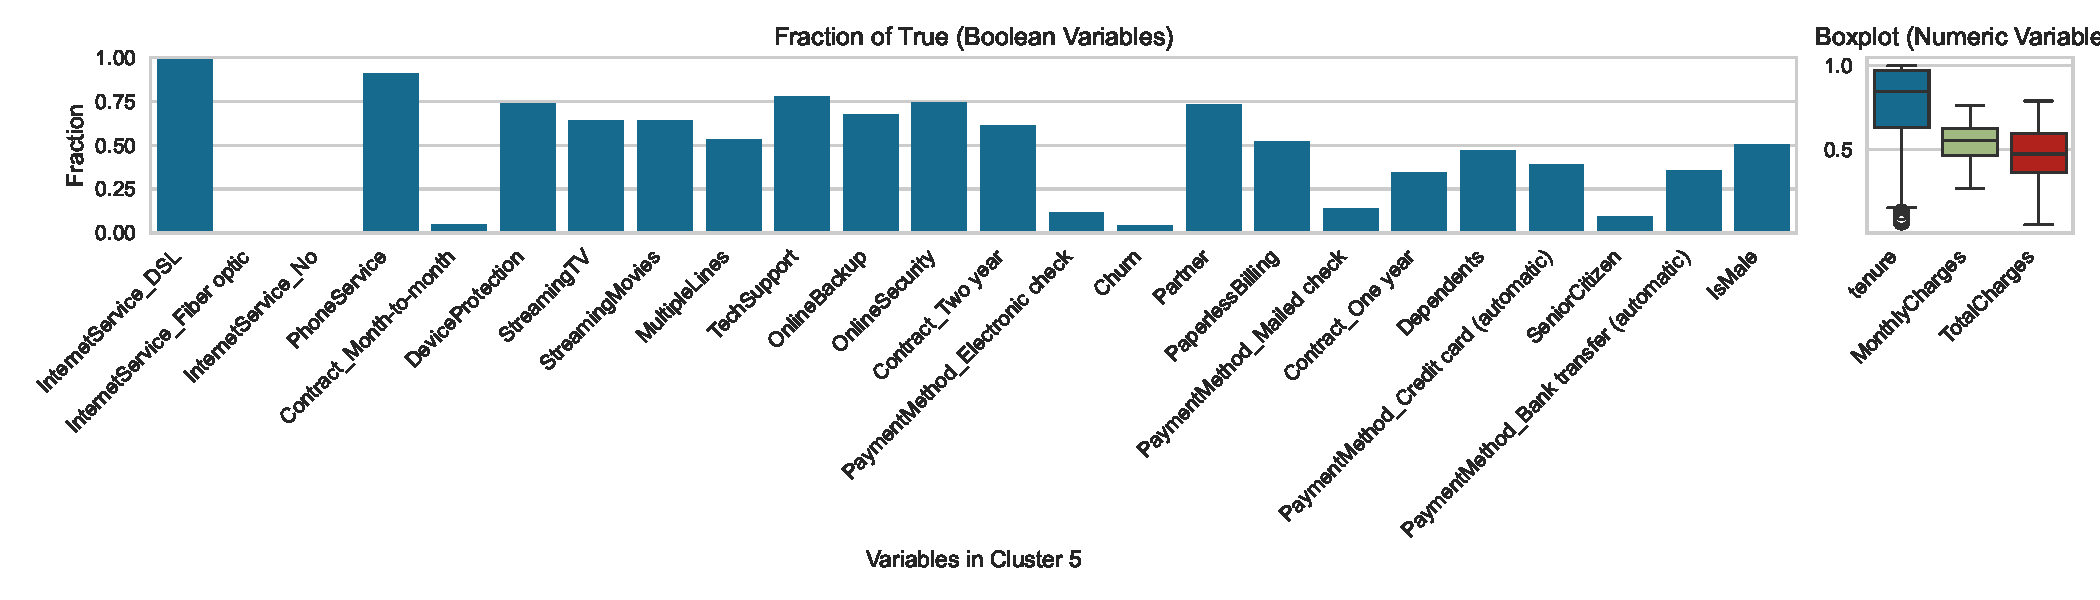
\includegraphics[width=\linewidth]{figures/clustering/cluster_5_clusters.pdf}
\caption{Cluster 5}
\label{fig:cluster_5}
\end{subfigure}
\begin{subfigure}{\linewidth}
    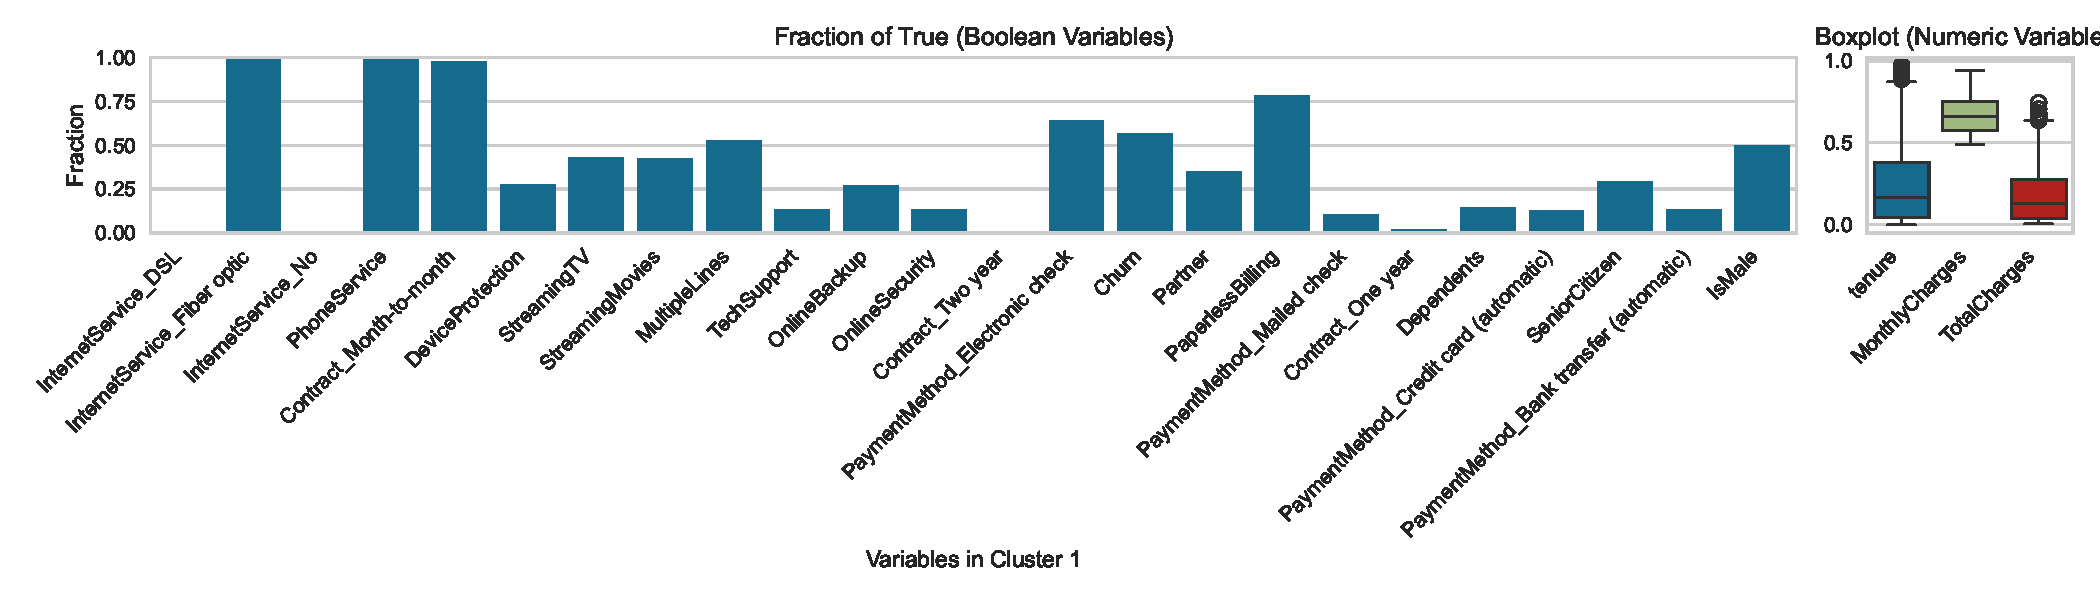
\includegraphics[width=\linewidth]{figures/clustering/cluster_1_clusters.pdf}
\caption{Cluster 1}
\label{fig:cluster_1}
\end{subfigure}
\caption{Distribution of features in the clusters. For the boolean features only the percentage is reported in the form of a bar plot, while the distribution of the normalized numerical features is represented with boxplots}
\end{figure}
The goal of this analysis was to identify natural profiles of customers represented by each cluster. For example:
\begin{itemize}
\item \textbf{Cluster 5} contains users with long tenure, partners and dependents, and a wide range of internet services such as streaming or tech support. The churn rate in this group is low, suggesting that it may represent satisfied families with well-tailored contracts.
\item \textbf{Cluster 1} includes users with high monthly charges and short tenure. These users often have fiber optic internet and additional services, but also a higher proportion of senior citizens. This may suggest customers who are paying for more than they need, leading to a higher churn rate.
\end{itemize}

Similar reasoning could be applied to other clusters, each potentially representing a different customer archetype.

\subsection{DBSCAN}
To determine an appropriate value for the $\epsilon$ parameter in DBSCAN, I performed a K-nearest-neighbor (KNN) analysis with $K=5$. The resulting distance plot (in appendix) suggested the presence of multiple possible density thresholds, indicating that DBSCAN might struggle with this dataset due to the presence of clusters with varying densities.

Nonetheless, I attempted clustering with several $\epsilon$ values. The best configuration identified approximately 10 clusters, although only 45\% of the data points were classified as belonging to a cluster—the rest were labeled as outliers. Although I produced similar summary plots as for K-Means to analyze the resulting groups, I decided not to include those results in this report due to the limited interpretability and the high number of outliers.

\subsection{Hierarchical Clustering}
Using the Euclidean distance metric, I evaluated several linkage methods: single, complete, average, and Ward’s method. Among these, average and complete linkage performed best, as assessed by both the Silhouette Score and the Calinski-Harabasz Index.
\subsection{Comparison}
A comparison between the clustering algorithms was carried out using the Silhouette score and the Calinski-Harabasz (CH) score. The results are reported in Table~\ref{tab:clustering_metrics_transposed}. The highest Silhouette score is achieved by DBSCAN; however, as discussed earlier, DBSCAN tends to classify a large portion of the data points as outliers, which limits its effectiveness in this case. On the other hand, the CH score indicates that K-Means performs best, followed closely by hierarchical clustering using the \texttt{complete} and \texttt{average} linkage methods.

\begin{table}[h]
\centering
\resizebox{\textwidth}{!}{%
\begin{tabular}{lcccccc}
\toprule
\textbf{Metric} & \texttt{K-Means} & \texttt{hier\_complete} & \texttt{hier\_average} & \texttt{hier\_ward} & \texttt{DBSCAN} & \texttt{hier\_single} \\
\midrule
Silhouette & 0.134388 & 0.140719 & 0.154223 & 0.127726 & \textbf{0.180492} & -0.071615 \\
Calinski-Harabasz & \textbf{838.415150} & 802.136304 & 781.315251 & 733.134051 & 386.018306 & 1.240939 \\
\bottomrule
\end{tabular}%
}
\caption{Comparison of clustering algorithms using Silhouette and Calinski-Harabasz scores.}
\label{tab:clustering_metrics_transposed}
\end{table}
\section{Classification}
The goal of this task is to train and evaluate different classifiers to predict the target variable \textit{Churn}. The dataset was split into training and test sets, with the test set comprising 30\% of the original data. The methods explored include: Decision Tree, Random Forest, k-Nearest Neighbours (kNN), Linear Regression, and Logistic Regression.

\subsection{Decision Tree (DT)}
For the Decision Tree, I used the rescaled one-hot-encoded dataset, since the algorithm does not require numerical features per se. A naive implementation using the default parameters (Gini impurity, no limit on tree depth, etc.) leads to a highly complex tree, which overfits the training data and generalizes poorly to the test set.

To mitigate overfitting, I applied \textit{Cost Complexity Pruning} (CCP), governed by the parameter $\alpha$, which penalizes overly complex trees. This approach reduces the need to manually tune other hyperparameters such as \textit{max depth} or \textit{min samples leaf}.

The optimal value of $\alpha$ was determined by computing the accuracy on both training and test sets for different values of $\alpha$. To increase statistical robustness, the evaluation was repeated using 10-fold cross-validation. The final pruned tree was trained using the $\alpha$ that maximized the test accuracy. The process was repeated for both impurity measures: Gini and Entropy.

\subsection{Random Forest}
Using the same dataset as for the Decision Tree, I performed a grid search to tune the hyperparameters of the Random Forest classifier. The results are discussed in the following comparison subsection.

\subsection{k-Nearest Neighbours (kNN)}
To determine the optimal value of $k$, the algorithm was evaluated over a range of $k$ values, selecting the one that maximized the accuracy on the validation set. Results are included in the comparative analysis below.

\subsection{Linear and Logistic Regression}
\begin{wrapfigure}{r}{0.5\textwidth}
\begin{center}    
%\centering
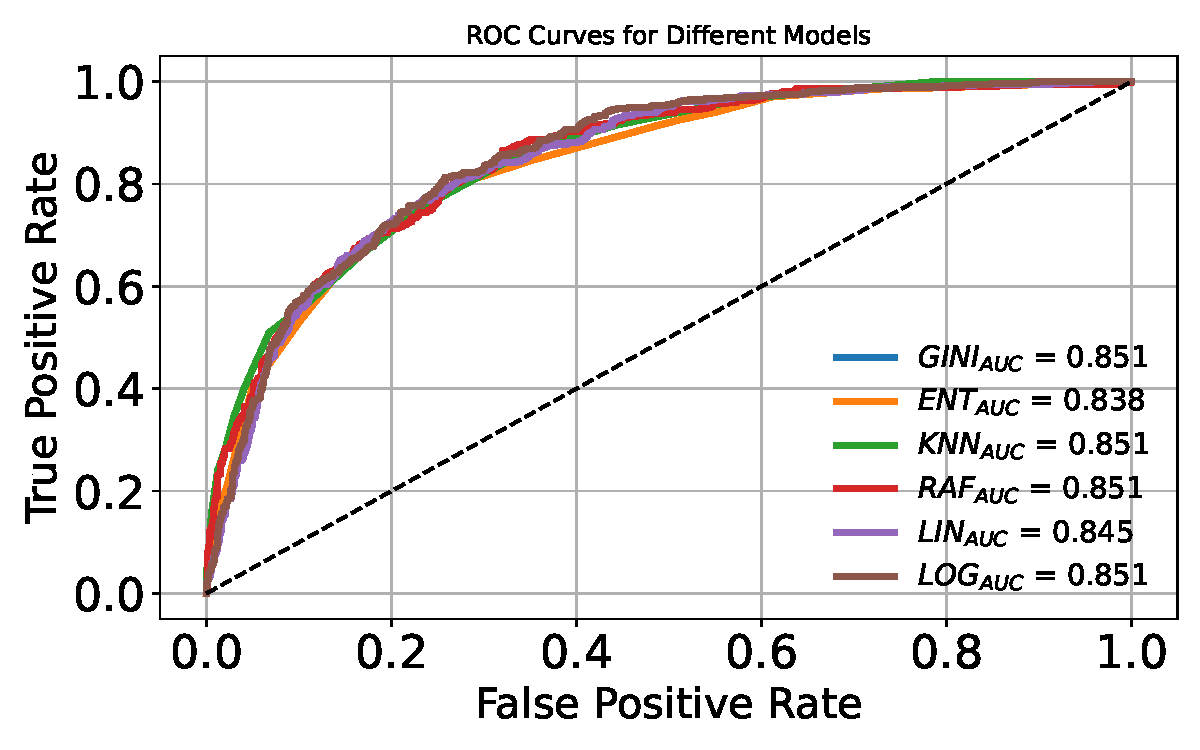
\includegraphics[width=\linewidth]{figures/classification/roc_curves.pdf}
    \end{center}
\caption{ROC curves of all tested classifiers.}
\label{fig:roc}
\end{wrapfigure}
Although Linear Regression is not ideally suited for binary classification, I experimented with it by encoding the target variable numerically (1 for churn, 0 otherwise). The model was implemented using PyTorch on a rescaled dataset (values between 0 and 1). The loss function used was the Mean Squared Error (MSE), equivalent to minimizing the $\chi^2$. The model converged after a few epochs. Results are reported in the next subsection.

Logistic Regression was also tested using the Binary Cross Entropy loss. No hyperparameter tuning was performed. Performance metrics are discussed in the next section.

\subsection{Comparison Between Classifiers}

To compare the classifiers, I used the Receiver Operating Characteristic (ROC) curve and the Area Under the Curve (AUC). Figure \ref{fig:roc} shows the ROC curves of all tested classifiers. The results indicate that all classifiers perform similarly, except for Linear Regression and the Decision Tree trained with Entropy, which performed worse.

The highest-performing classifiers reached an AUC of approximately 0.85, which is satisfactory but not optimal.
\begin{comment}
\begin{table}
\centering
\adjustbox{max width=\textwidth}{%
\begin{tabular}{|r||c|c||c|c||c|c||c|c|}
\hline
& Predicted 1 & Predicted 0 & Predicted 1 & Predicted 0 & Predicted 1 & Predicted 0 & Predicted 1 & Predicted 0 \\\hline\hline
True 1 & \cellcolor{YellowGreen}273 & 186 & \cellcolor{YellowGreen}225 & 108 & \cellcolor{YellowGreen}176 & 54 & \cellcolor{YellowGreen}311 & 143 \\\cline{1-9}
True 0 & 165 & \cellcolor{Goldenrod}1129 & 213 & \cellcolor{Goldenrod}1207 & 262 & \cellcolor{Goldenrod}1261 & 246 & \cellcolor{Goldenrod}1403 \\\hline\hline
& \multicolumn{2}{|c||}{Decision Tree} & \multicolumn{2}{|c||}{Random Forest} &
\multicolumn{2}{|c||}{kNN} & \multicolumn{2}{|c|}{Logistic Regression} \\
\hline
\end{tabular}
}
\caption{Confusion matrices for classifying the target variable with different algorithms. Green indicates True Positives, yellow indicates True Negatives.}
\label{tab:conf_matrices}
\end{table}
\end{comment}
From the confusion matrices, we can compute various performance metrics, which are summarized in Table \ref{tab:classification_metrics}.

\begin{table}
\centering
\begin{tabular}{lccccc}
    \toprule
    \textbf{Classifier} & \textbf{Accuracy} & \textbf{Precision} & \textbf{Recall (Sensitivity)} & \textbf{Specificity} & \textbf{F1 Score} \\
    \midrule
    Decision Tree       & 0.772 & \textbf{0.623} & 0.595 & \textbf{0.872} & 0.609 \\
    Random Forest       & 0.812 & 0.514 & 0.676 & 0.850 & 0.584 \\
    kNN                 & 0.817 & 0.402 & \textbf{0.765} & 0.828 & 0.526 \\
    Logistic Regression & \textbf{0.860} & 0.559 & 0.685 & 0.851 & \textbf{0.615} \\
    \bottomrule
\end{tabular}
\caption{Classification metrics computed from confusion matrices.}
\label{tab:classification_metrics}
\end{table}

From this comparison, Logistic Regression emerges as the best overall performer in terms of accuracy and F1 score, with a balanced trade-off between precision, sensitivity, and specificity. However, the Decision Tree achieves the highest precision and specificity, while kNN offers the highest recall, making it suitable when minimizing false negatives is a priority.

\section{Pattern Mining}

To uncover hidden relationships between customer features and churn behavior, I employed association rule mining using the Apriori algorithm. The input dataset, containing both numerical and categorical features, was first transformed into a boolean dataframe suitable for pattern mining. Numerical features were normalized between 0 and 1 and then discretized using histogram-based binning, resulting in four categories per feature.

I identified frequent itemsets using the Apriori algorithm. As a preliminary step, I explored how the number of frequent itemsets varied with different support thresholds and minimum itemset lengths. Based on this analysis, I chose to set a minimum support of 3\% without imposing a restriction on the number of items per itemset. From the resulting itemsets, I generated association rules using lift as the primary metric, and filtered the results to retain only those with lift greater than 2.1, ensuring strong correlations.

I focused in particular on rules where the consequent is \texttt{Churn}, isolating them for interpretation. Among these, the most significant rule—i.e., the one with the highest lift \textit{and} confidence—is:

\begin{itemize}
\sloppy
\item \textbf{Rule:} \{\texttt{InternetService\_Fiber optic}, \texttt{PaperlessBilling}, \texttt{tenure\_(-0.001, 0.25]}, \texttt{TotalCharges\_(-0.001, 0.25]}, \texttt{PaymentMethod\_Electronic check}, \texttt{MultipleLines}, \texttt{Contract\_Month-to-month}\} $\rightarrow$ \{\texttt{Churn}\}

Support: 3.20\%, Confidence: 76.7\%, Lift: 2.90
\end{itemize}

while the rule with the highest support is:

\begin{itemize}
\item \textbf{Rule:} \{\texttt{InternetService\_Fiber optic}, \texttt{PaperlessBilling}, \texttt{Contract\_Month-to-month}\} $\rightarrow$ \{\texttt{Churn}\}

Support: 13.6\%, Confidence: 56.8\%, Lift: 2.14
\end{itemize}

These findings suggest that short-term contracts, paperless billing, and the use of fiber optic internet service are key factors associated with customer churn, as also highlighted by the feature importance analysis of the Decision Tree classifier.

\section{Final Thoughts}
The most impactful preprocessing choices were the one-hot encoding of categorical variables and their conversion to boolean format, which also helped remove spurious categories. Skipping these steps might have significantly affected performance, introducing some biases.

For clustering, I used a reduced-dimensionality version of the dataset by getting continuos variables with PCA. High-dimensional boolean dataset would likely have been less informative, though PCA on boolean data has its limitations. I also chose to retain 21 variables (out of 26), but a more selective feature choice might have led to different results. For the DBSCAN, I could have divided the dataset into groups of different densities and perform several DBSCANs on those group with an appropriate value of $\epsilon$.

In classification, I applied model-specific optimization strategies—such as grid search and cost-complexity pruning—while others relied on default settings. A more systematic tuning process could have improved predictive accuracy. Moreover, the target variable was not balanced, possibly introducing bias into the results.

Finally, pattern mining confirmed and complemented the insights found through classification, although its effectiveness was naturally constrained by the boolean structure of the dataset and the threshold settings used for rule extraction.
\section{Appendix}
Lists of plots and tables that could not make it into the report but provide useful information about all the things discussed in this report. Addional studies performed were not reported in this report.
\begin{figure}[H]
\centering
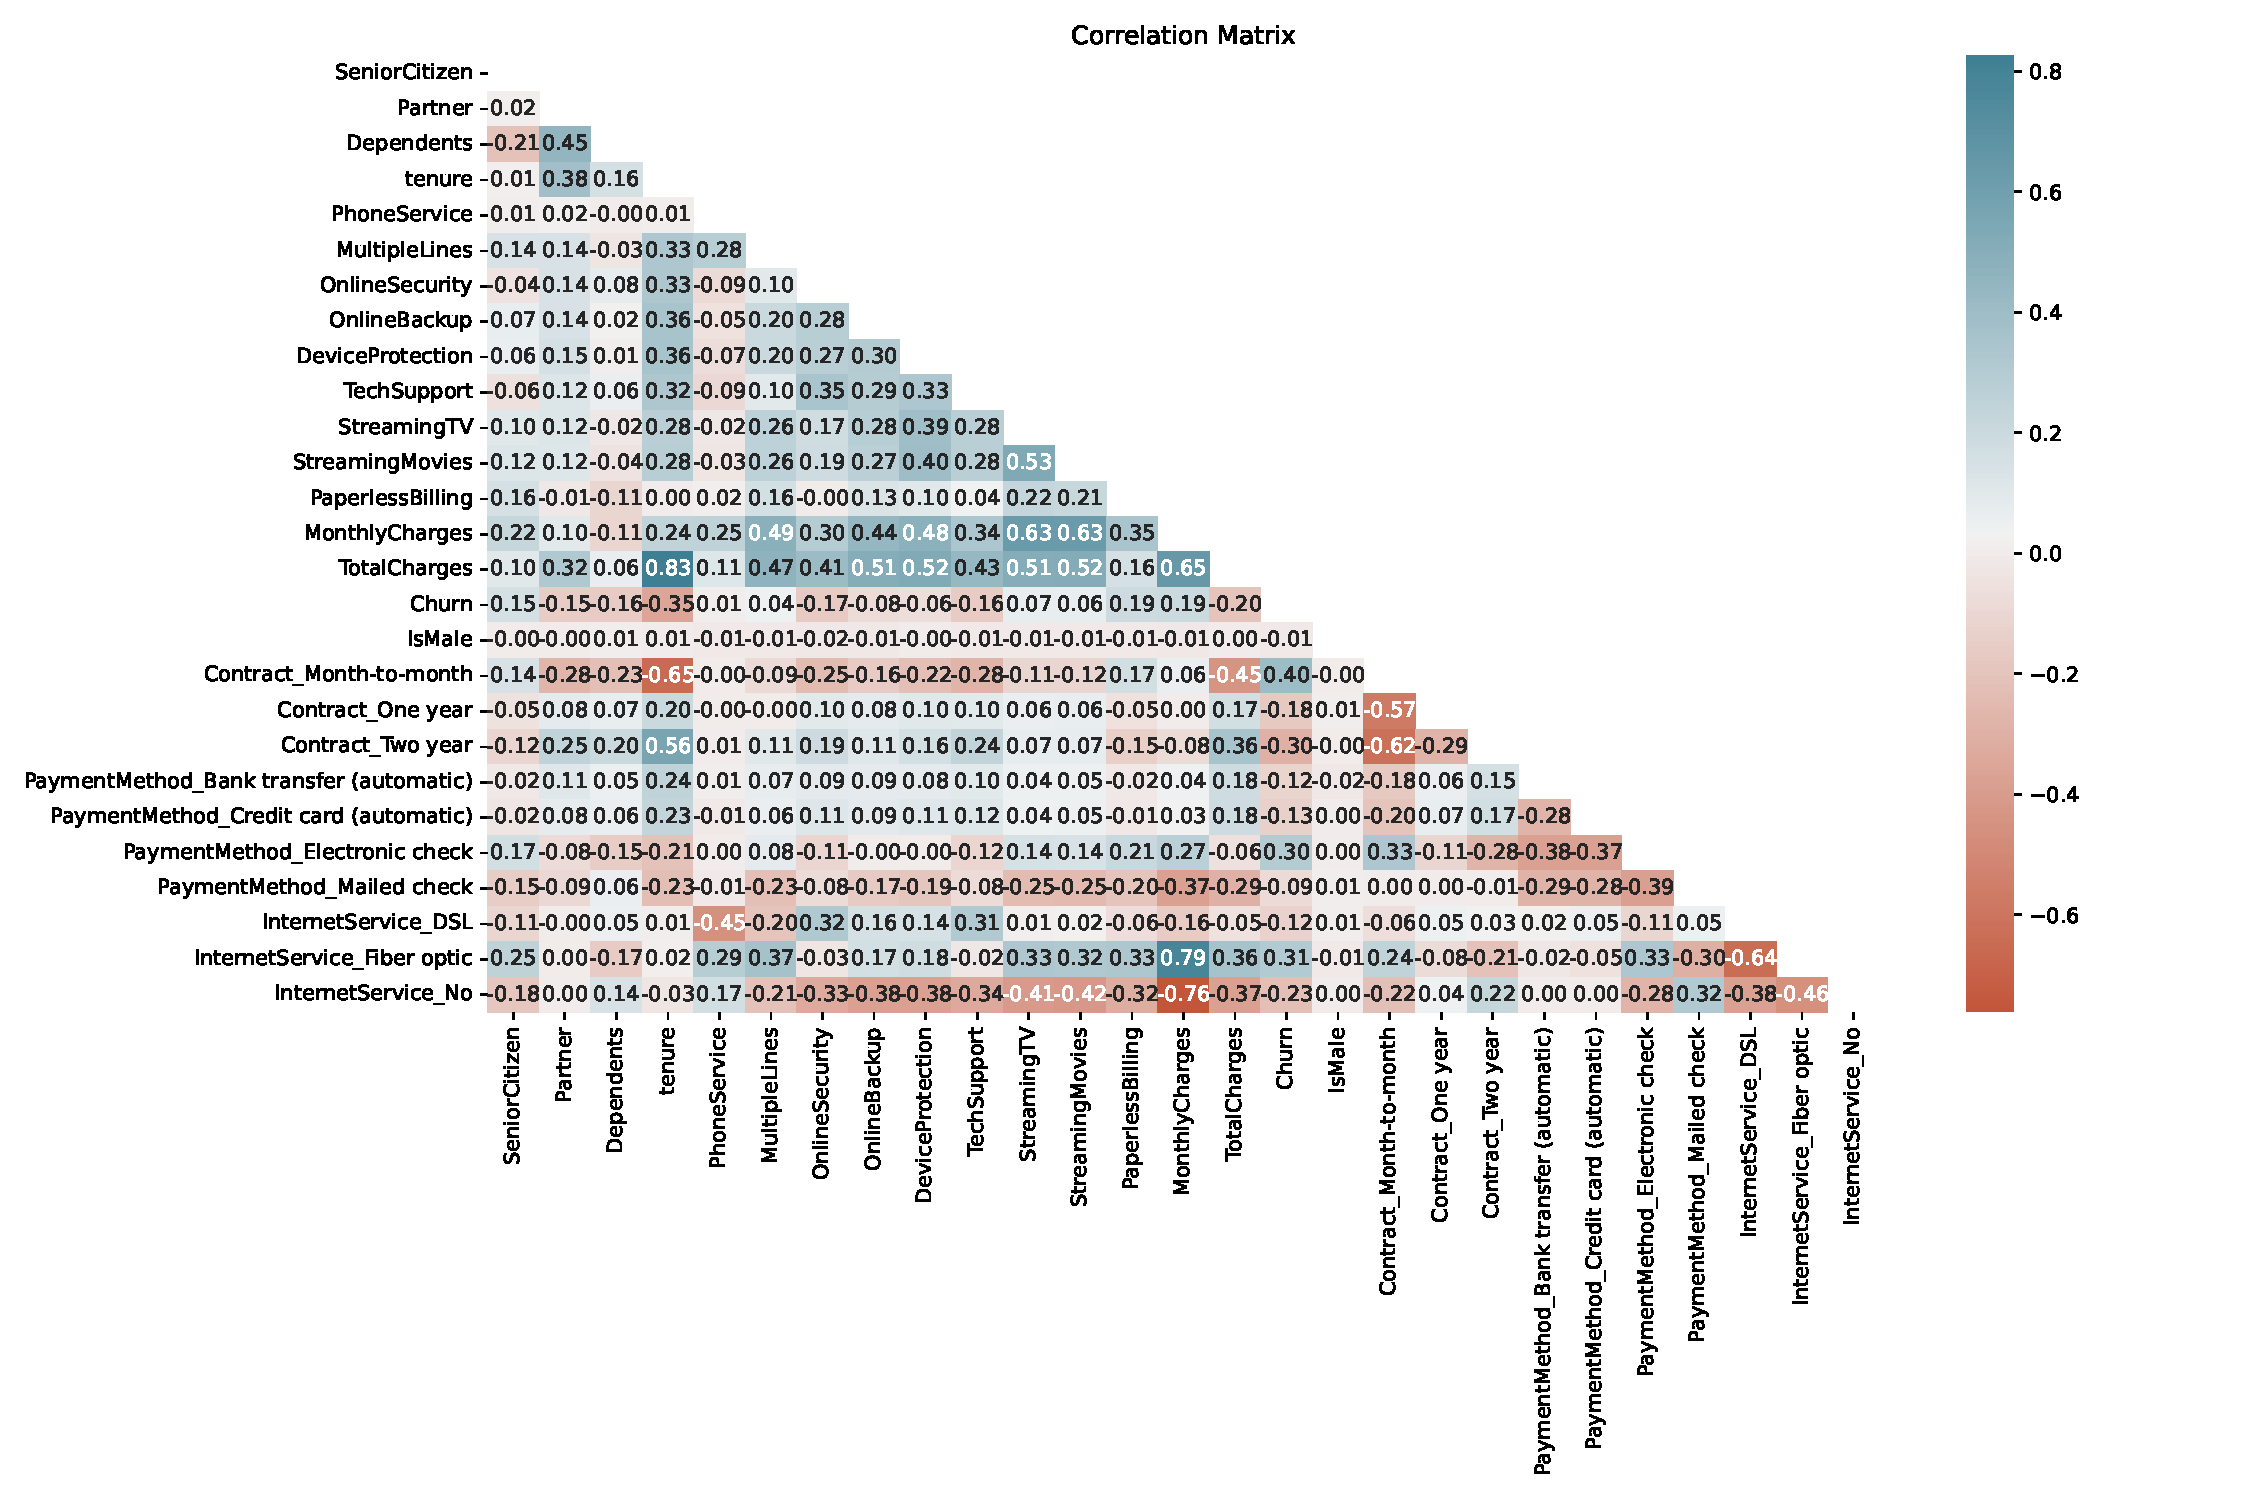
\includegraphics[width=\linewidth]{figures/understanding/correlation_matrix.pdf}
\caption{Correlation Heatmap}
\end{figure}
\begin{figure}[H]
\centering
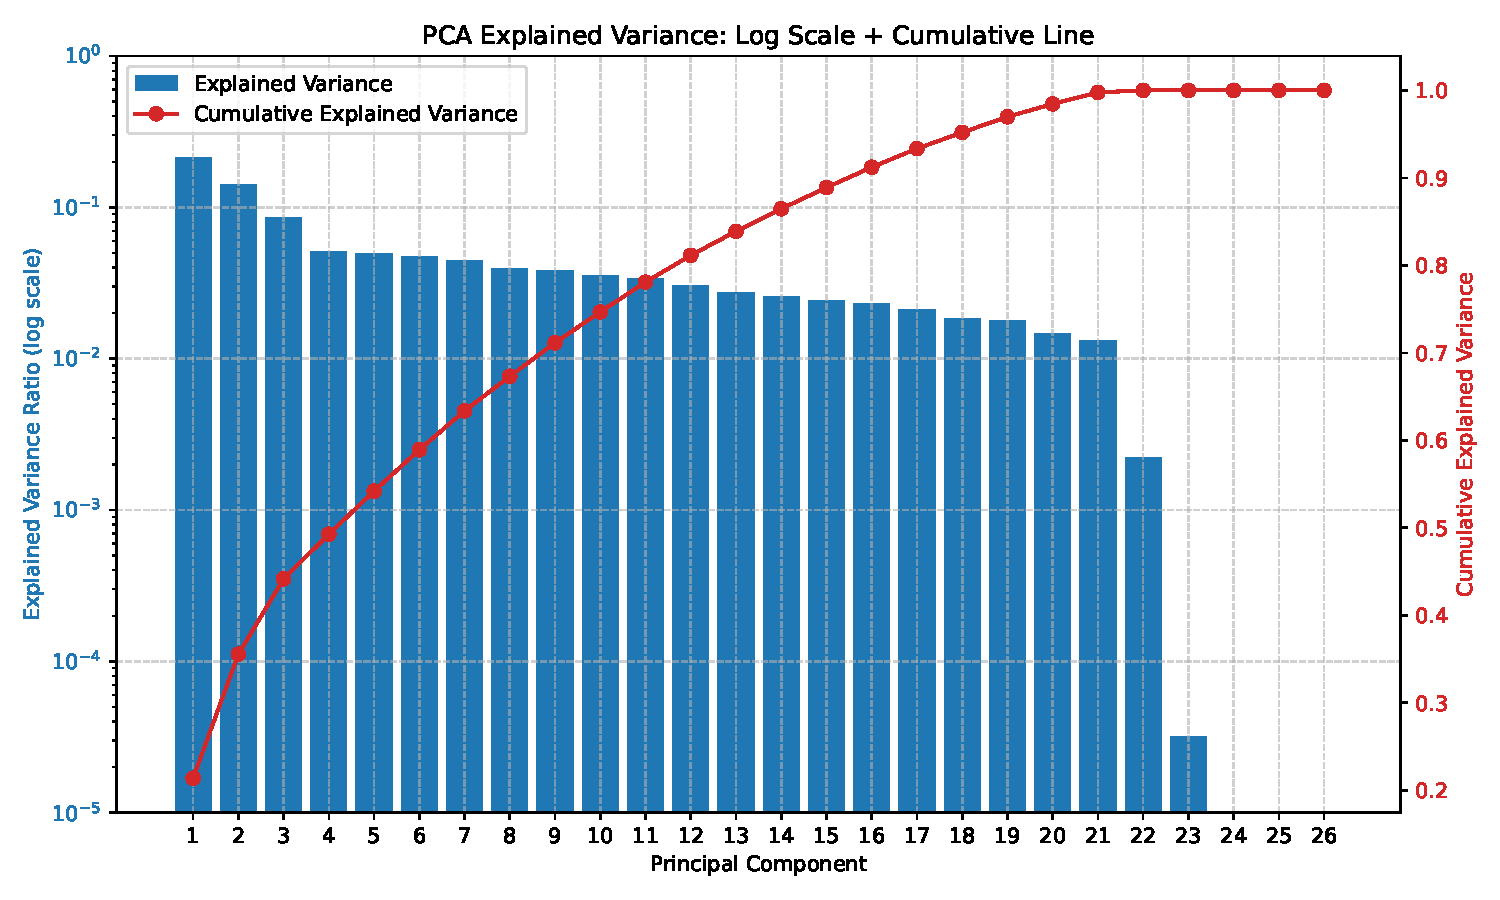
\includegraphics[width=0.8\linewidth]{figures/understanding/pca_explained_variance.pdf}
\caption{Normalized eigenvalues (explained variance by each component) and cumulative variance explained}
\label{fig:enter-label}
\end{figure}
\begin{table}
\centering
\adjustbox{max width=\textwidth}{%
\begin{tabular}{|r||c|c||c|c||c|c||c|c|}
\hline
& Predicted 1 & Predicted 0 & Predicted 1 & Predicted 0 & Predicted 1 & Predicted 0 & Predicted 1 & Predicted 0 \\\hline\hline
True 1 & \cellcolor{YellowGreen}273 & 186 & \cellcolor{YellowGreen}225 & 108 & \cellcolor{YellowGreen}176 & 54 & \cellcolor{YellowGreen}311 & 143 \\\cline{1-9}
True 0 & 165 & \cellcolor{Goldenrod}1129 & 213 & \cellcolor{Goldenrod}1207 & 262 & \cellcolor{Goldenrod}1261 & 246 & \cellcolor{Goldenrod}1403 \\\hline\hline
& \multicolumn{2}{|c||}{Decision Tree} & \multicolumn{2}{|c||}{Random Forest} &
\multicolumn{2}{|c||}{kNN} & \multicolumn{2}{|c|}{Logistic Regression} \\
\hline
\end{tabular}
}
\caption{Confusion matrices for classifying the target variable with different algorithms. Green indicates True Positives, yellow indicates True Negatives.}
\label{tab:conf_matrices}
\end{table}
\begin{figure}
\centering
\begin{subfigure}{0.49\linewidth}
    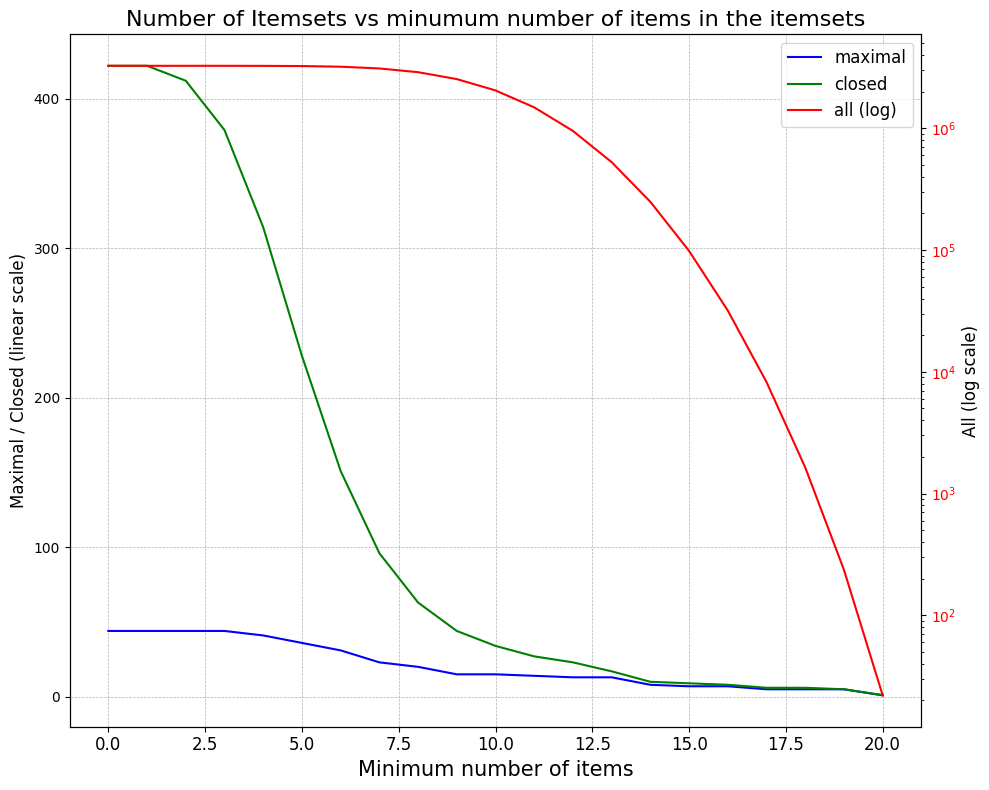
\includegraphics[width=\linewidth]{figures/pattern_mining/output.png}
\caption{Number of Frequent Itemsets with different minimum number of items required}
\label{fig:p}
\end{subfigure}
\begin{subfigure}{0.5\linewidth}
    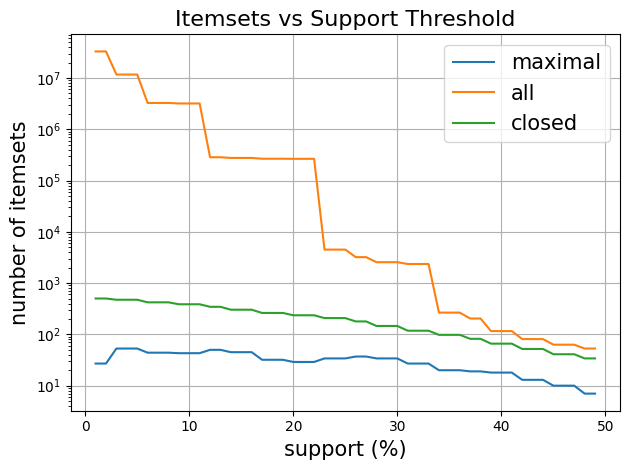
\includegraphics[width=\linewidth]{figures/pattern_mining/support.png}
\caption{Support}
\label{fig:sup}
\end{subfigure}
\caption{Number of Frequent Itemsets with different minimum requirements (support or number of items)}
\end{figure}

\begin{landscape}
\begin{figure}
\begin{subfigure}{0.14\linewidth}
    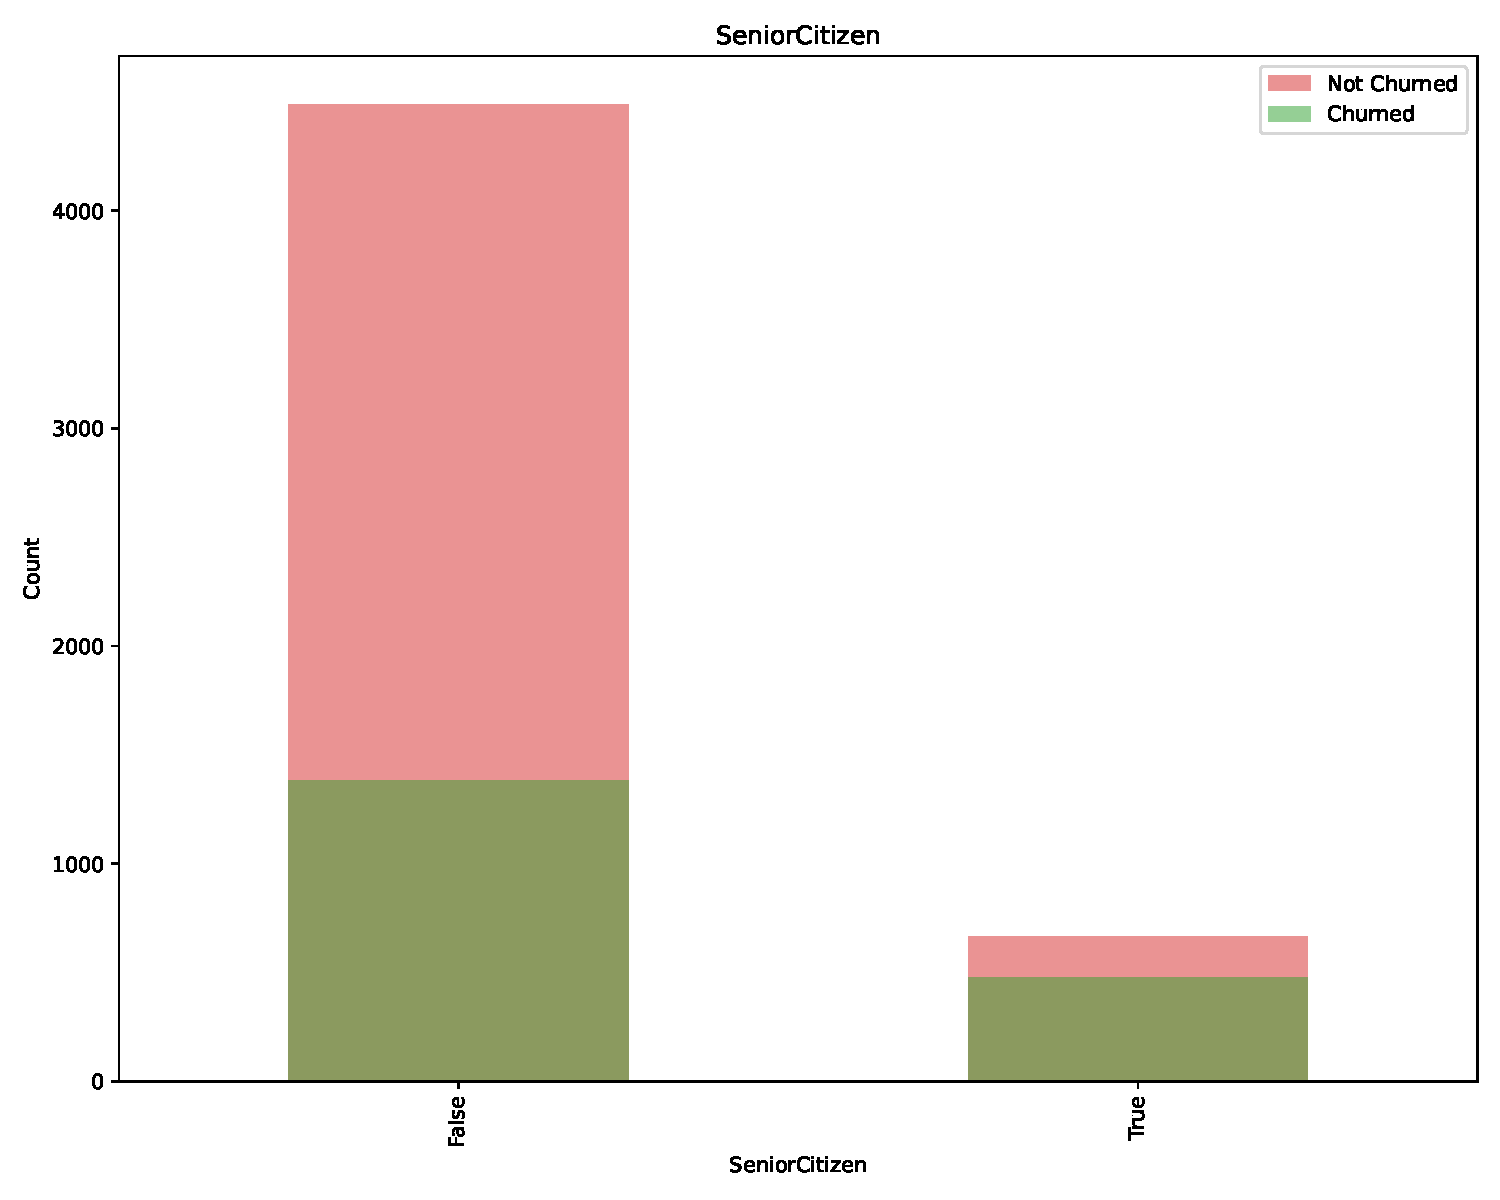
\includegraphics[width=\linewidth]{figures/understanding/SeniorCitizen.pdf}
    \caption{SeniorCitizen}
\end{subfigure}%
\begin{subfigure}{0.14\linewidth}
    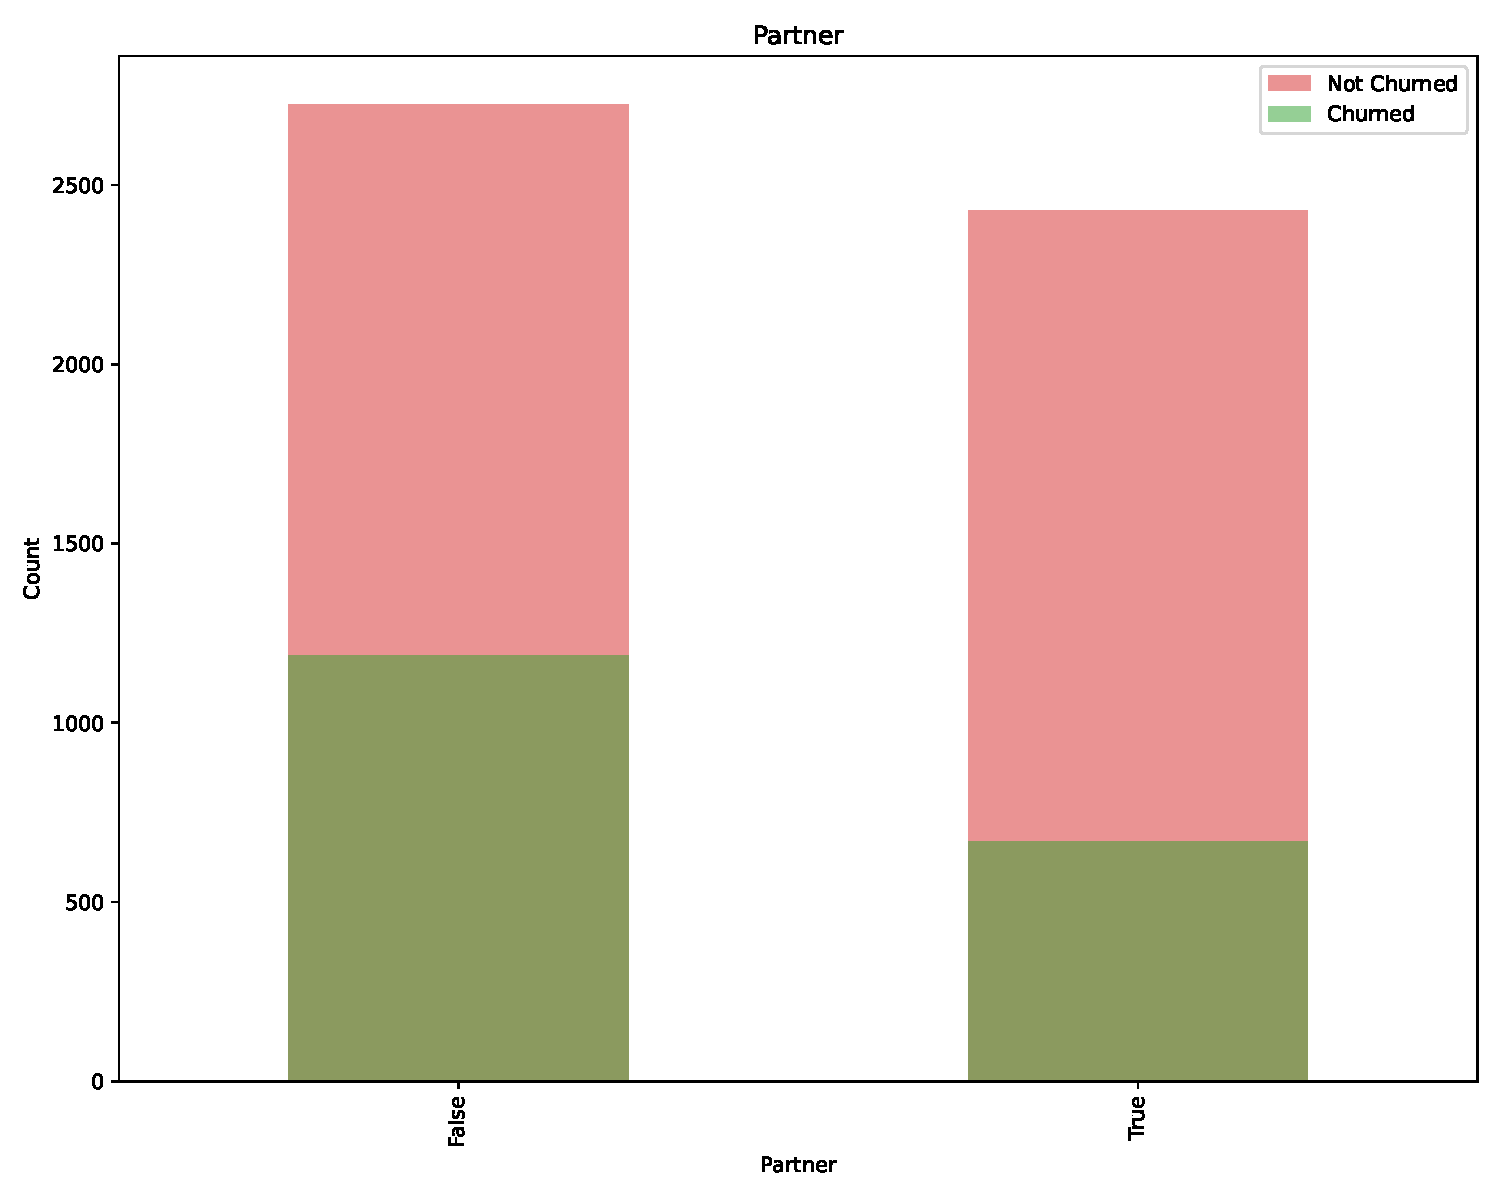
\includegraphics[width=\linewidth]{figures/understanding/Partner.pdf}
    \caption{Partner}
    \end{subfigure}
\begin{subfigure}{0.14\linewidth}
    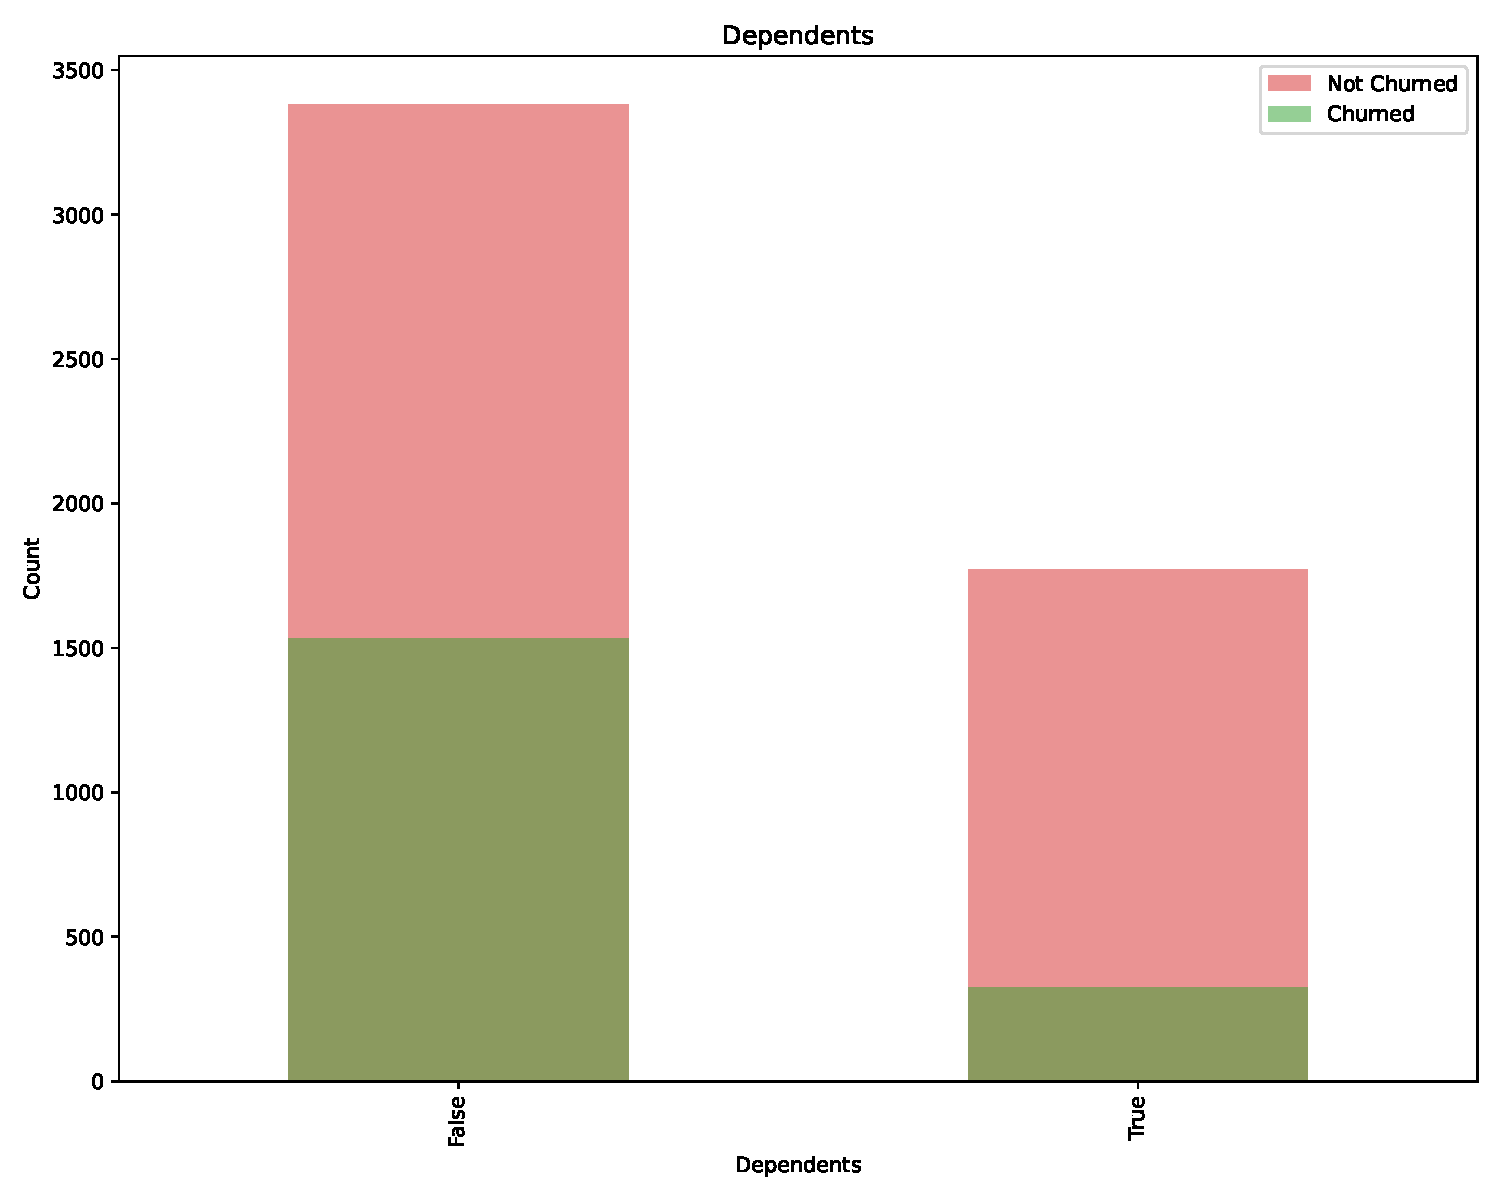
\includegraphics[width=\linewidth]{figures/understanding/Dependents.pdf}
    \caption{Dependents}
\end{subfigure}
\begin{subfigure}{0.14\linewidth}
    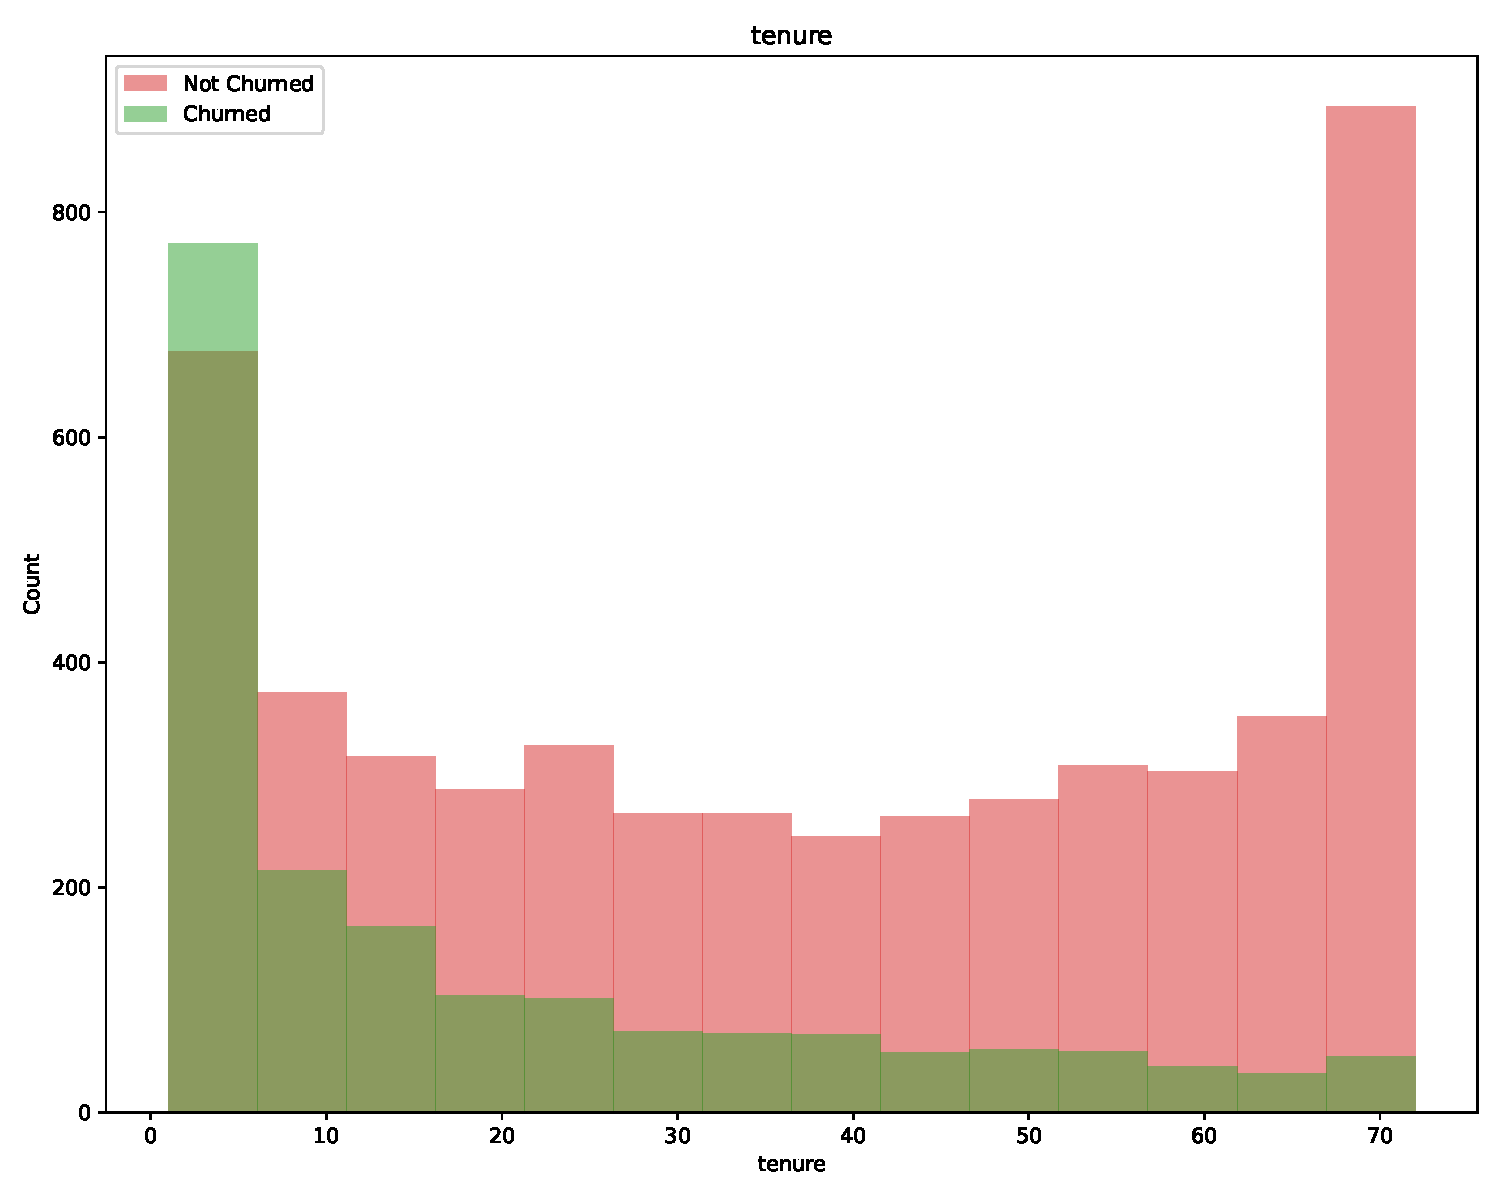
\includegraphics[width=\linewidth]{figures/understanding/tenure.pdf}
    \caption{Tenure}
\end{subfigure}
\begin{subfigure}{0.14\linewidth}
    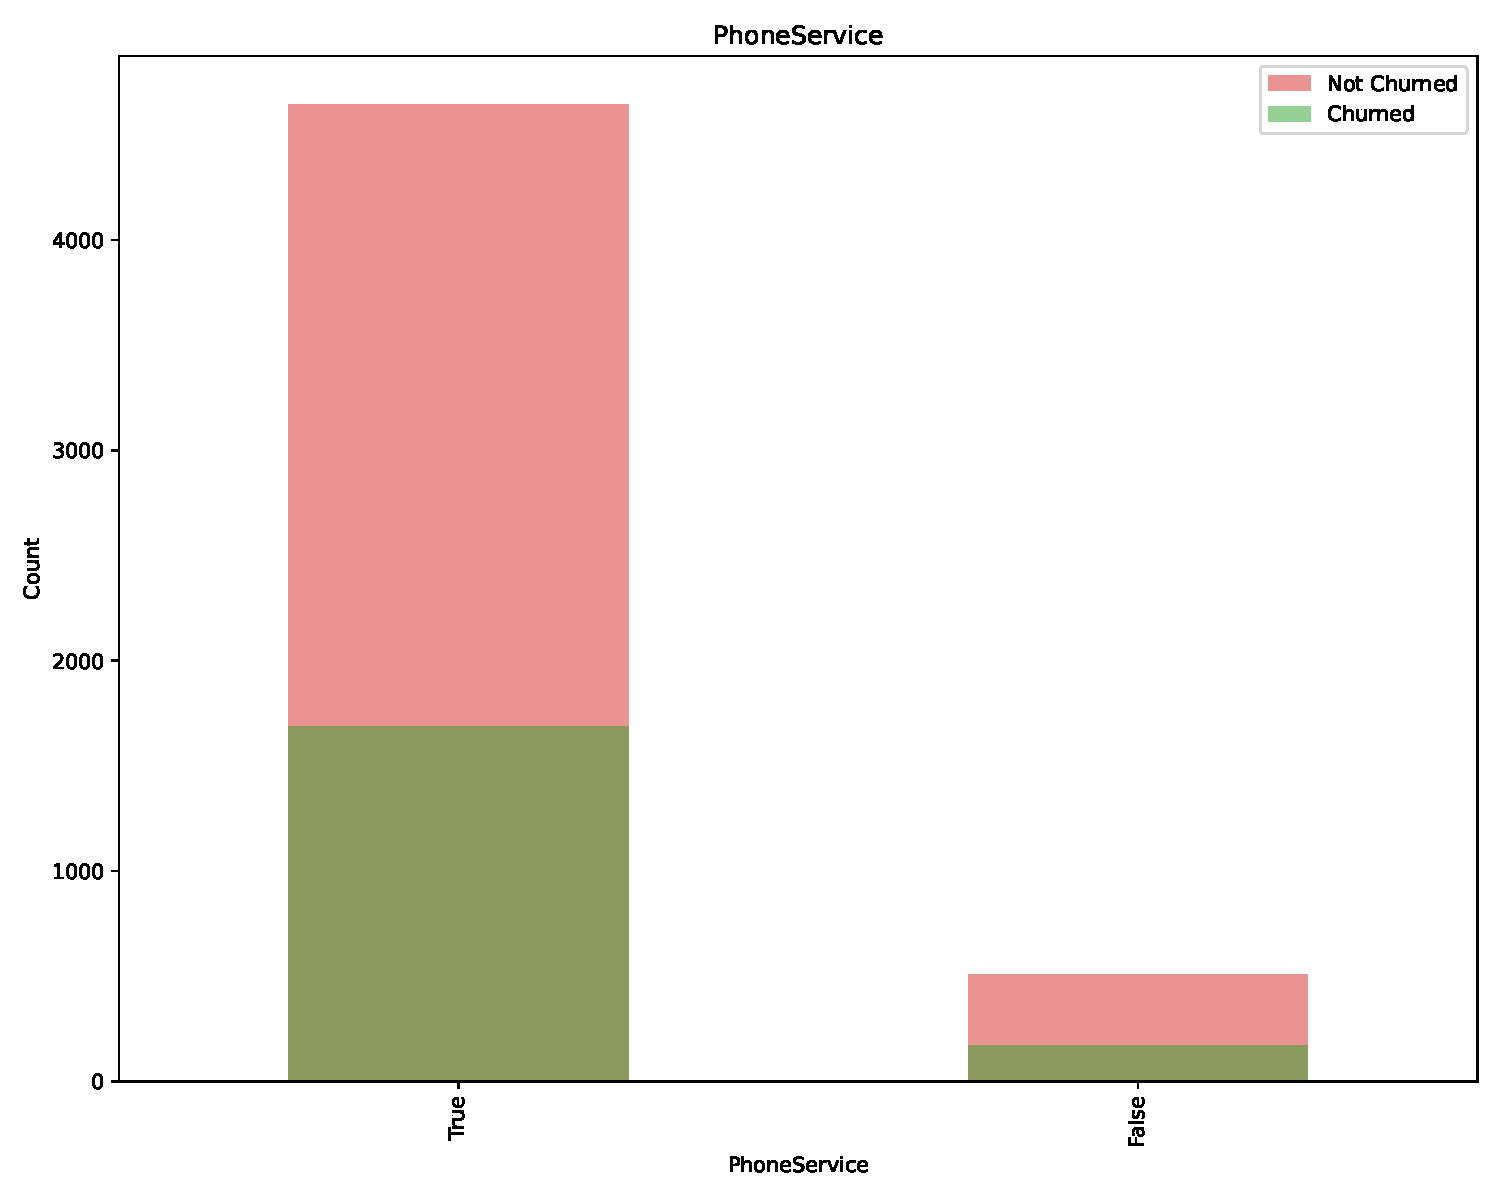
\includegraphics[width=\linewidth]{figures/understanding/PhoneService.pdf}
    \caption{PhoneService}
\end{subfigure}
\begin{subfigure}{0.14\linewidth}
    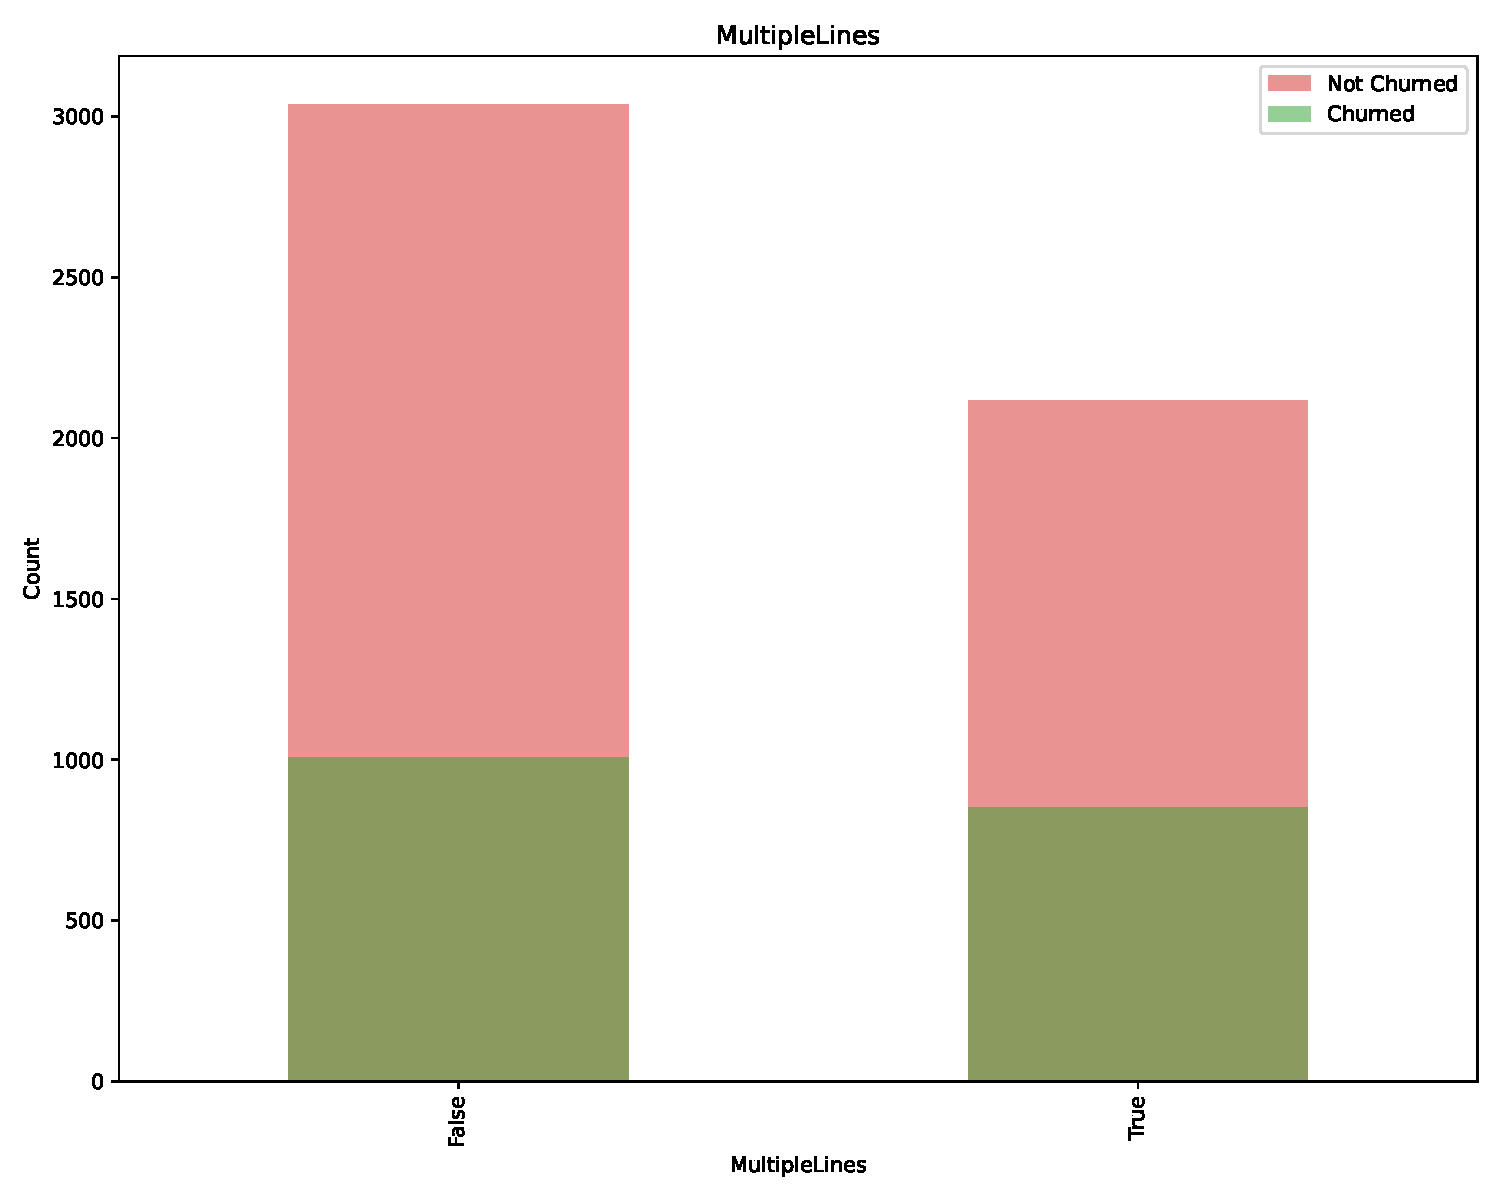
\includegraphics[width=\linewidth]{figures/understanding/MultipleLines.pdf}
    \caption{MultipleLines}
\end{subfigure}
\begin{subfigure}{0.14\linewidth}
    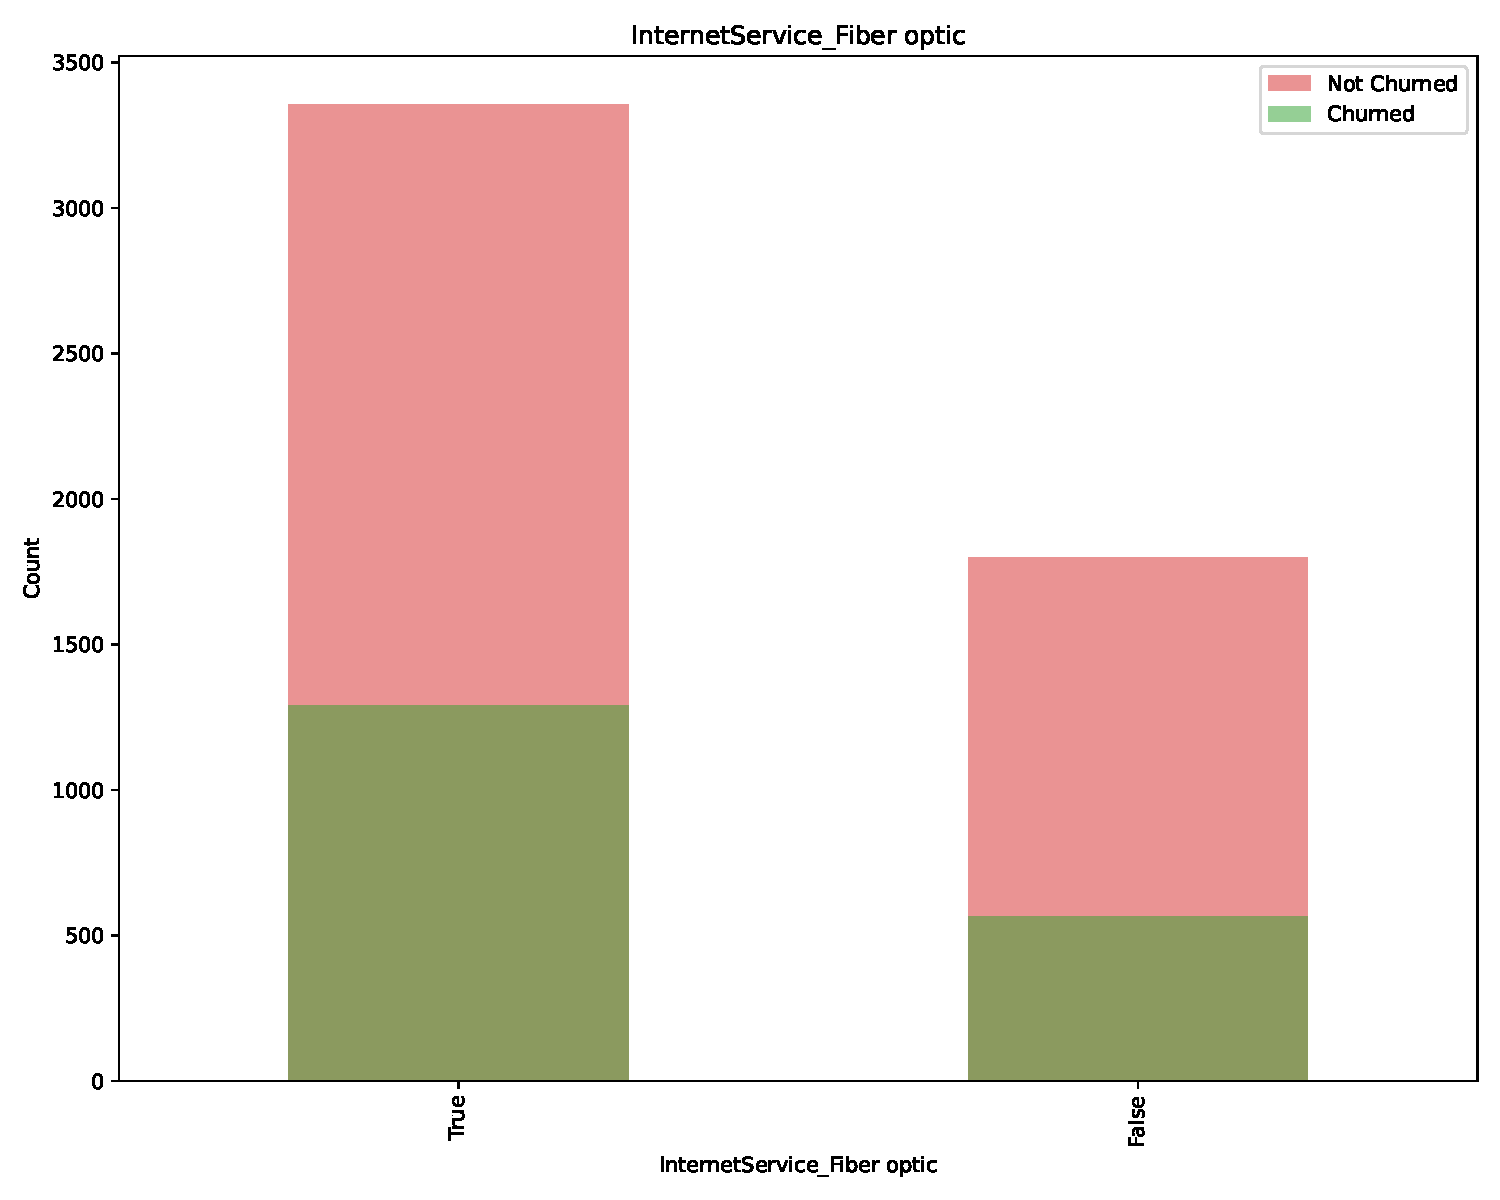
\includegraphics[width=\linewidth]{figures/understanding/InternetService_Fiber optic.pdf}
    \caption{InternetService [Fiber Optic]}
\end{subfigure}

\begin{subfigure}{0.13\linewidth}
    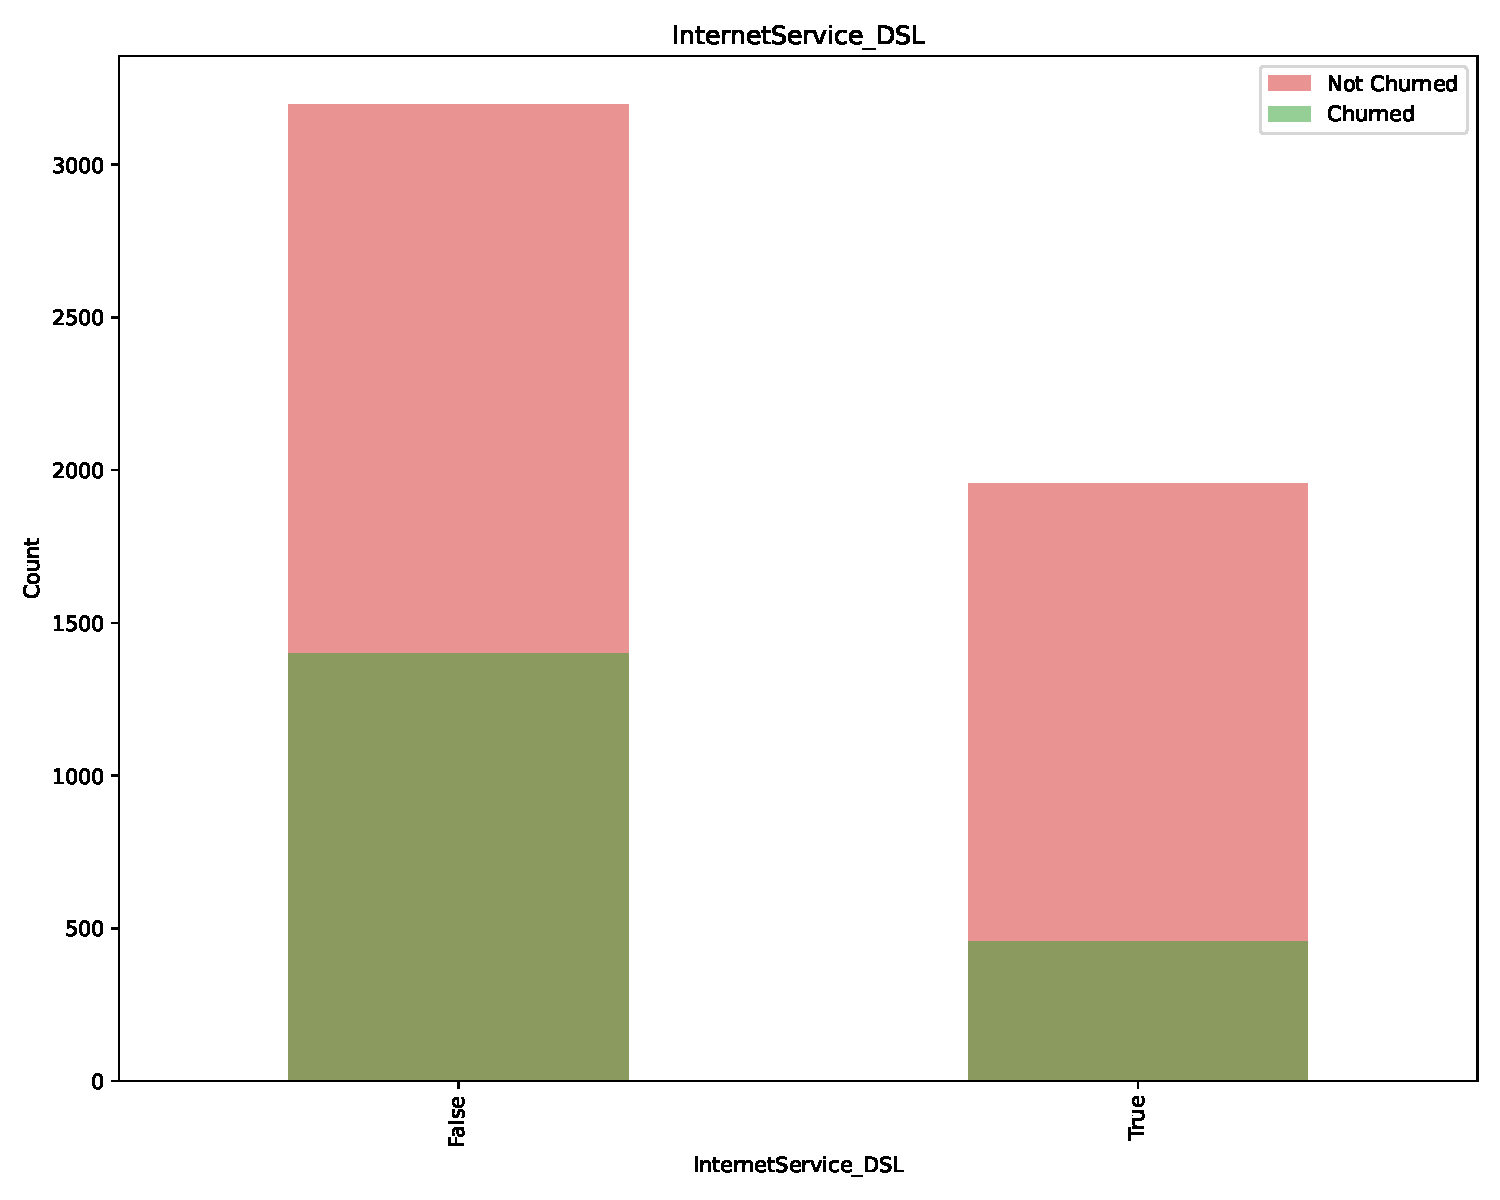
\includegraphics[width=\linewidth]{figures/understanding/InternetService_DSL.pdf}
    \caption{InternetService [DSL]}
\end{subfigure}
\begin{subfigure}{0.14\linewidth}
    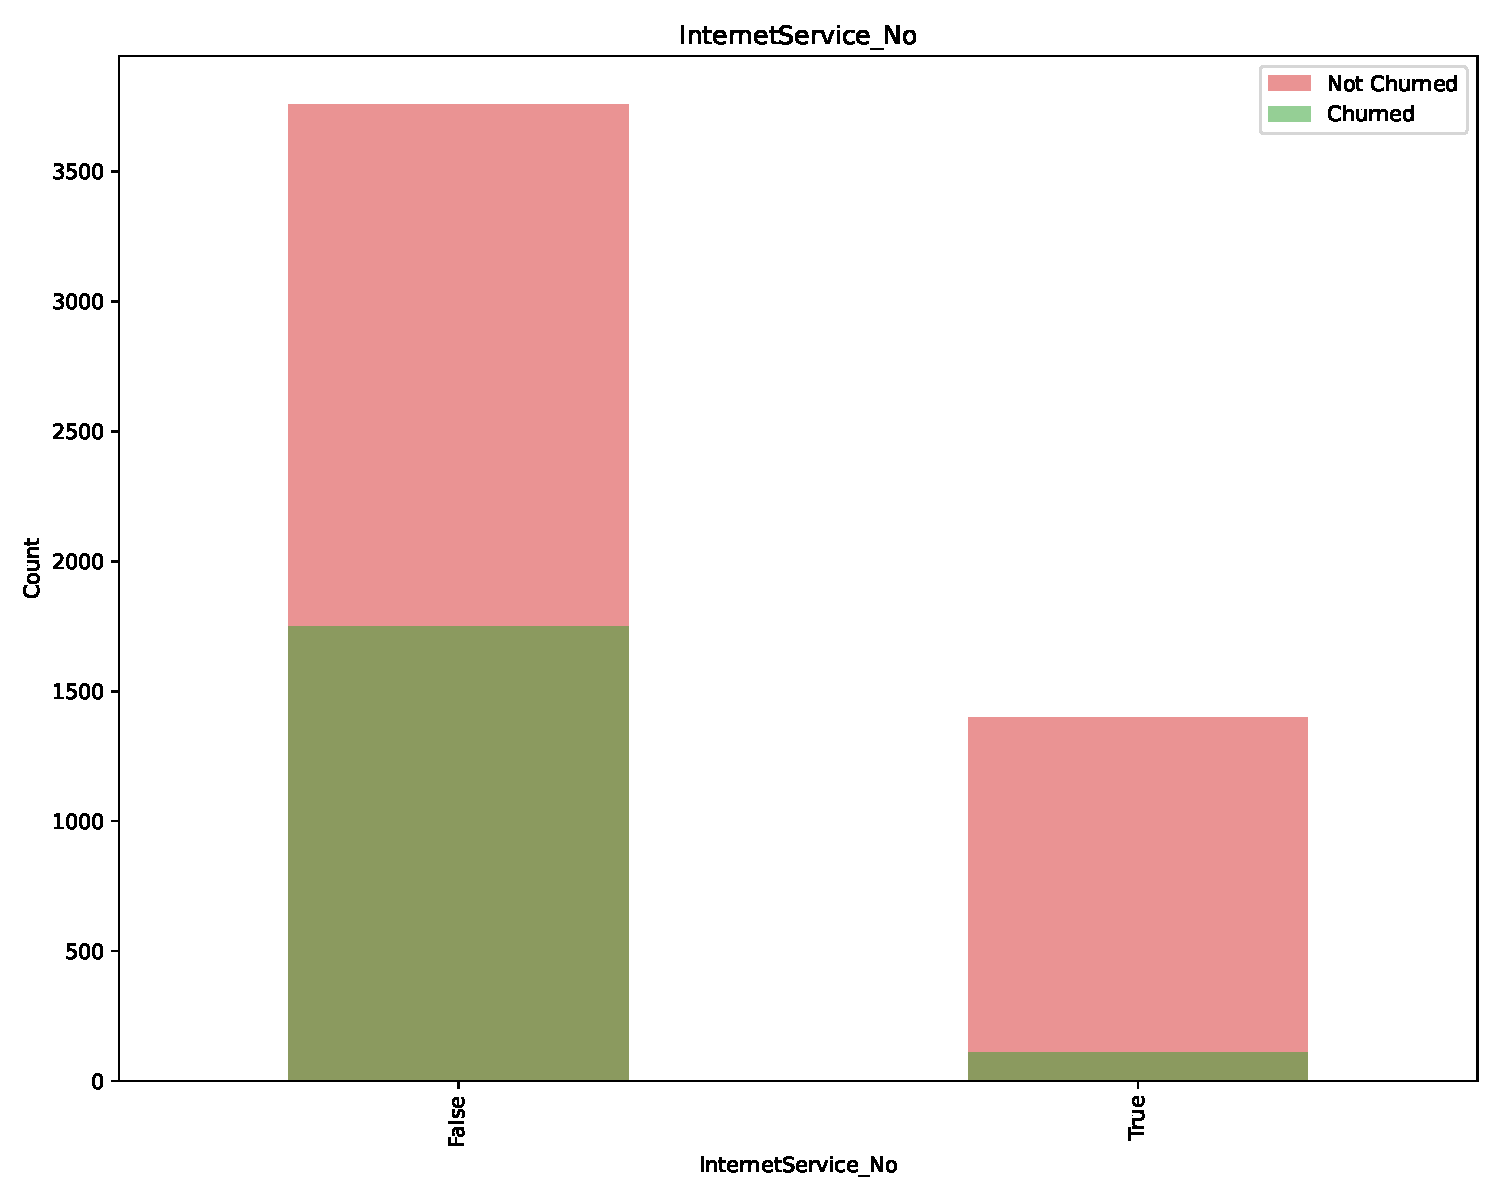
\includegraphics[width=\linewidth]{figures/understanding/InternetService_No.pdf}
    \caption{InternetService [No]}
\end{subfigure}
\begin{subfigure}{0.14\linewidth}
    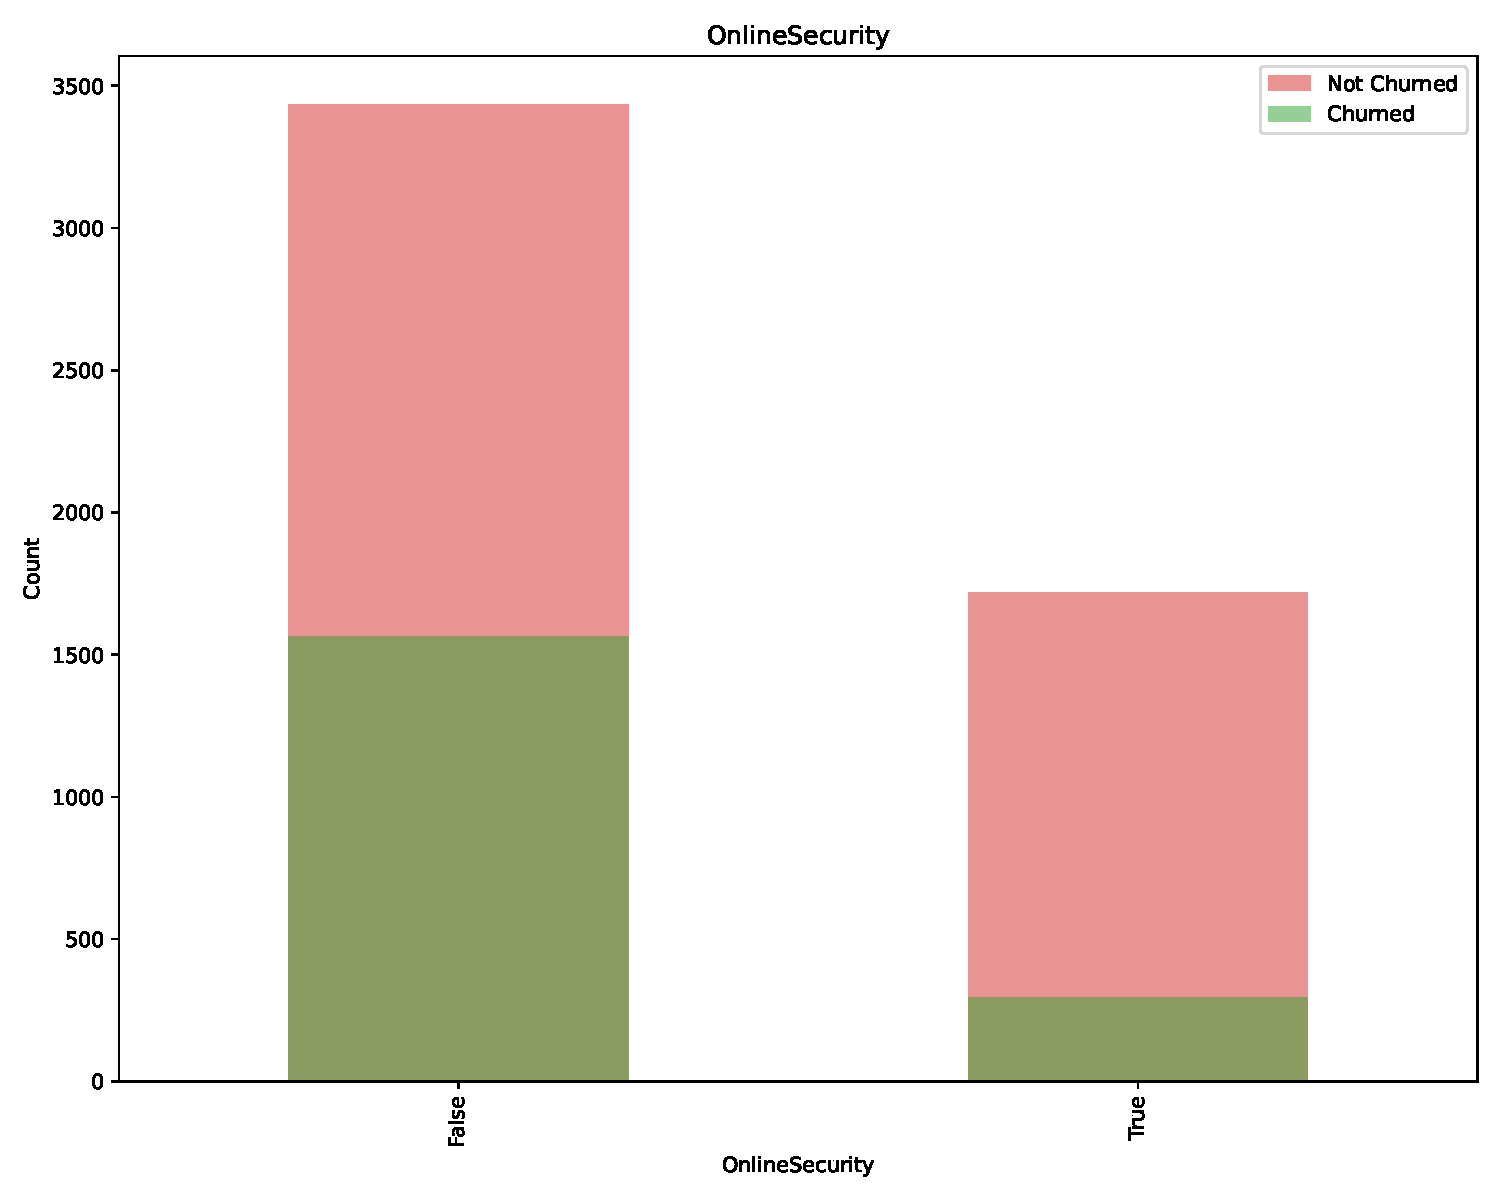
\includegraphics[width=\linewidth]{figures/understanding/OnlineSecurity.pdf}
    \caption{OnlineSecurity}
\end{subfigure}
\begin{subfigure}{0.14\linewidth}
    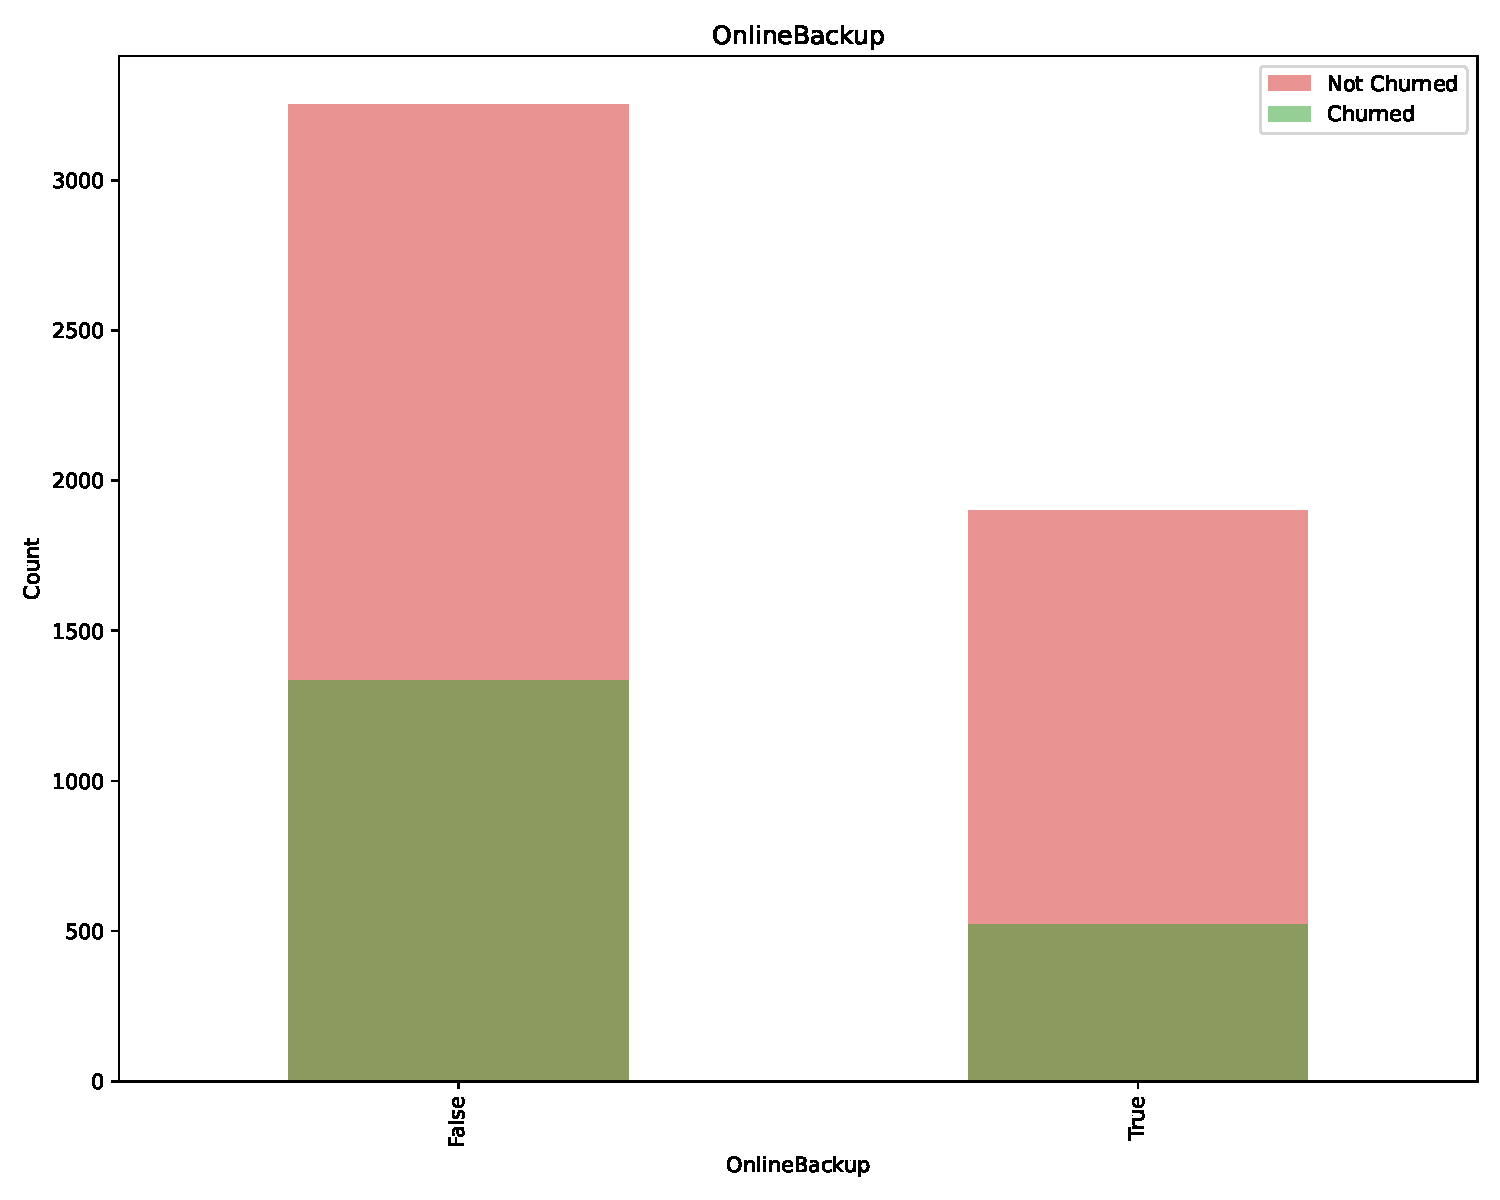
\includegraphics[width=\linewidth]{figures/understanding/OnlineBackup.pdf}
    \caption{OnlineBackup}
\end{subfigure}
\begin{subfigure}{0.14\linewidth}
    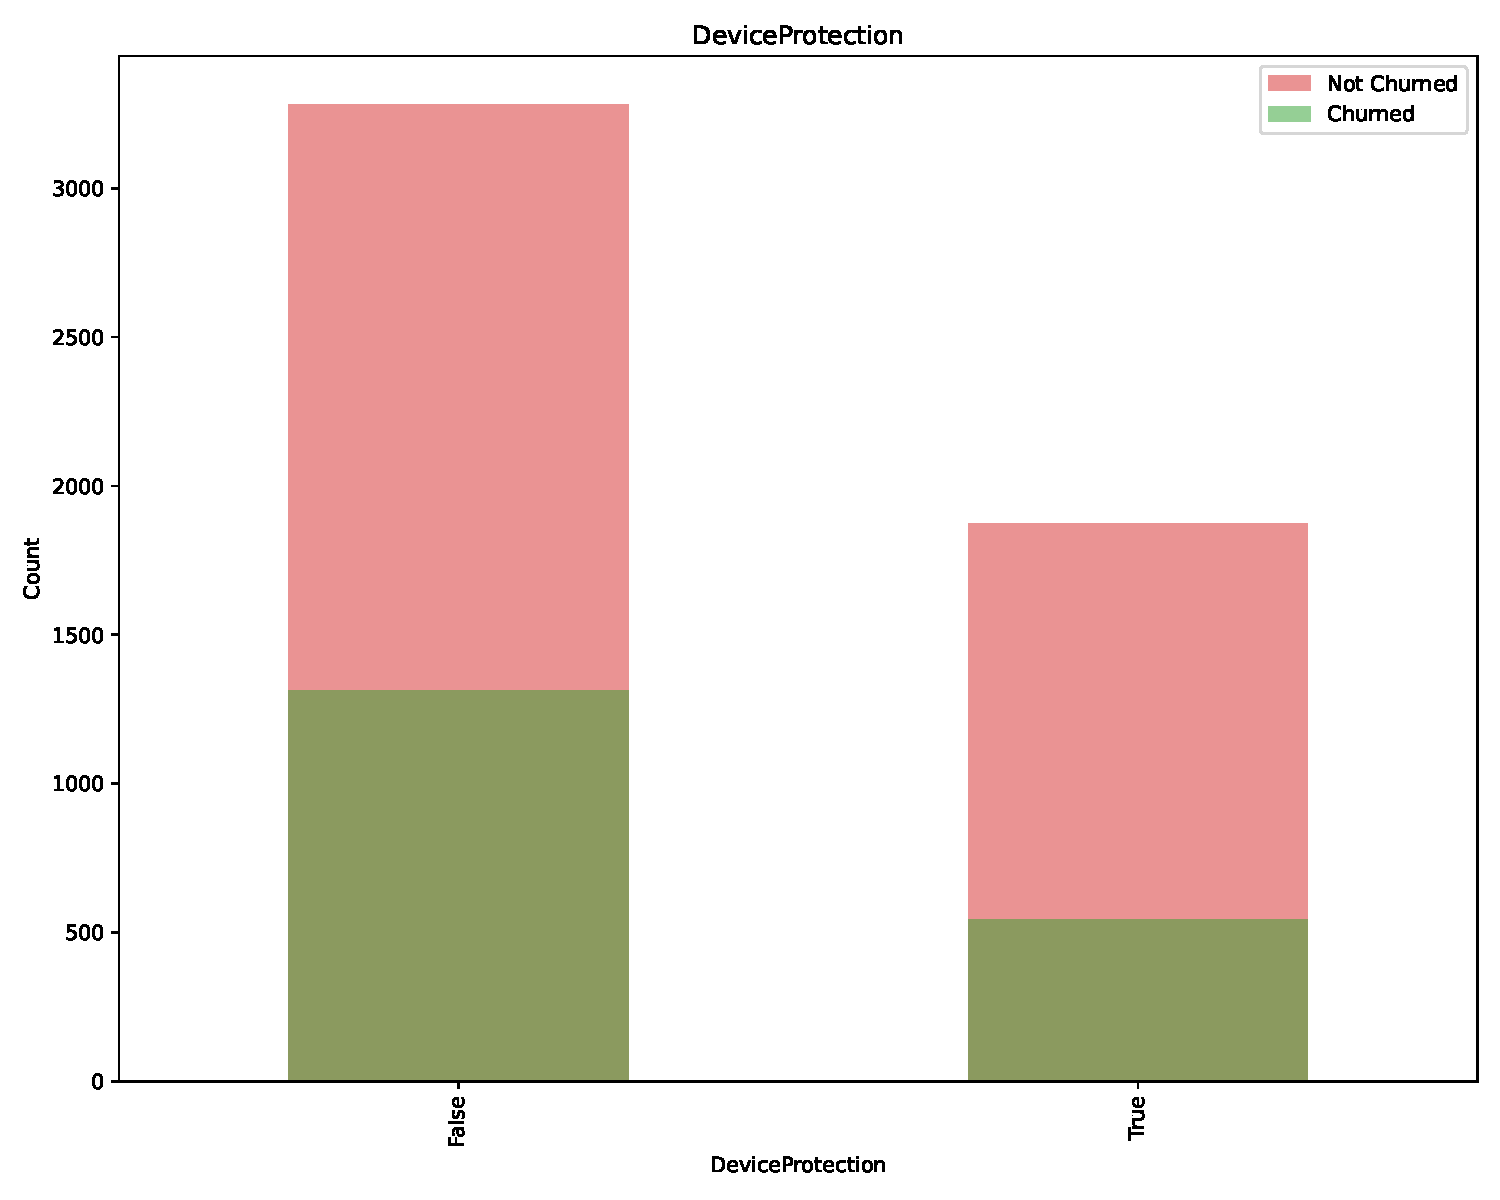
\includegraphics[width=\linewidth]{figures/understanding/DeviceProtection.pdf}
    \caption{DeviceProtection}
\end{subfigure}
\begin{subfigure}{0.14\linewidth}
    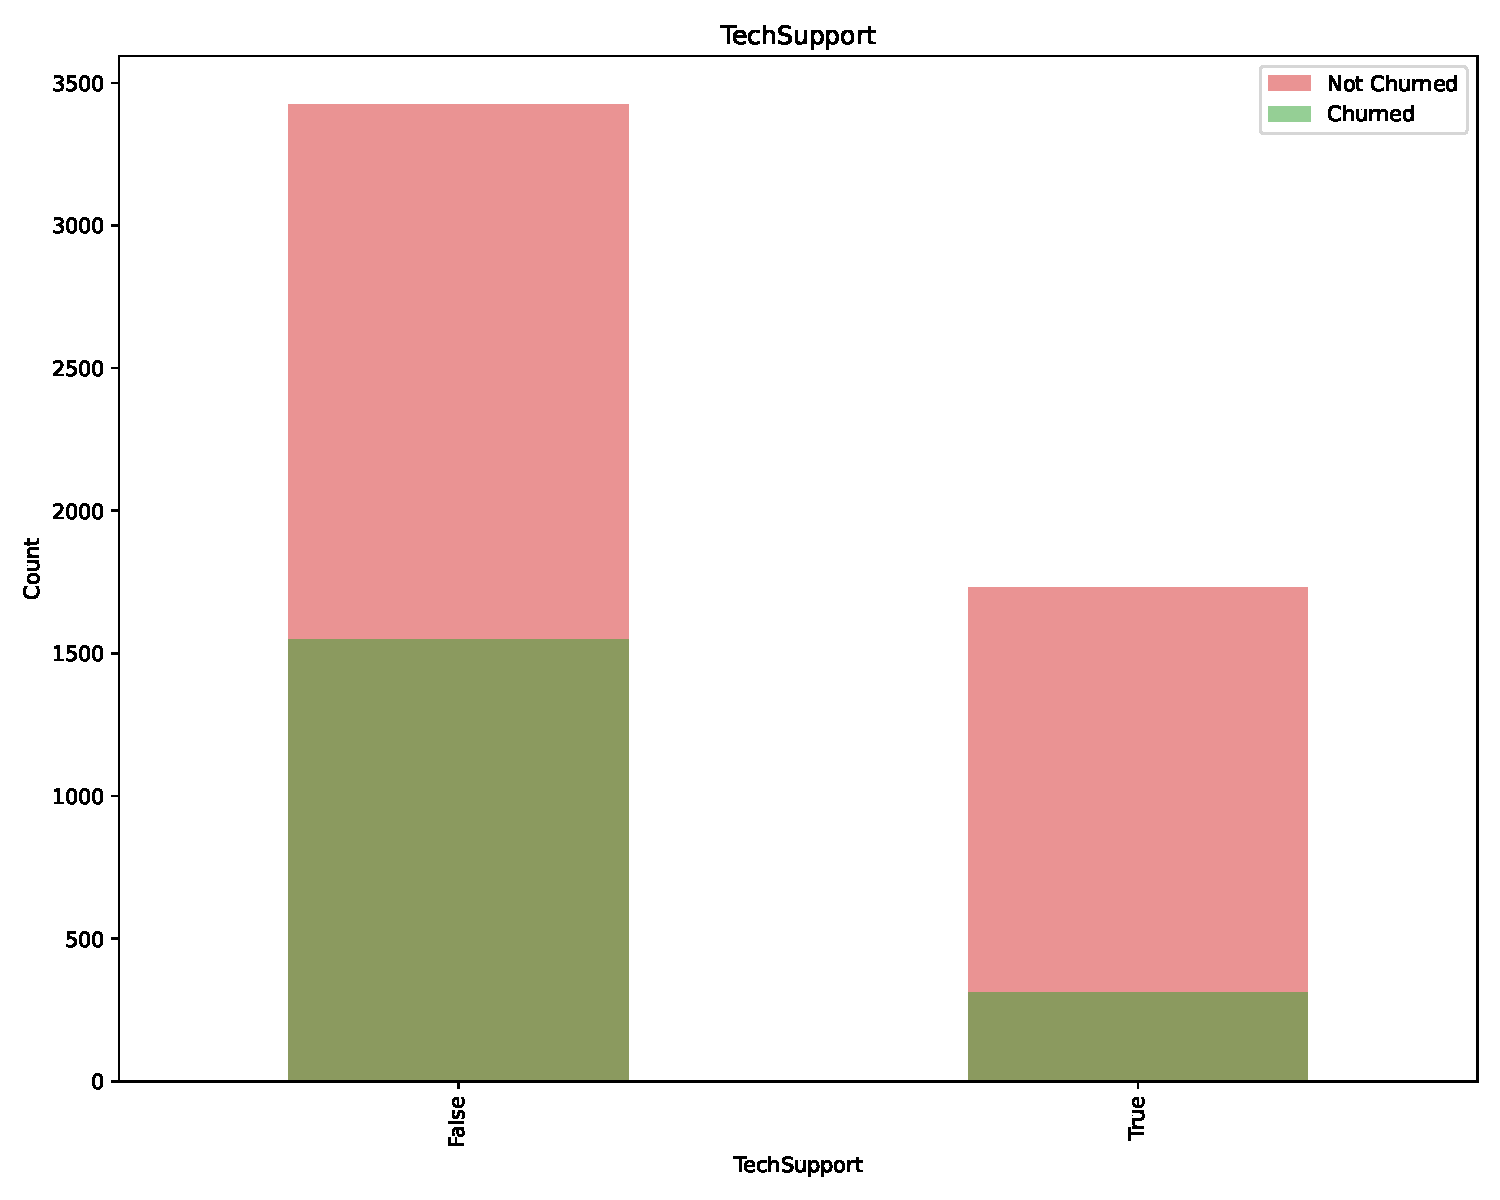
\includegraphics[width=\linewidth]{figures/understanding/TechSupport.pdf}
    \caption{TechSupport}
\end{subfigure}
\begin{subfigure}{0.14\linewidth}
    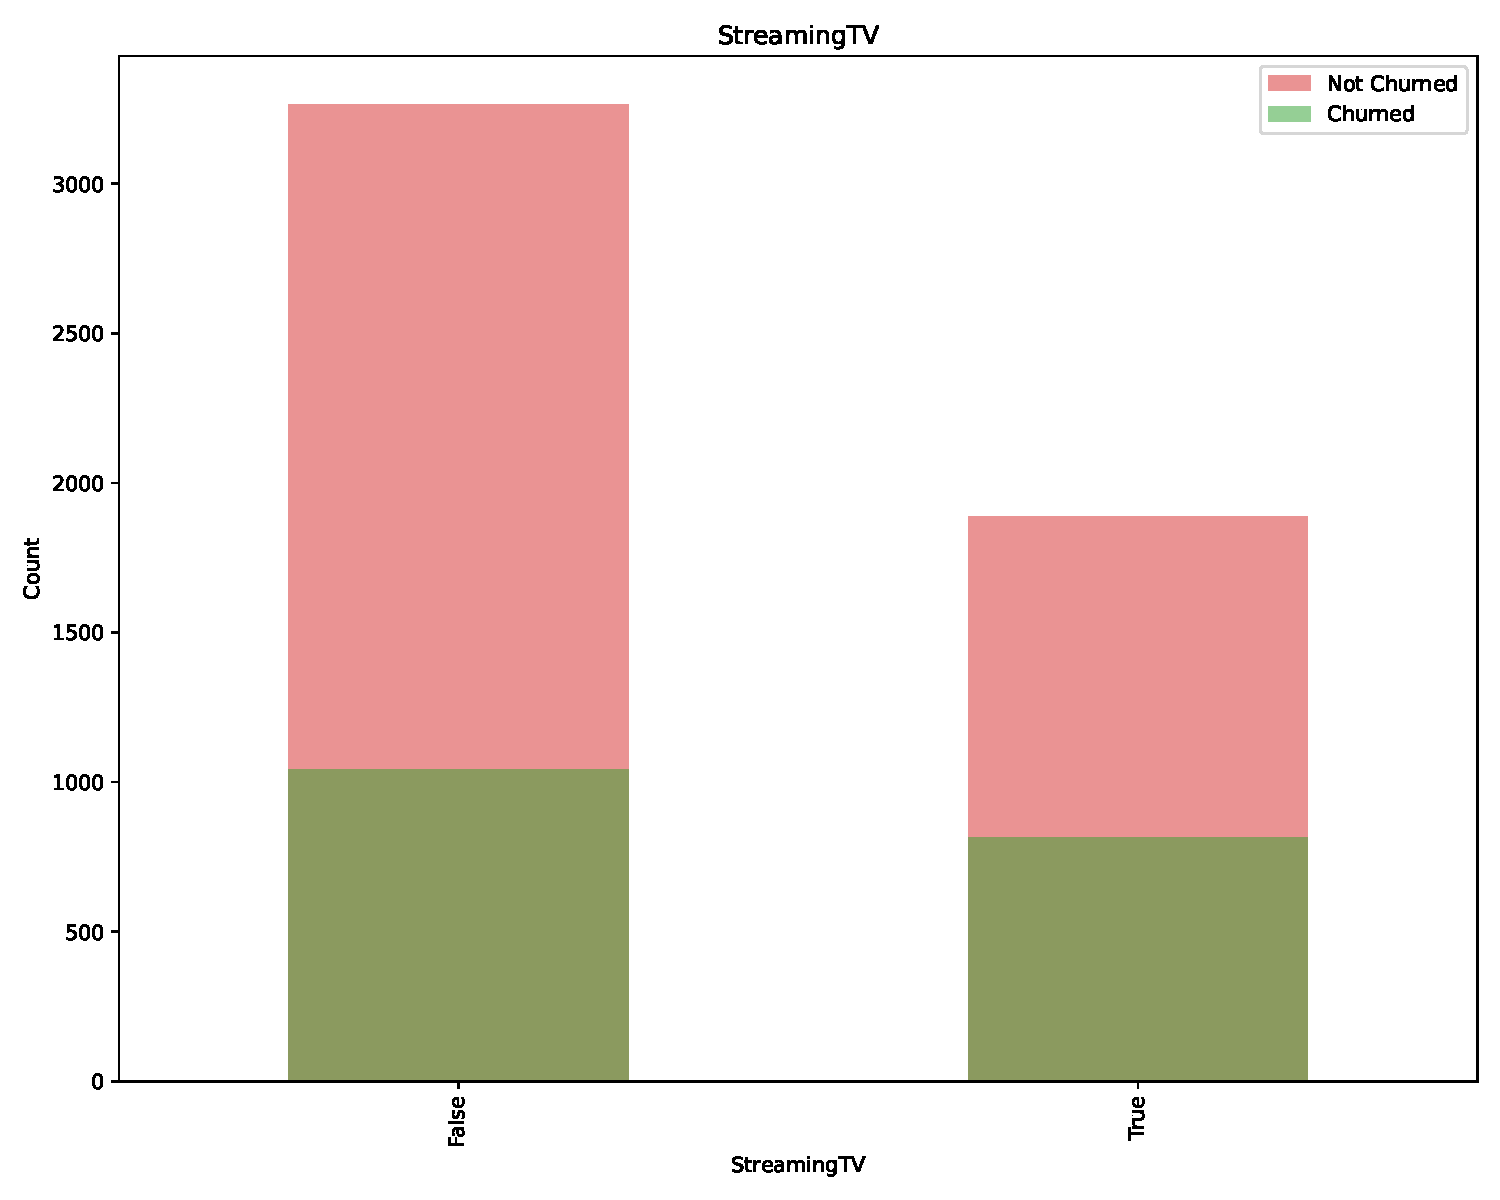
\includegraphics[width=\linewidth]{figures/understanding/StreamingTV.pdf}
    \caption{StreamingTV}
\end{subfigure}

\begin{subfigure}{0.14\linewidth}
    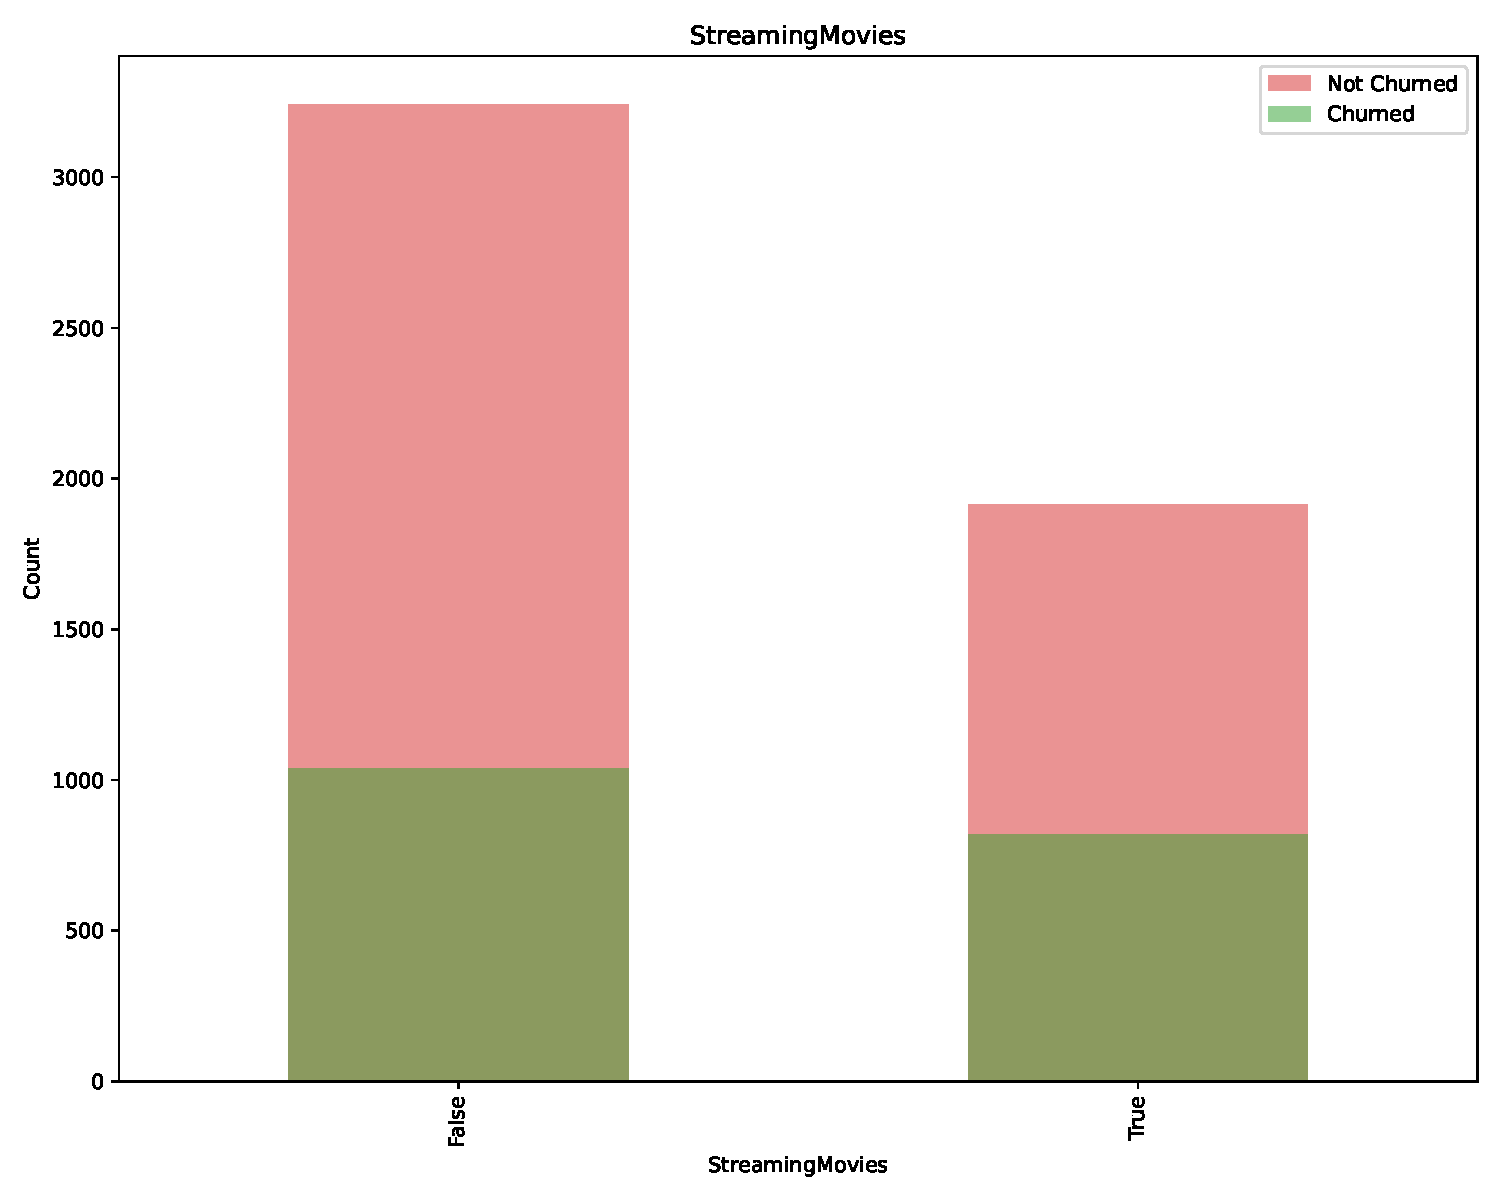
\includegraphics[width=\linewidth]{figures/understanding/StreamingMovies.pdf}
    \caption{StreamingMovies}
\end{subfigure}
\begin{subfigure}{0.14\linewidth}
    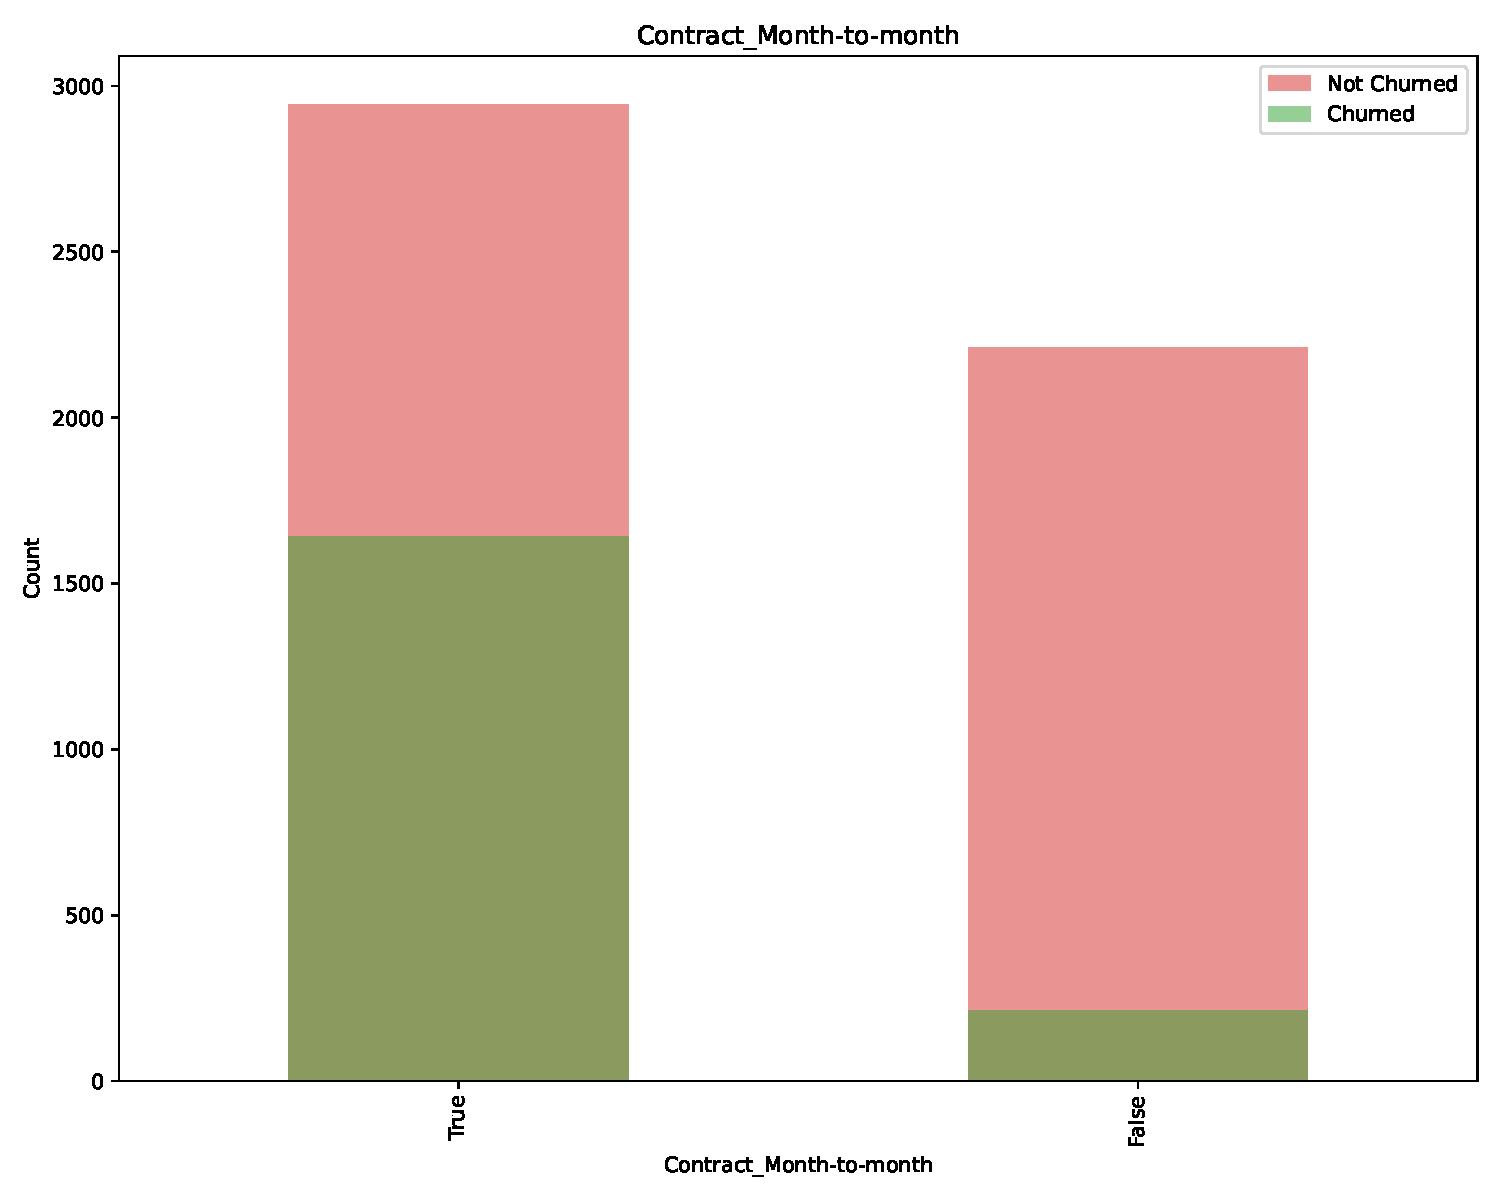
\includegraphics[width=\linewidth]{figures/understanding/Contract_Month-to-month.pdf}
    \caption{Contract [Month-to-Month]}
\end{subfigure}
\begin{subfigure}{0.14\linewidth}
    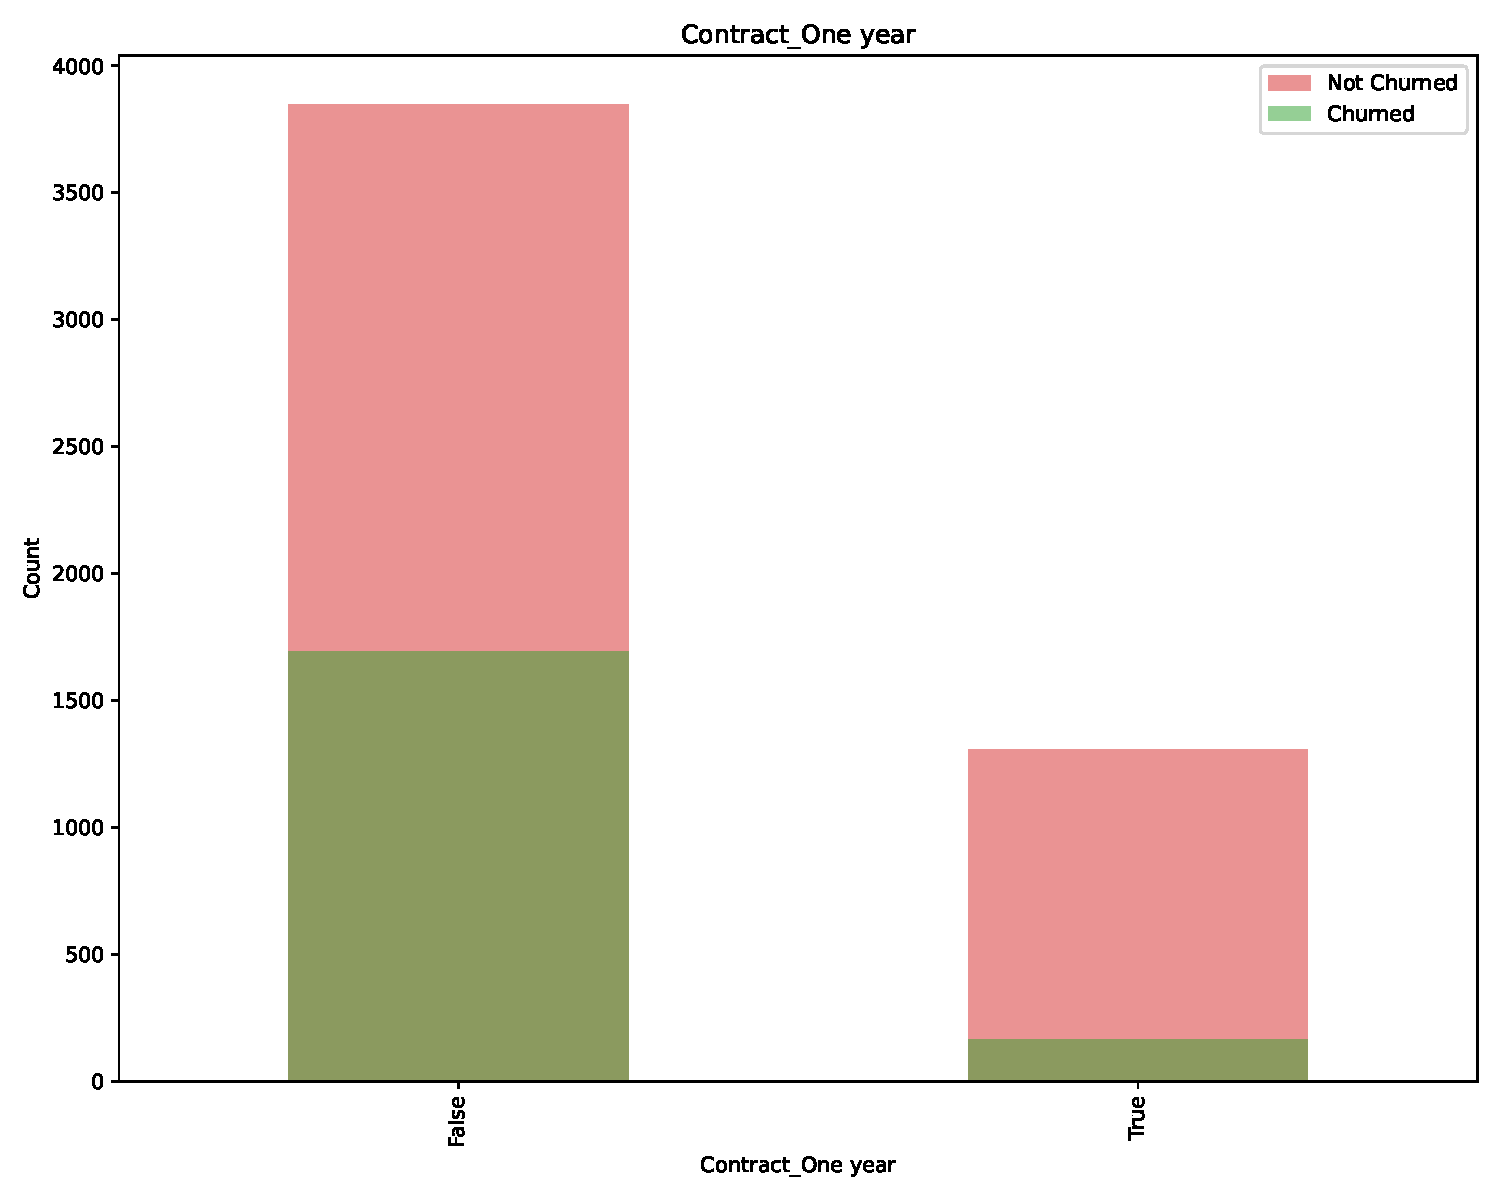
\includegraphics[width=\linewidth]{figures/understanding/Contract_One year.pdf}
    \caption{Contract [One-Year]}
\end{subfigure}
\begin{subfigure}{0.14\linewidth}
    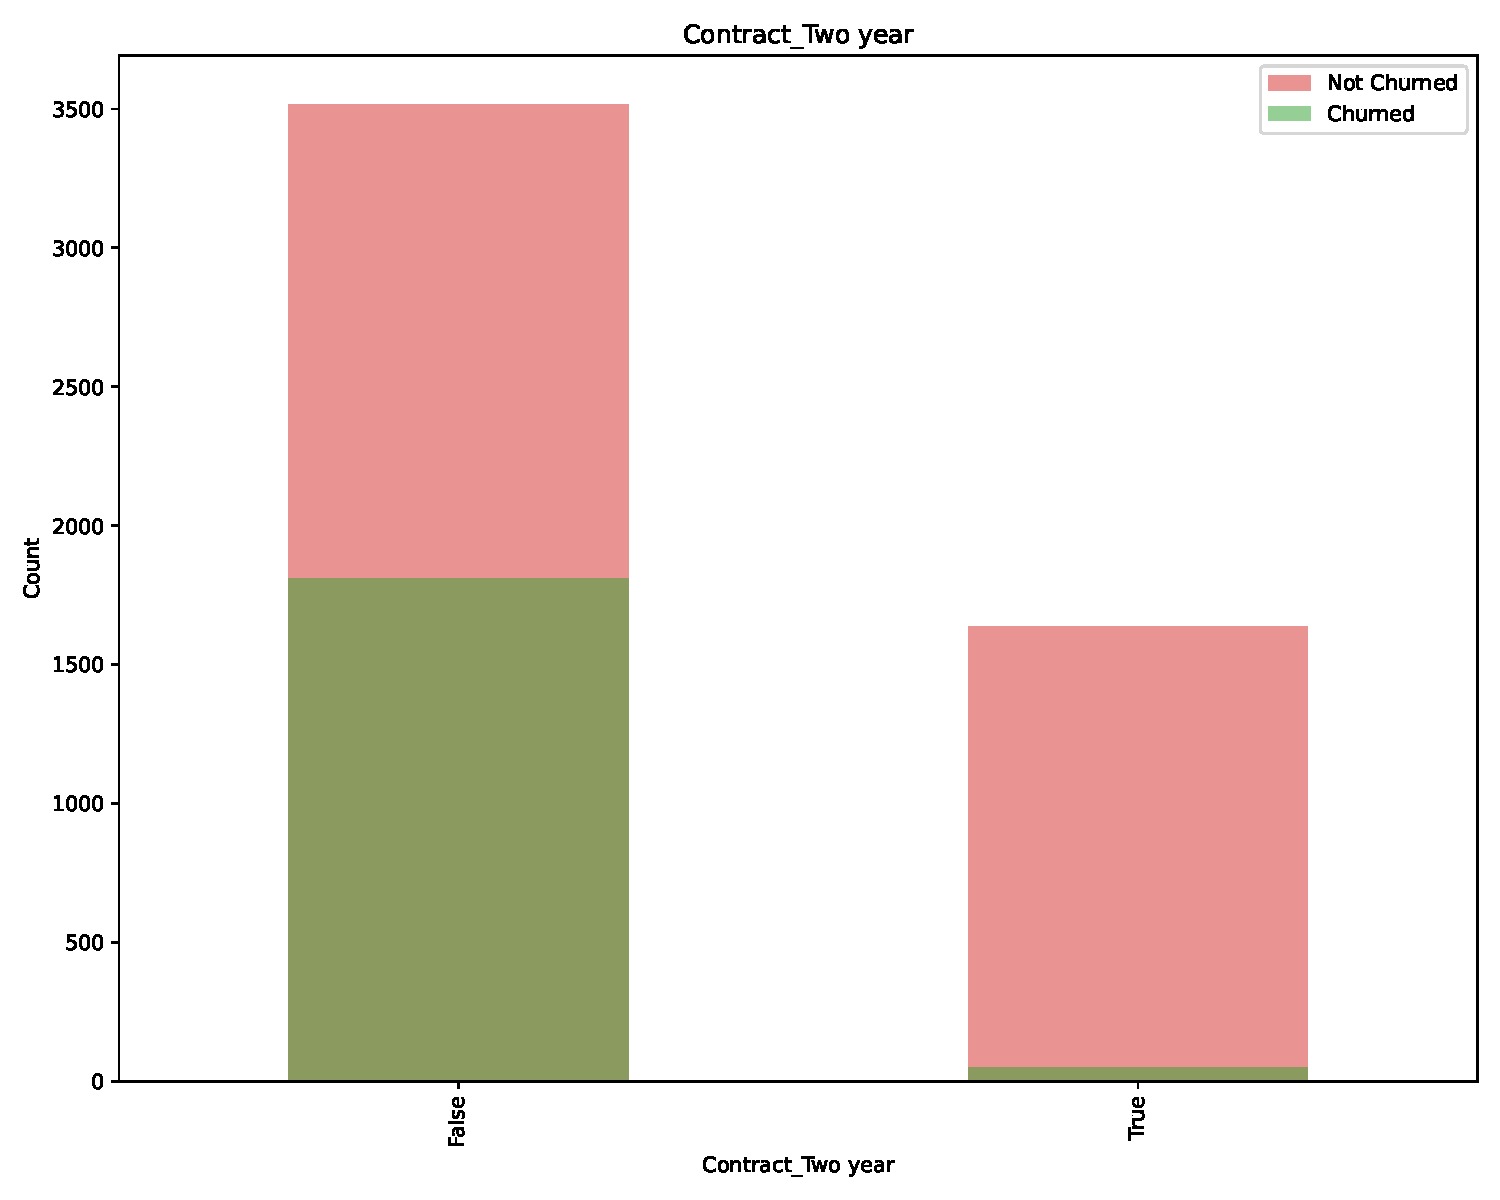
\includegraphics[width=\linewidth]{figures/understanding/Contract_Two year.pdf} 
    \caption{Contract [Two-Year]}
\end{subfigure}
\begin{subfigure}{0.14\linewidth}
    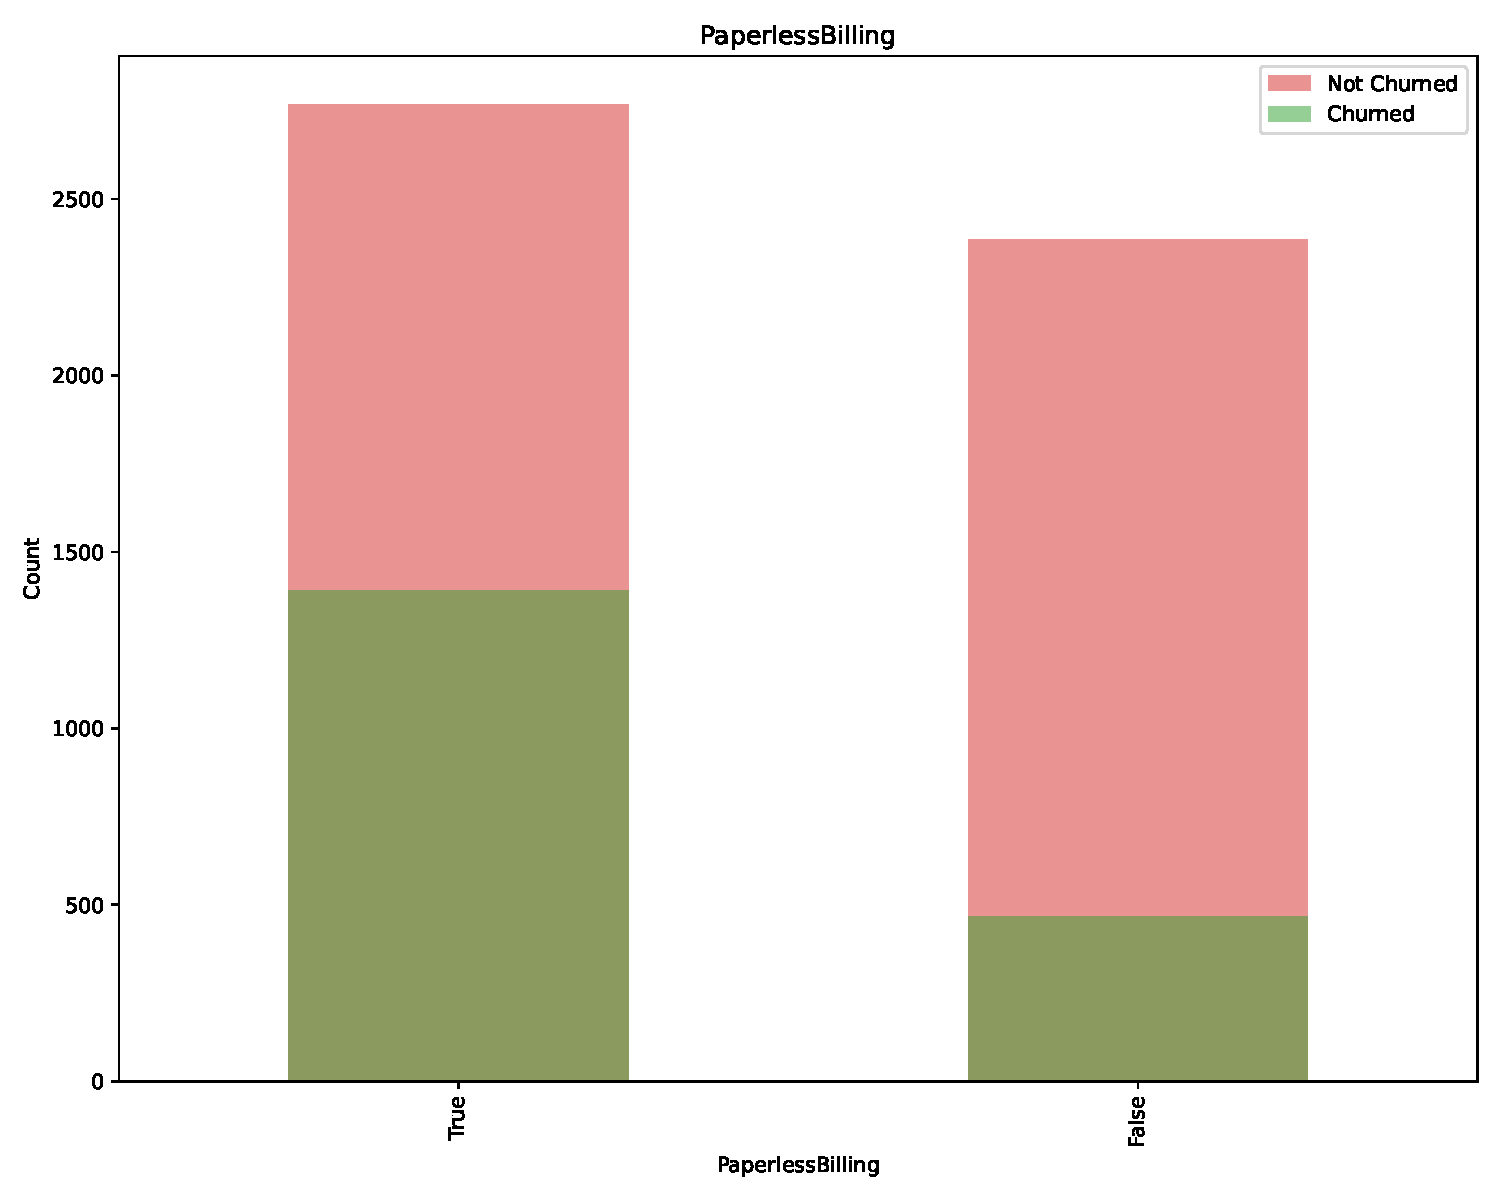
\includegraphics[width=\linewidth]{figures/understanding/PaperlessBilling.pdf}
    \caption{PaperlessBilling}
\end{subfigure}
\begin{subfigure}{0.14\linewidth}
    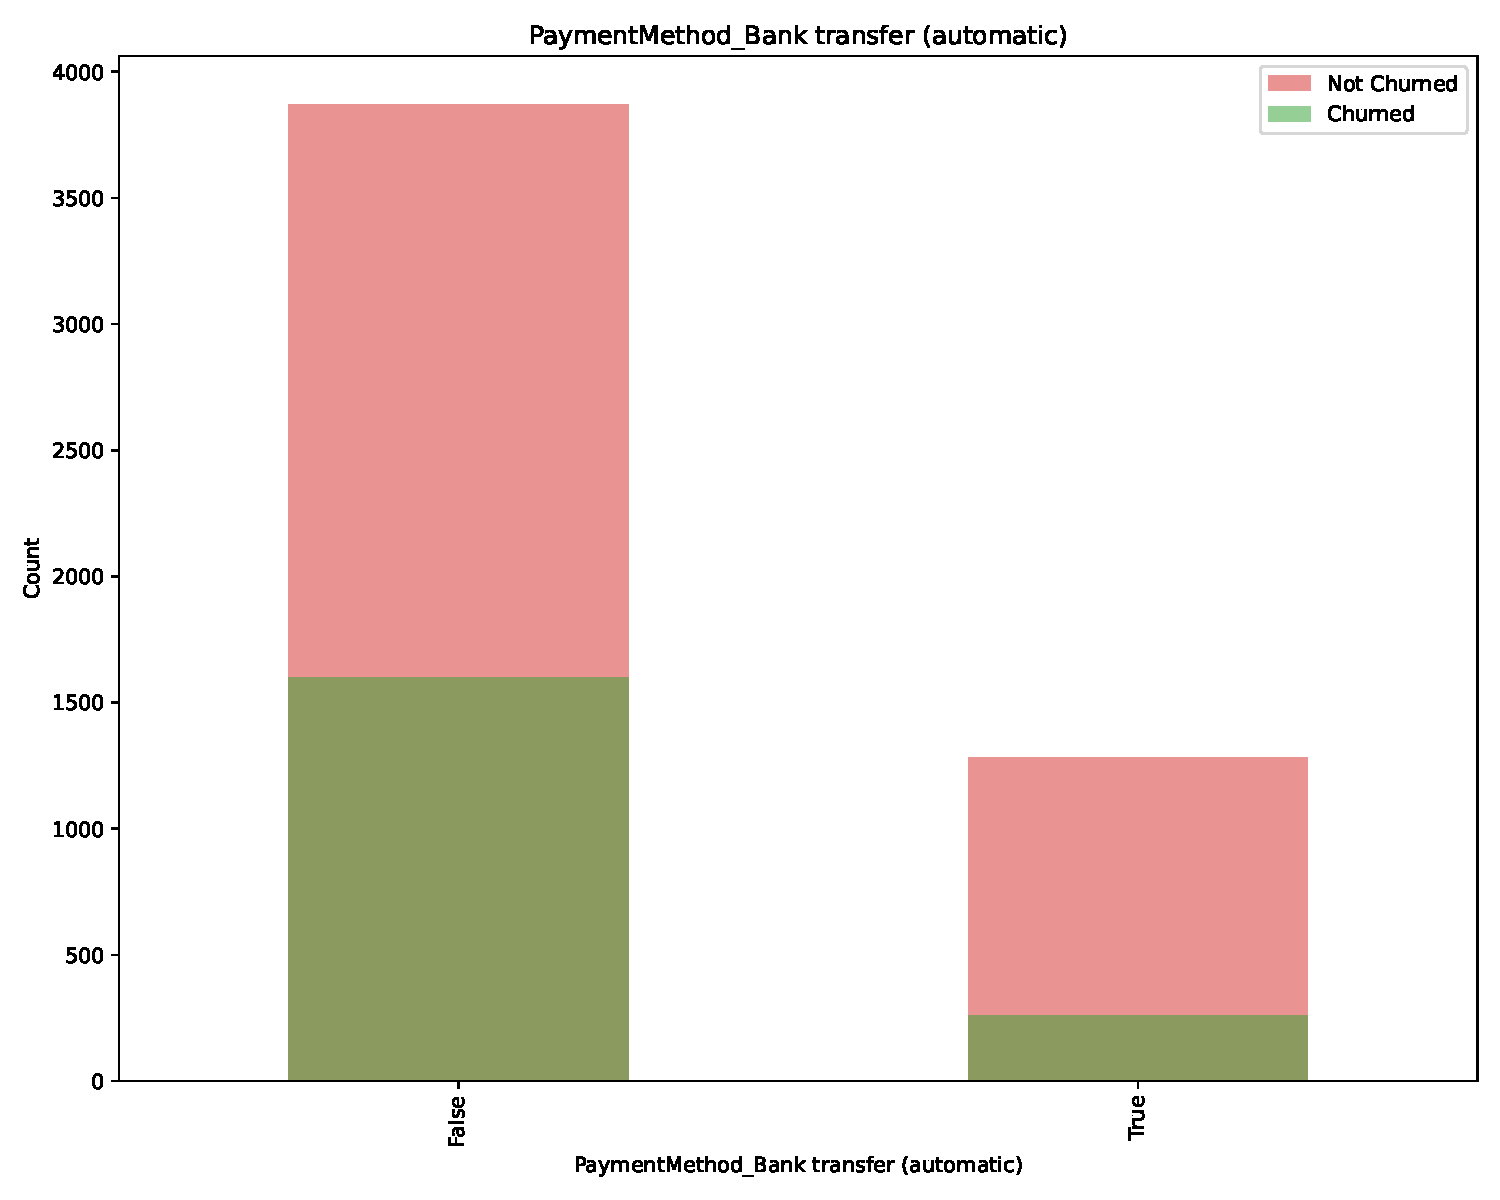
\includegraphics[width=\linewidth]{figures/understanding/PaymentMethod_Bank transfer (automatic).pdf}
    \caption{PaymentMethod [Bank Transfer]}
\end{subfigure}
\begin{subfigure}{0.14\linewidth}
    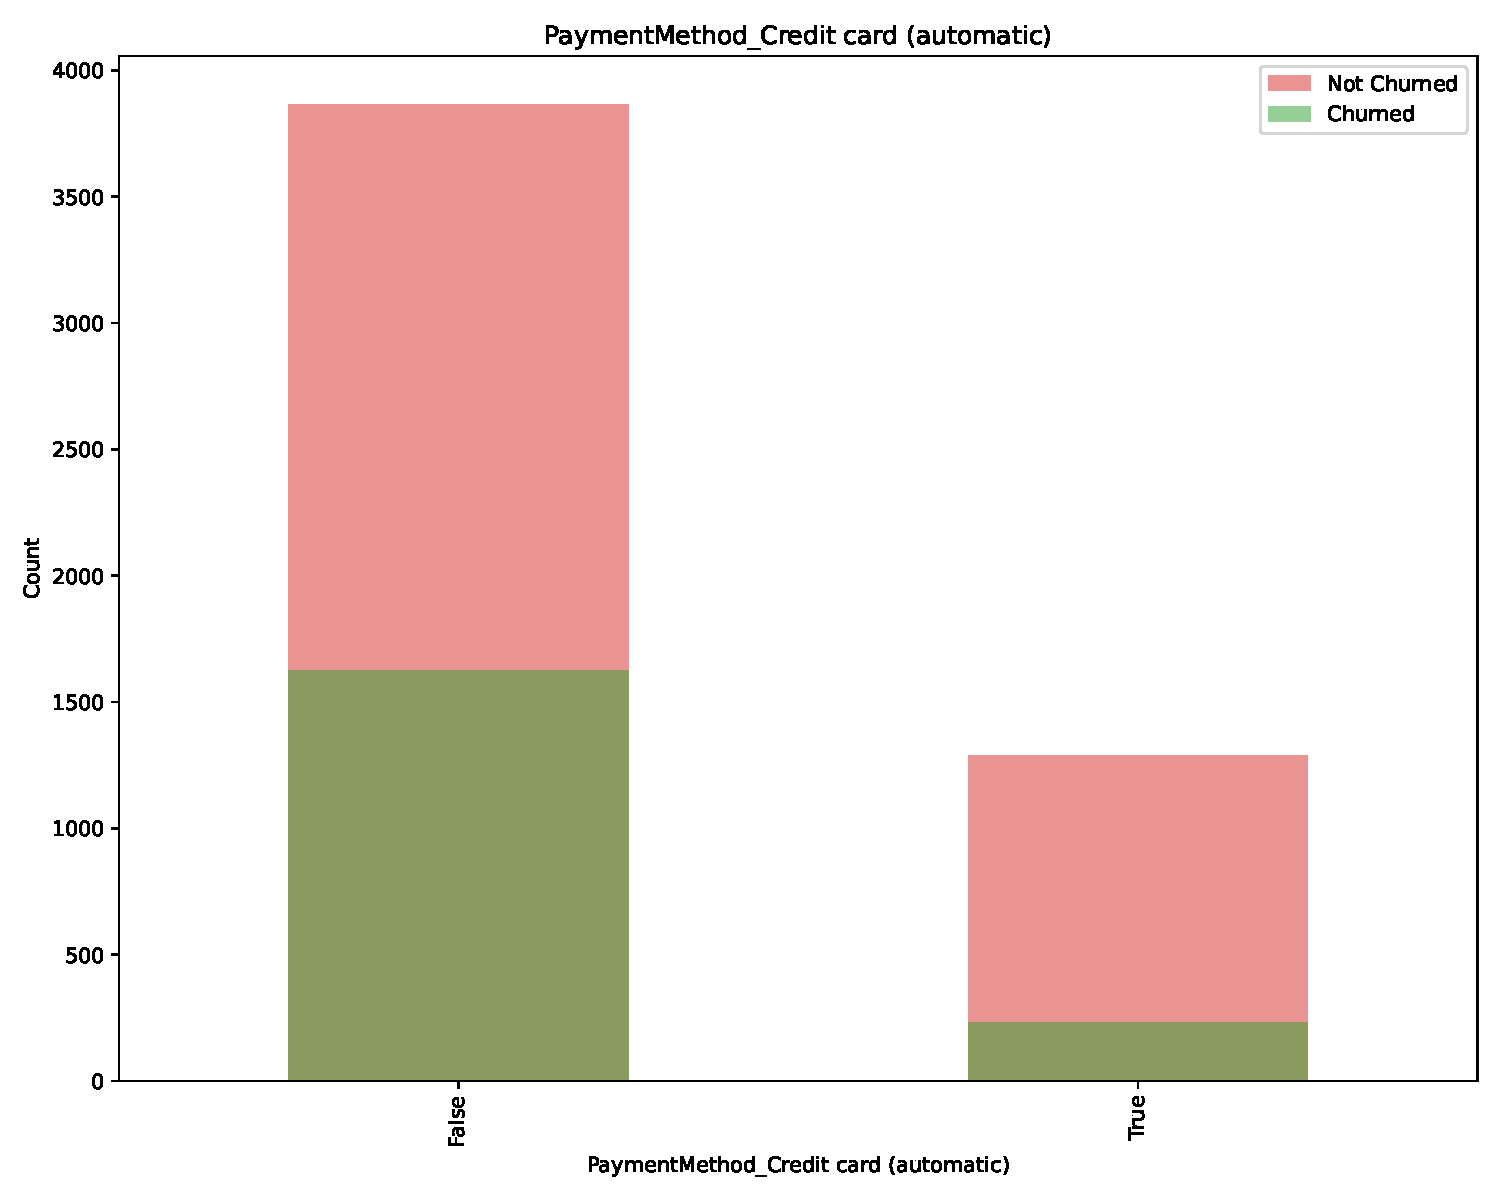
\includegraphics[width=\linewidth]{figures/understanding/PaymentMethod_Credit card (automatic).pdf}
    \caption{PaymentMethod [Credit Card]}
\end{subfigure}
\begin{subfigure}{0.14\linewidth}
    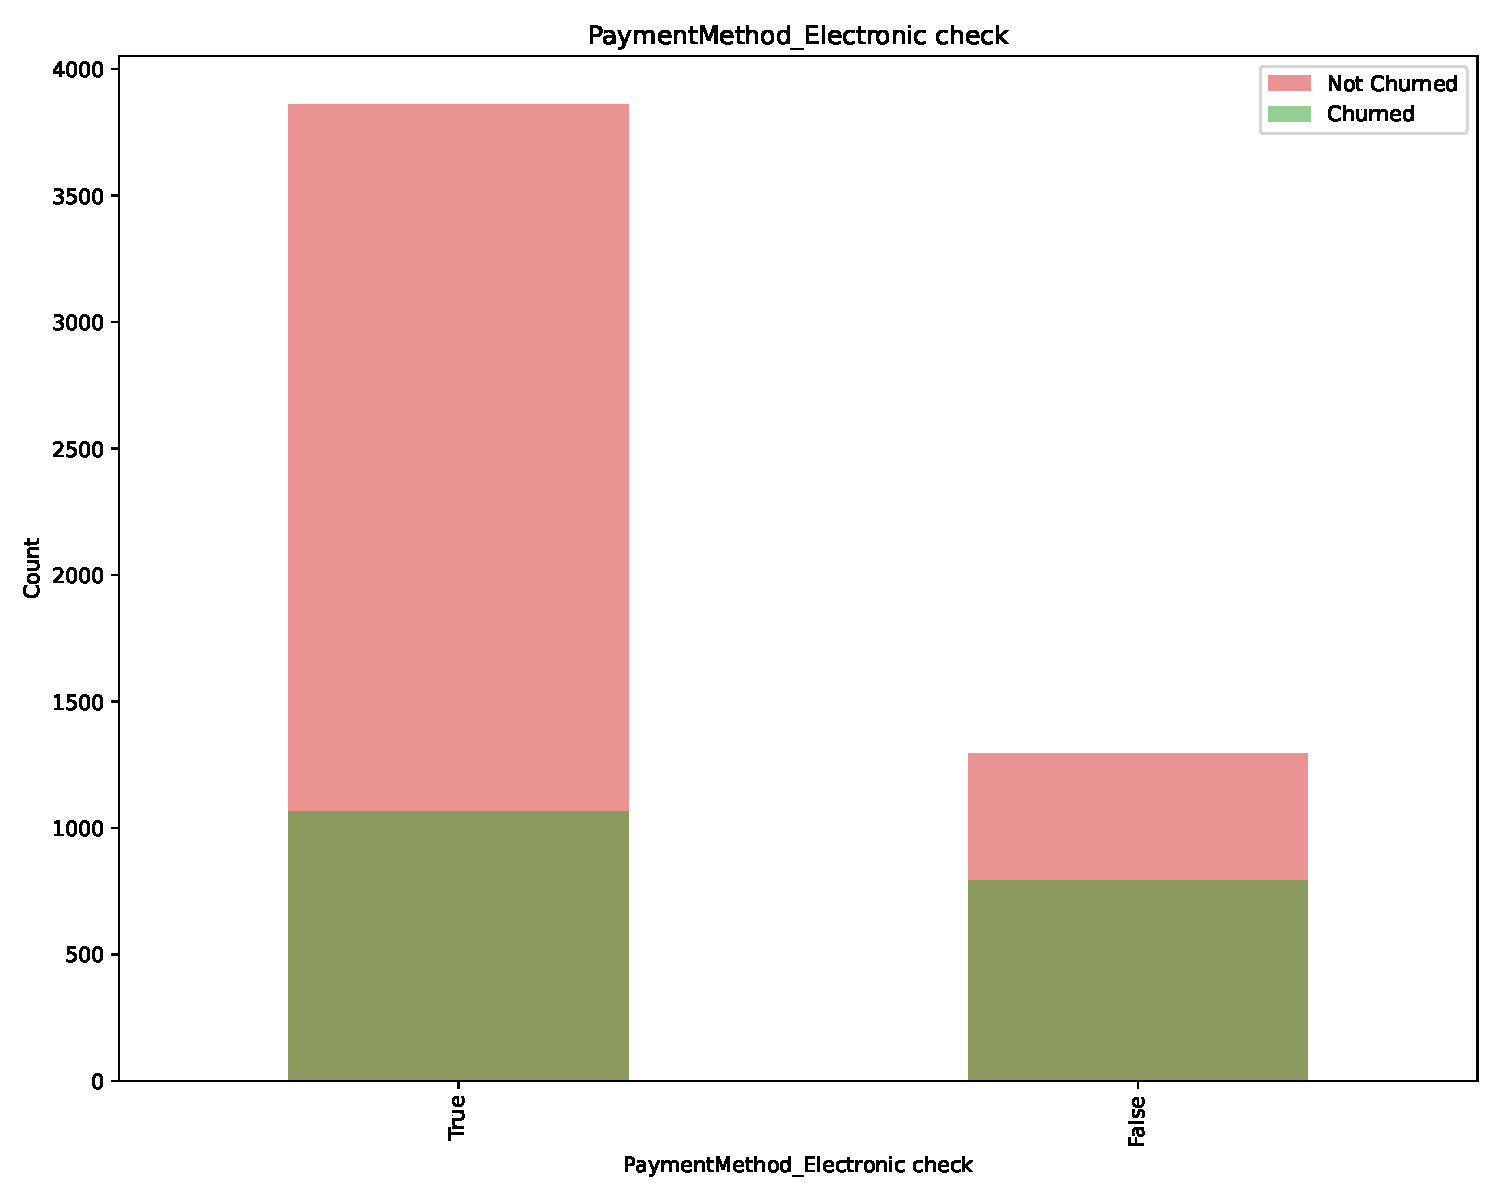
\includegraphics[width=\linewidth]{figures/understanding/PaymentMethod_Electronic check.pdf}
    \caption{PaymentMethod [E-Check]}
\end{subfigure}
\begin{subfigure}{0.14\linewidth}
    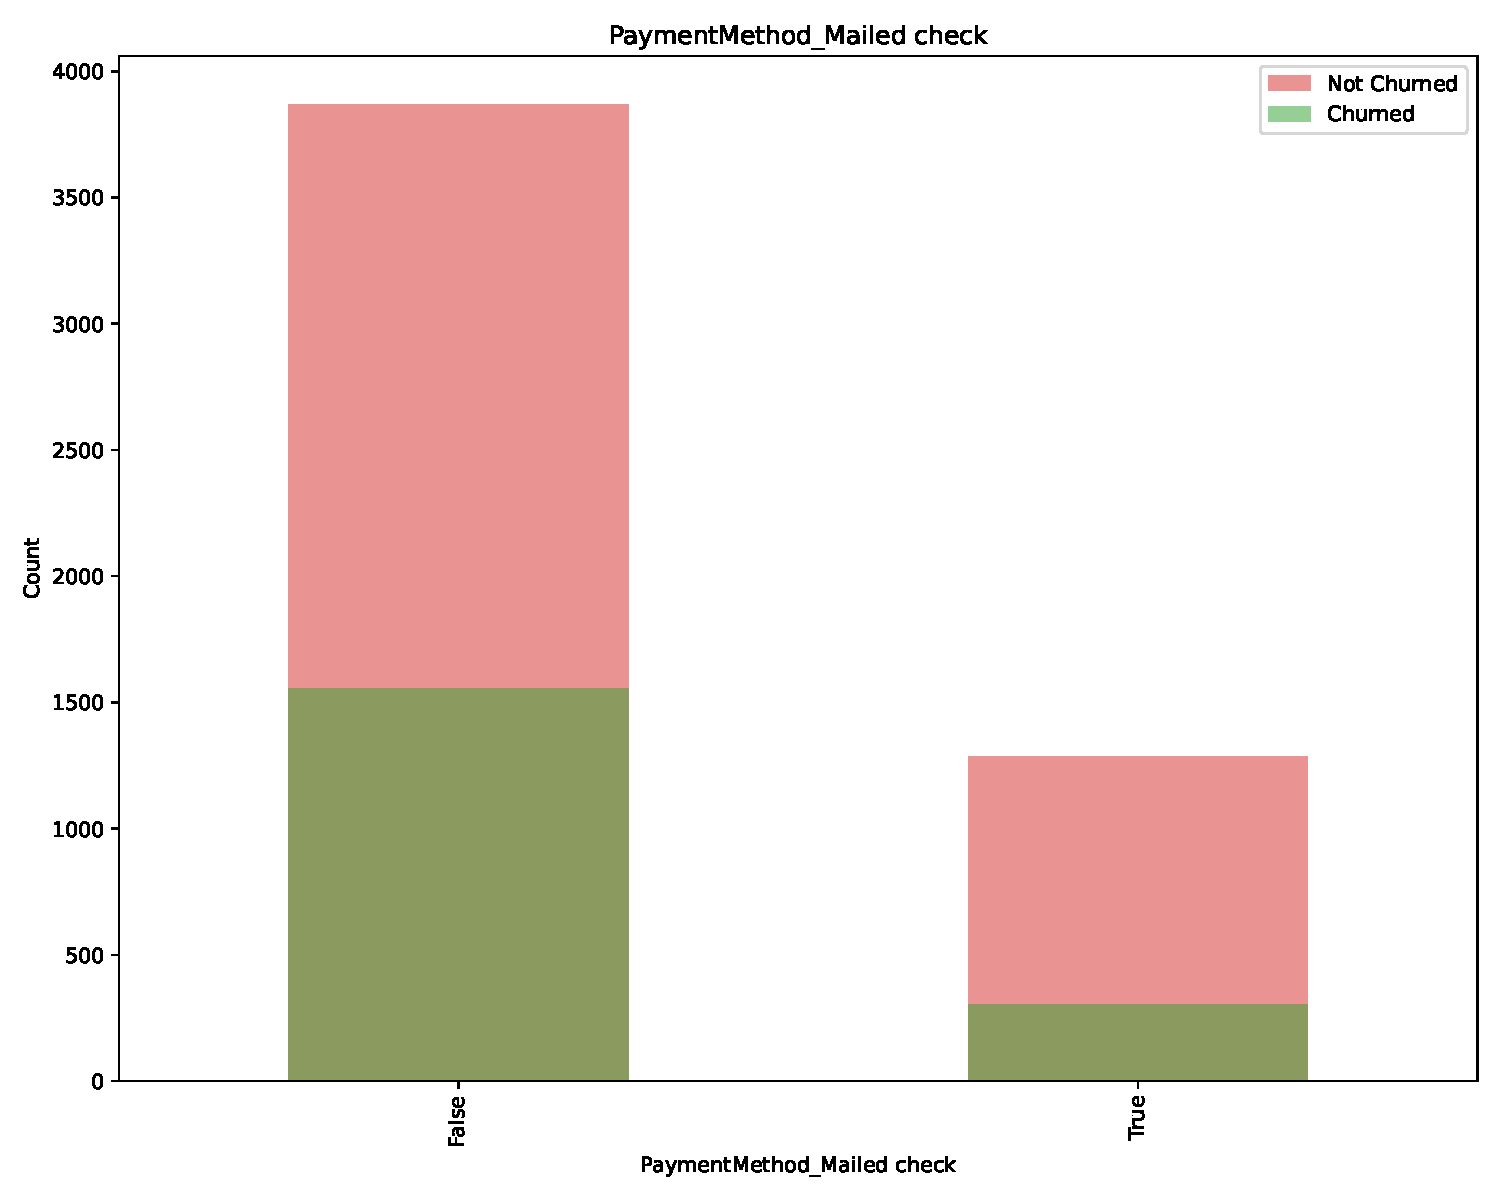
\includegraphics[width=\linewidth]{figures/understanding/PaymentMethod_Mailed check.pdf}
    \caption{PaymentMethod [Mailed check]}
\end{subfigure}
\begin{subfigure}{0.14\linewidth}
    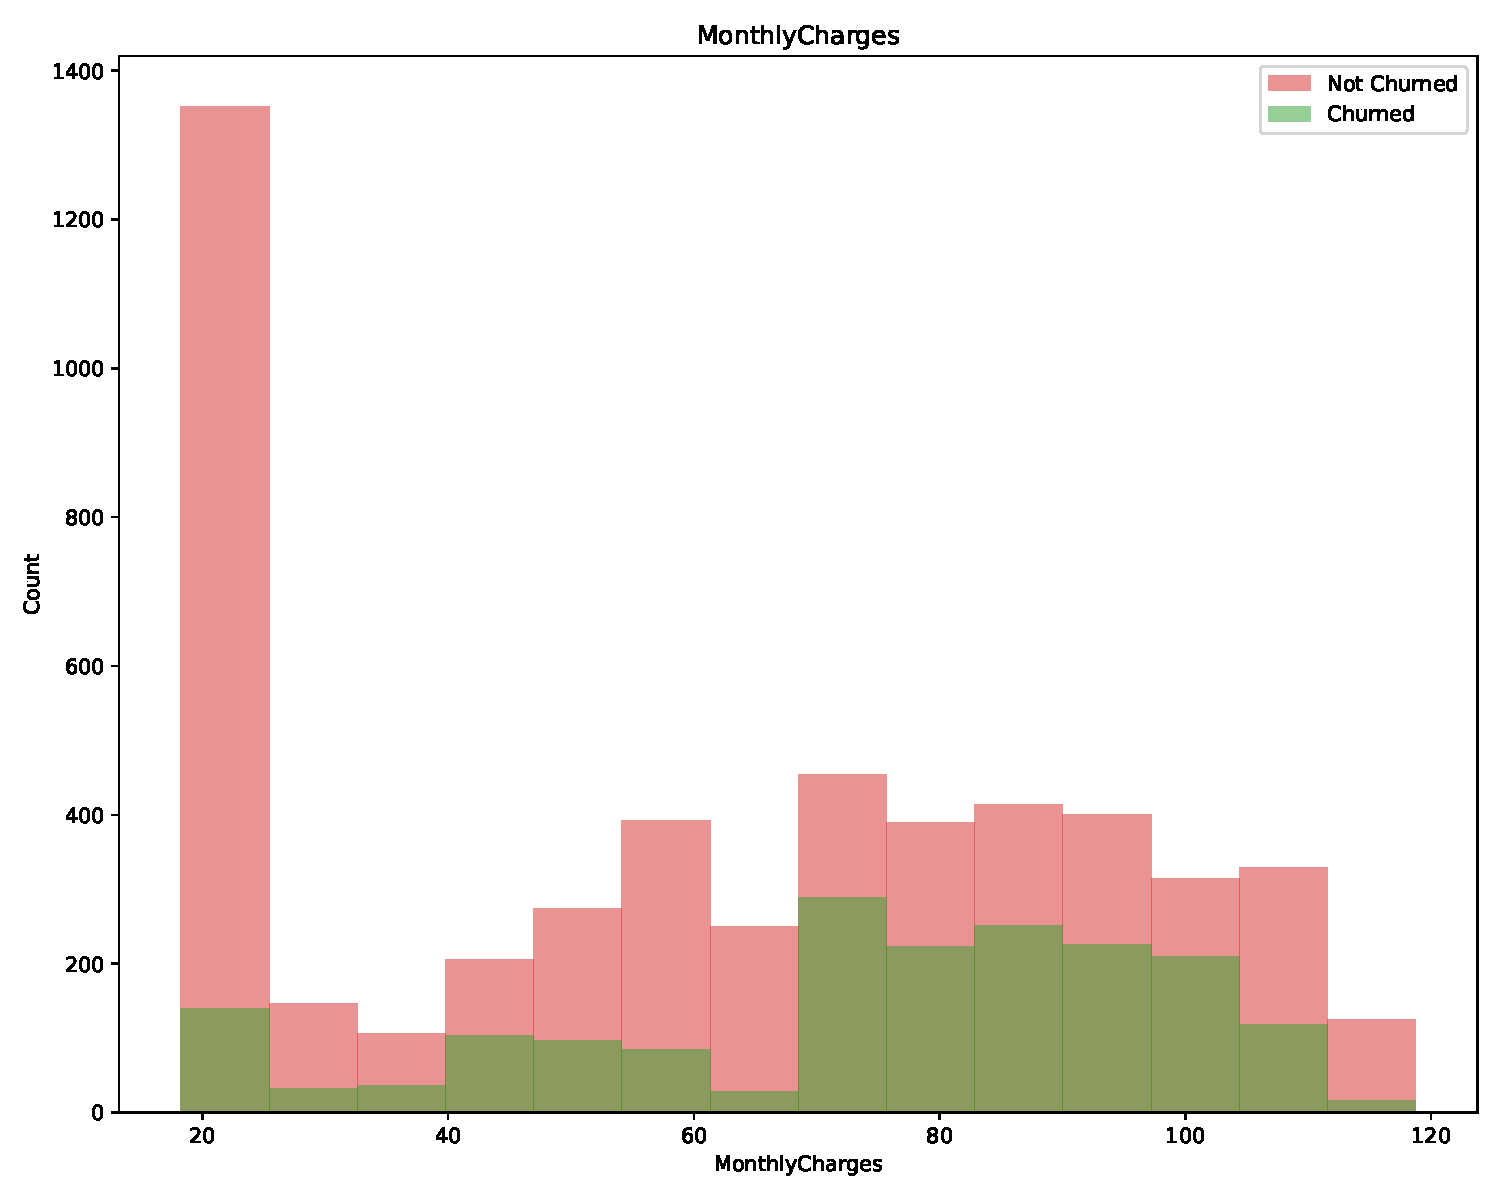
\includegraphics[width=\linewidth]{figures/understanding/MonthlyCharges.pdf}
    \caption{MonthlyCharges}
\end{subfigure}
\begin{subfigure}{0.14\linewidth}
    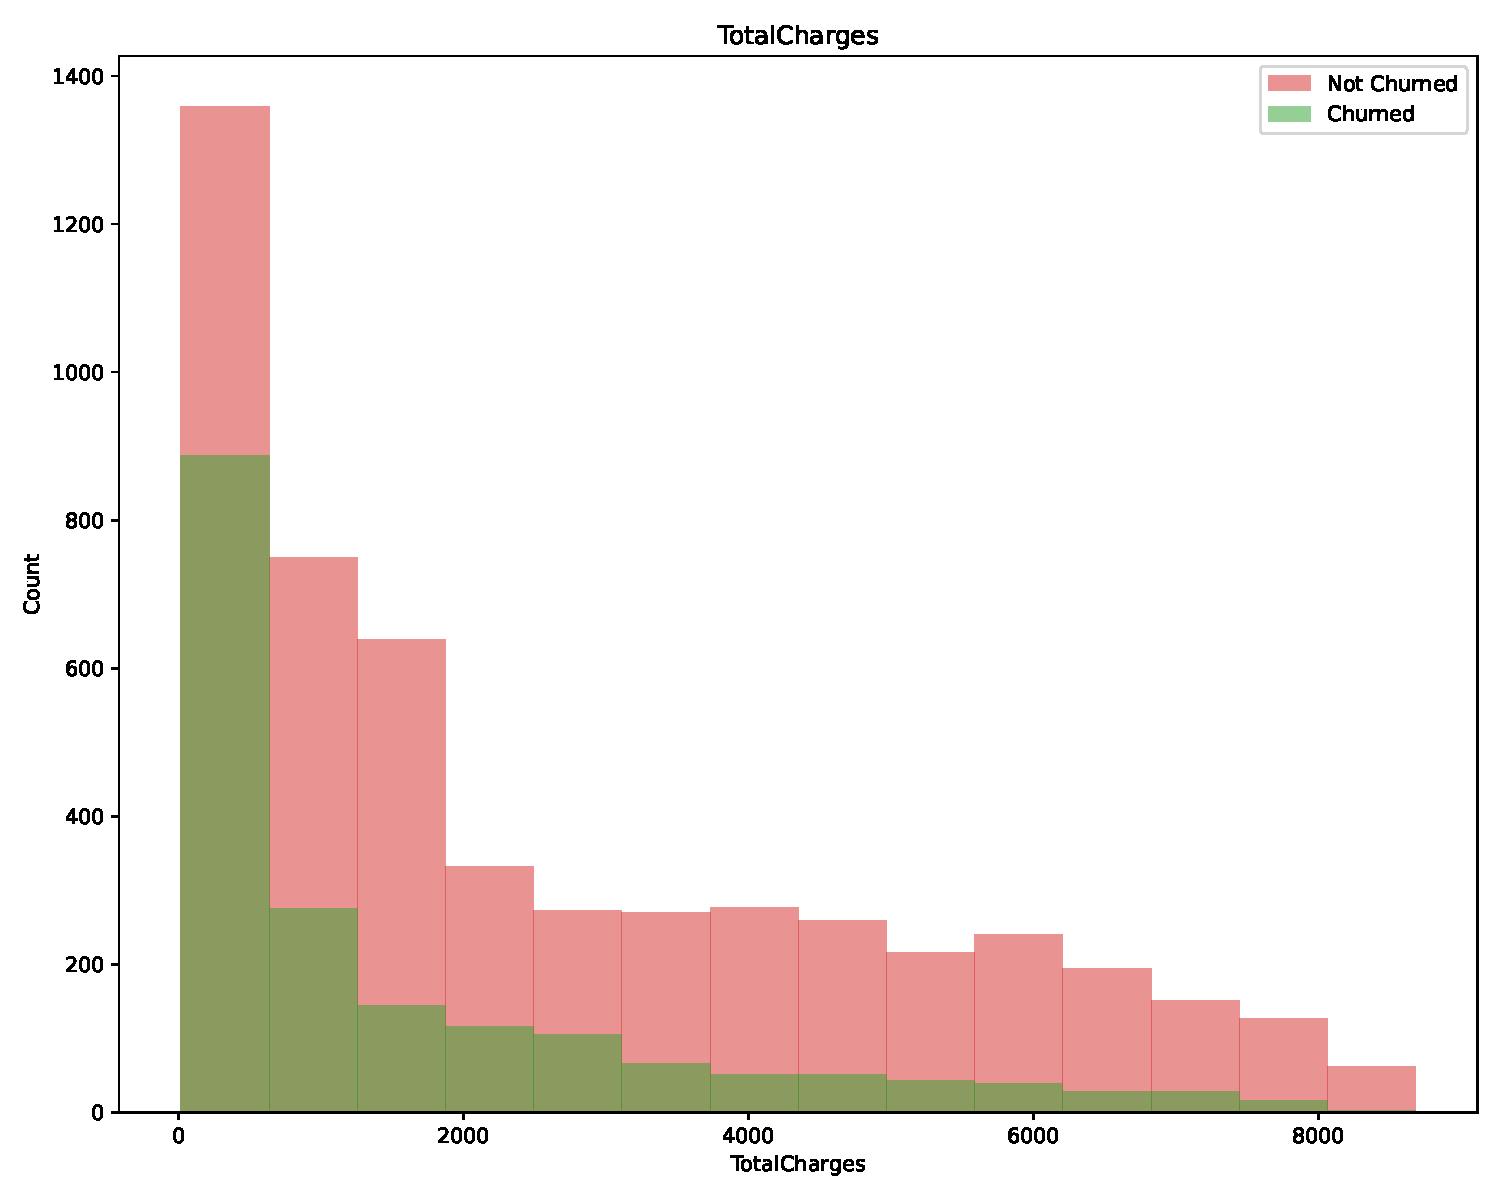
\includegraphics[width=\linewidth]{figures/understanding/TotalCharges.pdf}
    \caption{TotalCharges}
\end{subfigure}
\begin{subfigure}{0.14\linewidth}
    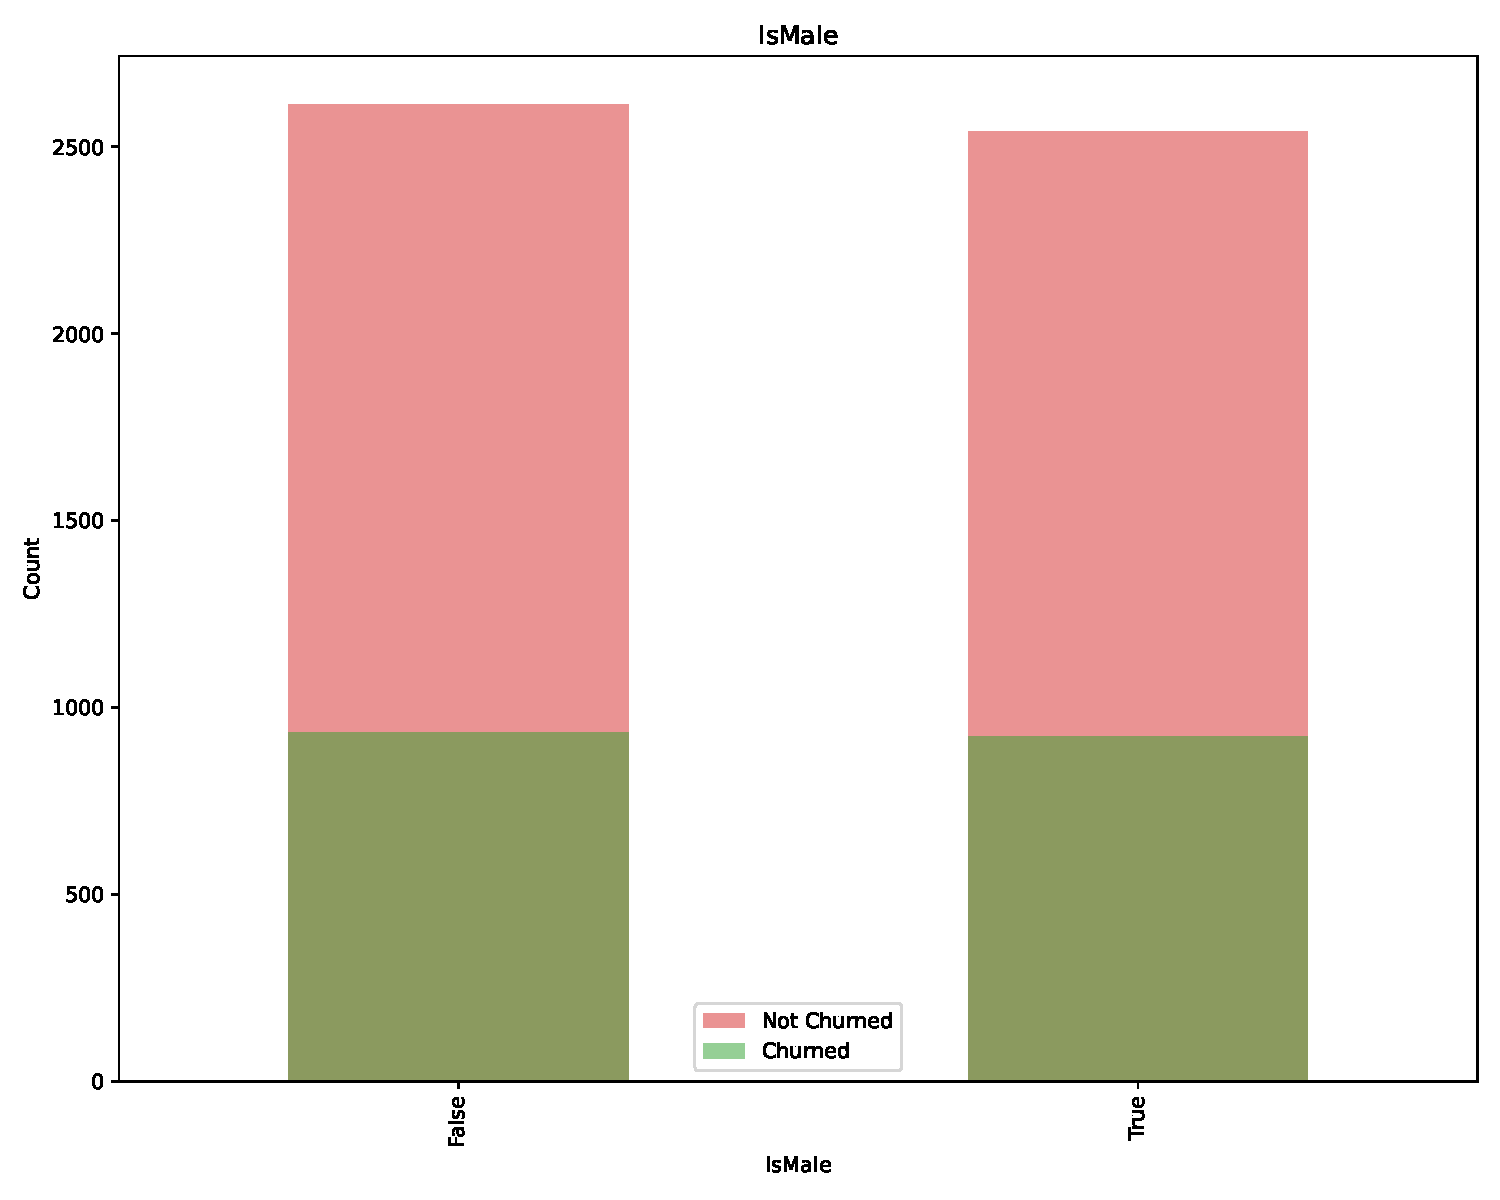
\includegraphics[width=\linewidth]{figures/understanding/IsMale.pdf}
    \caption{IsMale}
\end{subfigure}

\caption{Distributions of the dataset features after preprocessing.}
\label{fig:all_feature_histograms}
\end{figure}
\end{landscape}

\begin{figure}
\centering
\begin{subfigure}{\linewidth}
    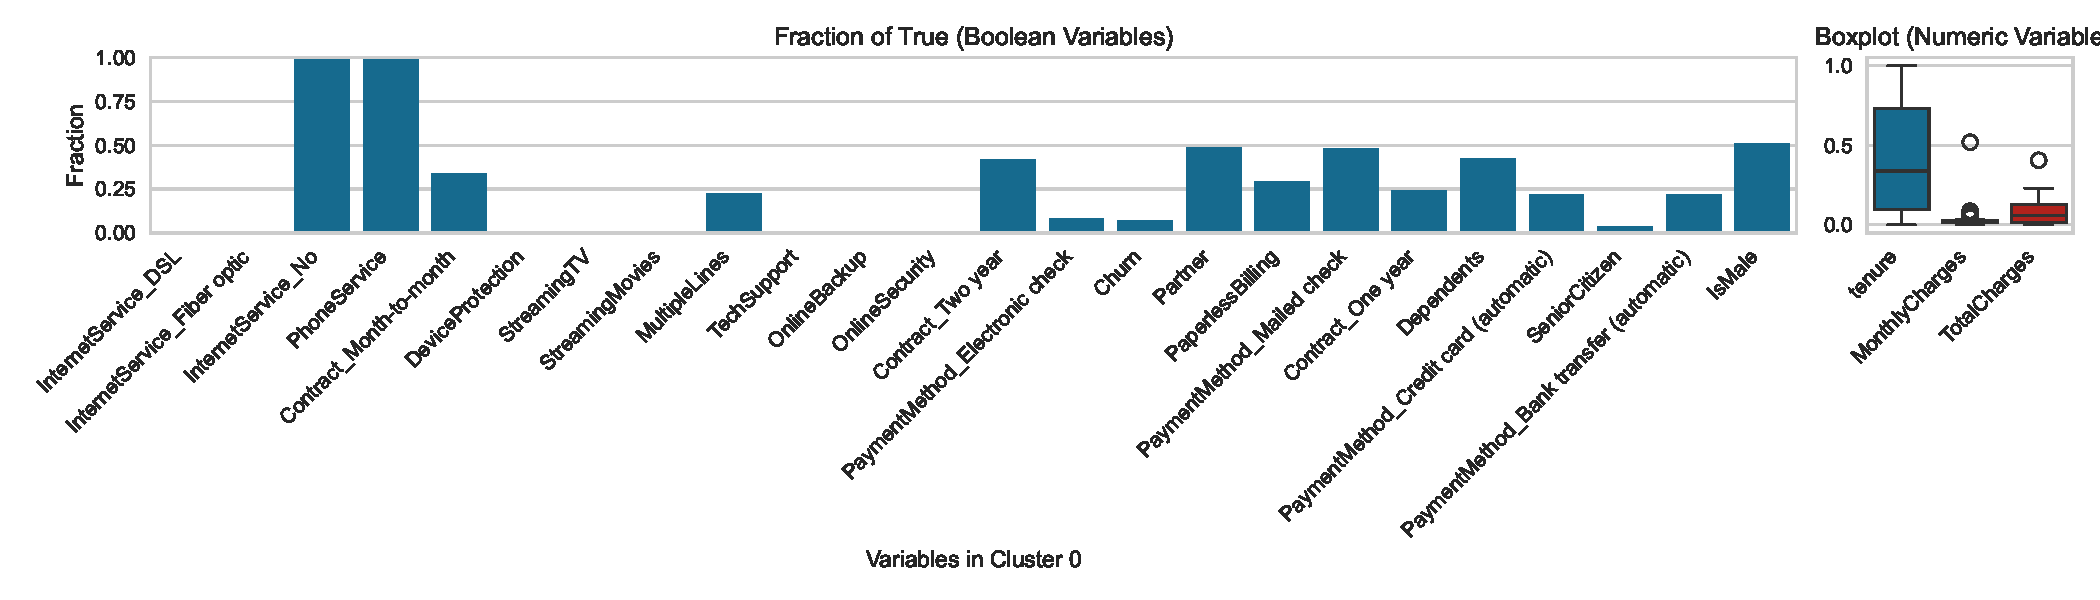
\includegraphics[width=\linewidth]{figures/clustering/cluster_0_clusters.pdf}
\caption{Cluster 0}
\label{fig:cluster_0}
\end{subfigure}
\begin{subfigure}{\linewidth}
    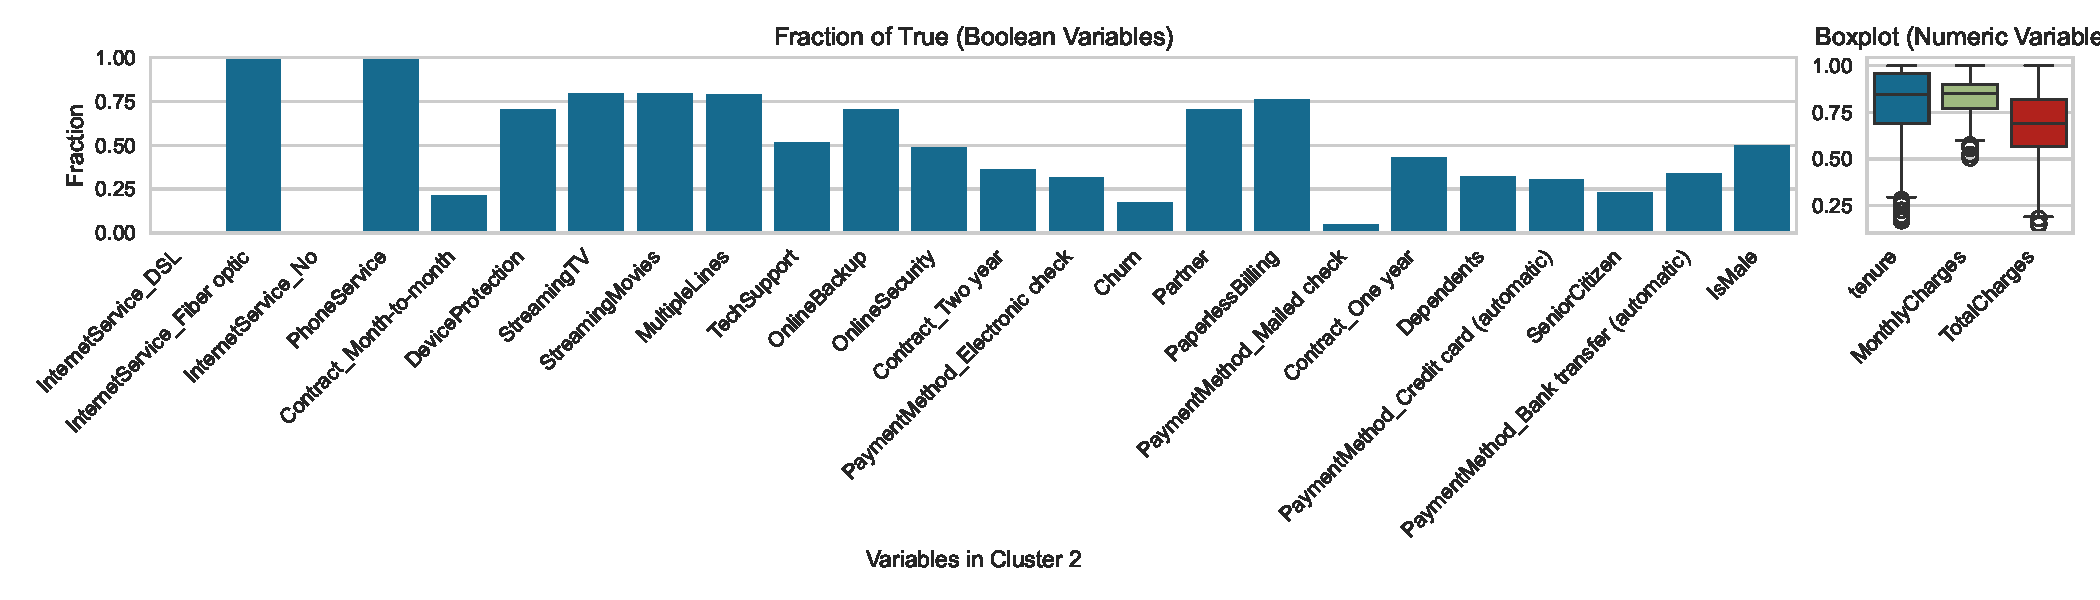
\includegraphics[width=\linewidth]{figures/clustering/cluster_2_clusters.pdf}
\caption{Cluster 2}
\label{fig:cluster_2}
\end{subfigure}
\begin{subfigure}{\linewidth}
    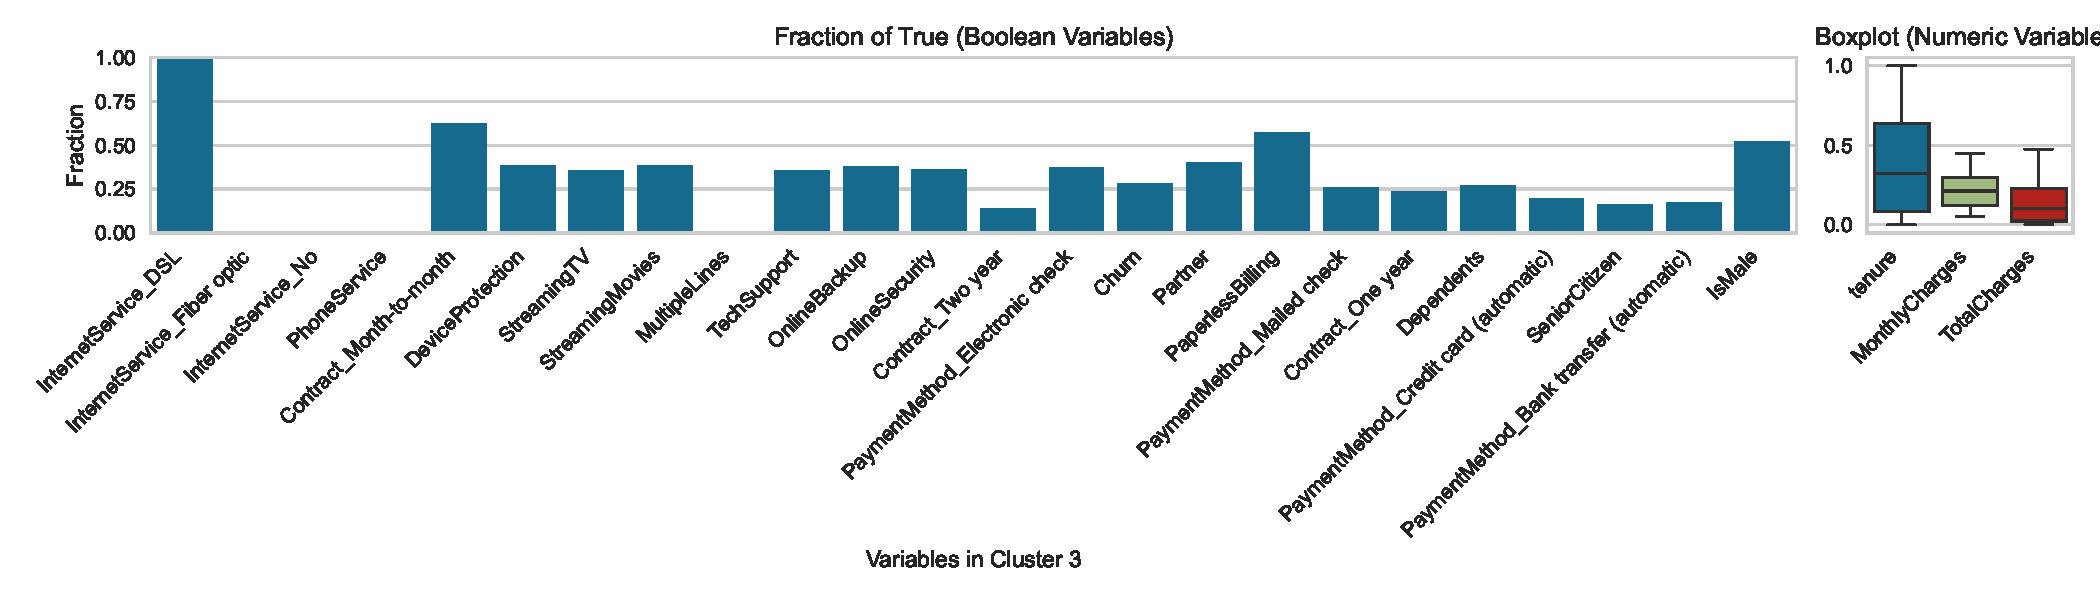
\includegraphics[width=\linewidth]{figures/clustering/cluster_3_clusters.pdf}
\caption{Cluster 3}
\label{fig:cluster_3}
\end{subfigure}
\begin{subfigure}{\linewidth}
    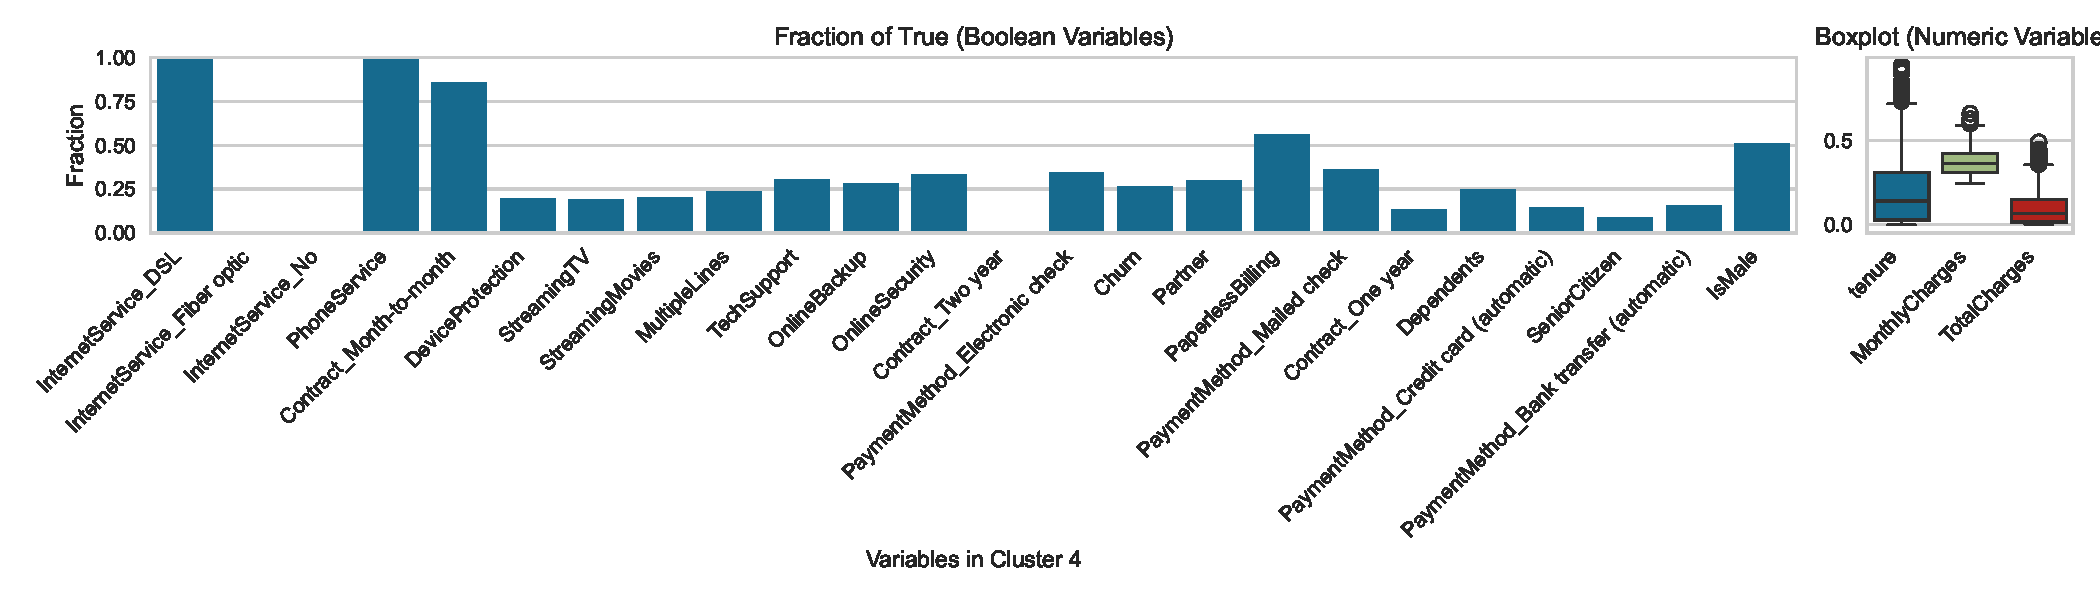
\includegraphics[width=\linewidth]{figures/clustering/cluster_4_clusters.pdf}
\caption{Cluster 4}
\label{fig:cluster_4}
\end{subfigure}
\caption{Distribution of features in the clusters (not shown in main). For the boolean features only the percentage is reported in the form of a bar plot, while the distribution of the normalized numerical features is represented with boxplots}
\end{figure}

\begin{figure}
\centering
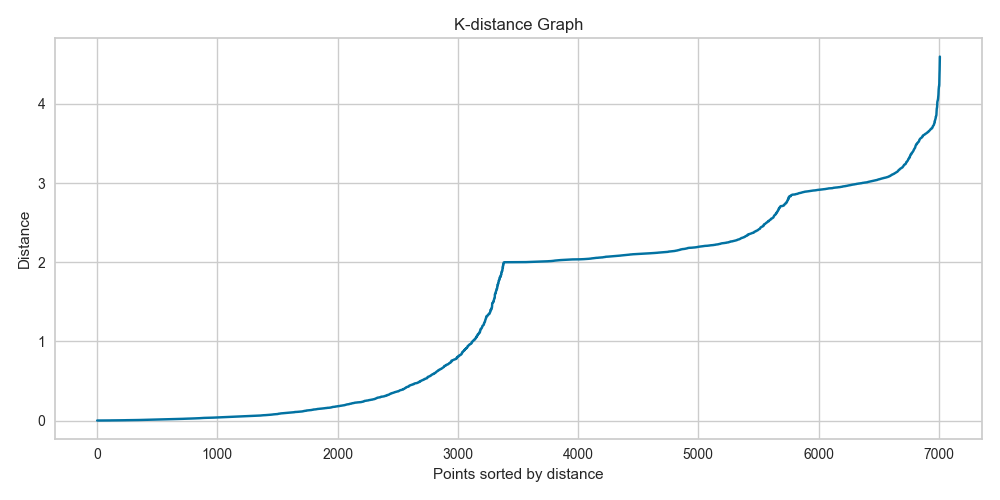
\includegraphics[width=\linewidth]{figures/clustering/dbscan_k_distance.png}
\caption{kNN in PCA space with k=5. Analysis performed for choice of parameter $\epsilon$ in DBSCAN. }
\label{fig:kNN_PCA}
\end{figure}

\begin{figure}
\centering
\begin{subfigure}{0.49\linewidth}
    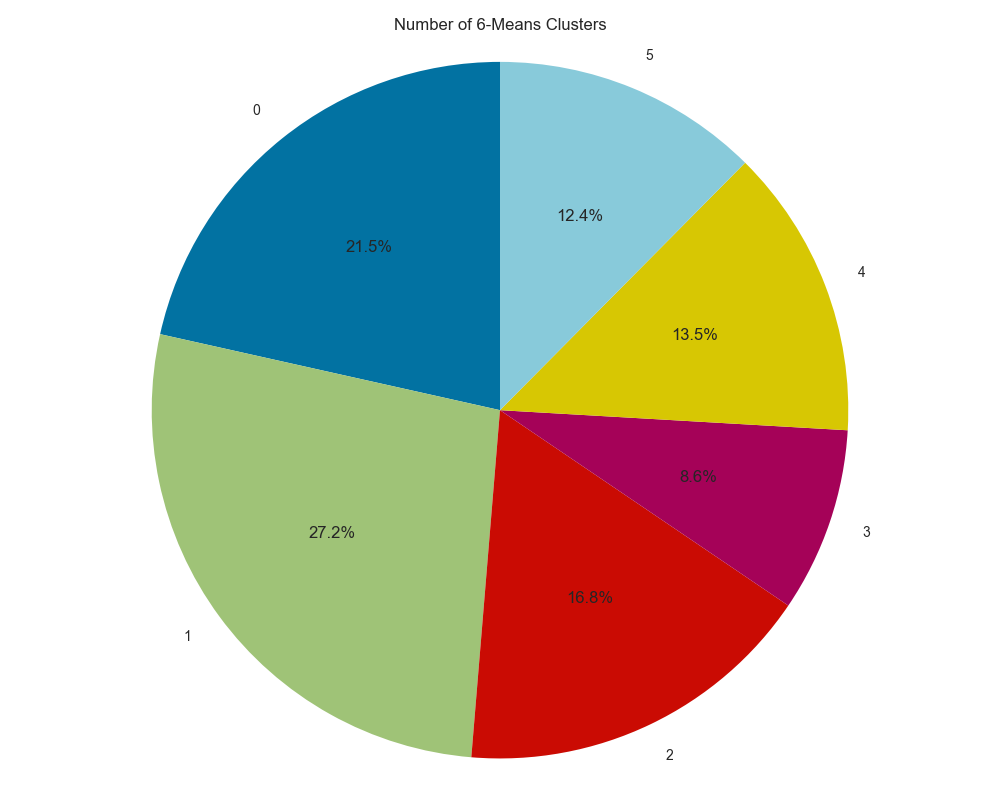
\includegraphics[width=\linewidth]{figures/clustering/6-means_pie.png}
\caption{6-Means}
\label{fig:pie_kmeans}
\end{subfigure}
\begin{subfigure}{0.5\linewidth}
    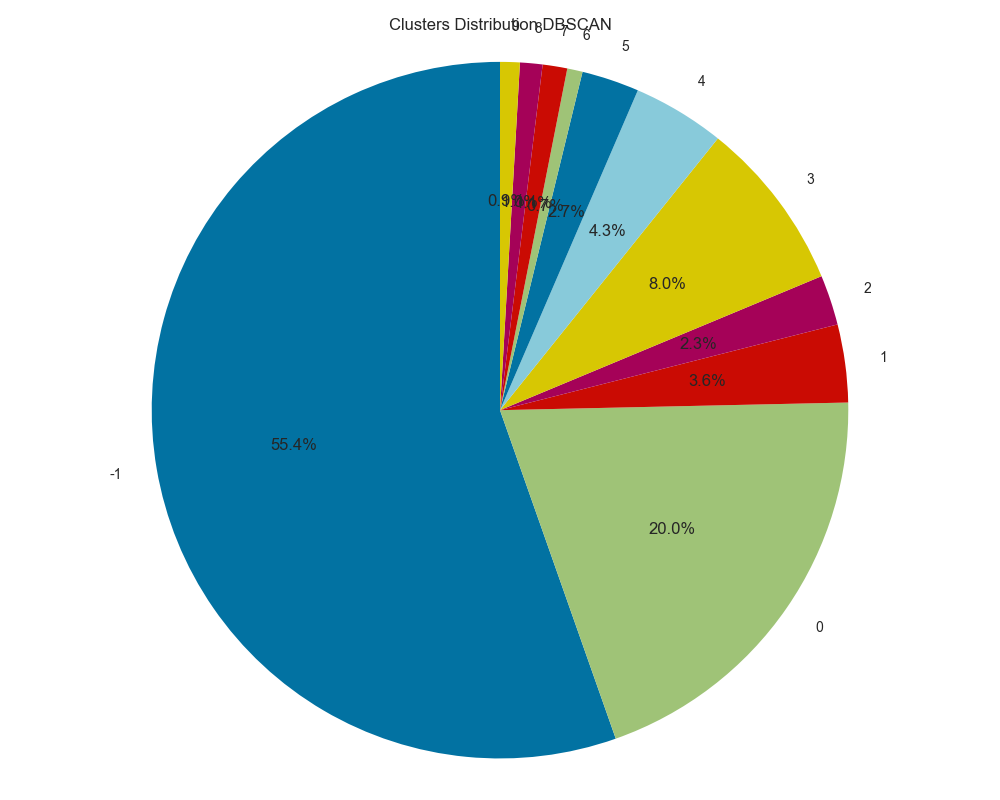
\includegraphics[width=\linewidth]{figures/clustering/dbscan_pie.png}
\caption{DBSCAN}
\label{fig:pie_dbscan}
\end{subfigure}
\caption{Number of points in each cluster for both k-Means (with k=6) and DBSCAN. The majority points found by DBSCAN are classified as outliers (\texttt{cluster\_id}=-1)}
\end{figure}

\begin{figure}
    \centering
    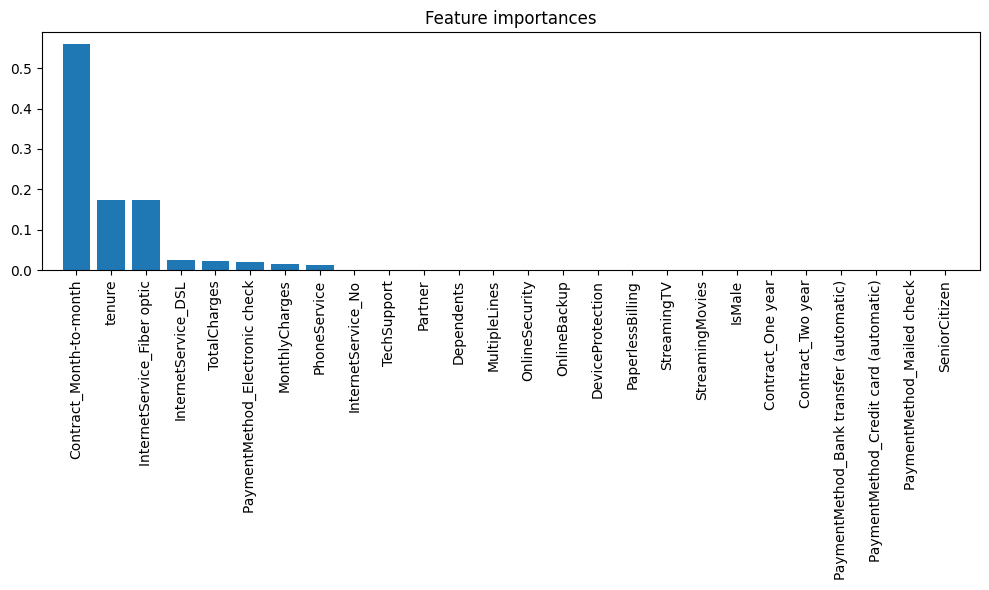
\includegraphics[width=\linewidth]{figures/classification/feature_importance_dt.png}
    \caption{Feature Importance from Decision Tree classifier}
    \label{fig:dt_ft}
\end{figure}

\begin{figure}
    \centering
    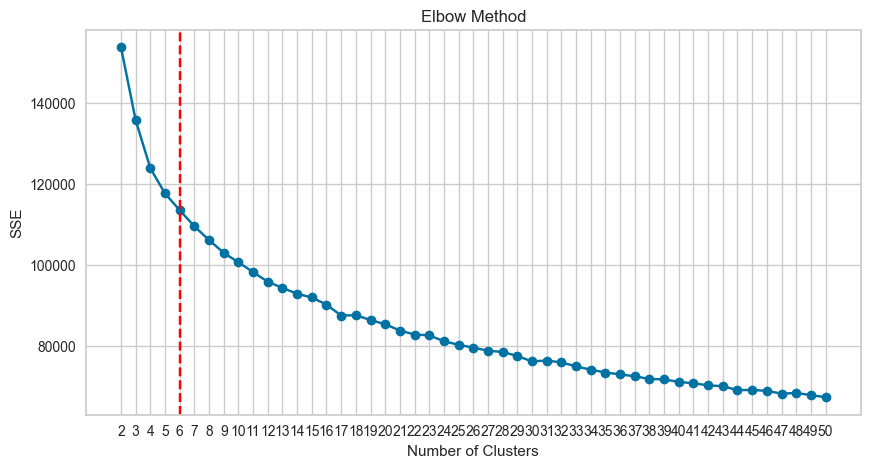
\includegraphics[width=\linewidth]{figures/clustering/elbow.png}
    \caption{Elbow Method for determining the best value of K for K-Means algorithm}
    \label{fig:km}
\end{figure}


\end{document}
